\documentclass[c]{beamer}

\usepackage{csquotes}
\usepackage{multirow}
\usepackage{pgfplots}
\usepackage{pgfplotstable}
\usepackage{subcaption}
\usepackage{transparent}
\usepackage{tikz}
\usepackage{xcolor}

\usepgfplotslibrary{fillbetween}
\usepgfplotslibrary{groupplots}
\usepgfplotslibrary{statistics}

\usetikzlibrary{arrows.meta}
\usetikzlibrary{calc}
\usetikzlibrary{shapes}

\usetheme{metropolis}
\author{Esten H{\o}yland Leonardsen}
\title{Detecting individual-level deviations in brain morphology with Layerwise Relevance Propagation}

\definecolor{cb-pink}{HTML}{eeafcf}
\definecolor{cb-orange}{HTML}{e59145}
\definecolor{cb-light-brown}{HTML}{baa066}
\definecolor{cb-blue}{HTML}{3594d6}
\definecolor{cb-green}{HTML}{4dac93}
\definecolor{cb-gray}{HTML}{3a5c7d}
\definecolor{cb-light-purple}{HTML}{b45899}
\definecolor{cb-red-purple}{HTML}{c71555}
\definecolor{cb-brown}{HTML}{840000}
\definecolor{cb-blue-purple}{HTML}{662fa2}

\colorlet{cases-default}{cb-red-purple}
\colorlet{controls-default}{cb-blue}

\newcommand{\N}{5}

\begin{document}
	\begin{frame} % Title
		\maketitle
	\end{frame}
	
	\begin{frame}{Explainable AI: Motivation} % Blackbox
		\vfill
		\centering
		\begin{tikzpicture}
			\node[draw=black,fill=white,inner sep=0pt]{
				\includegraphics[width=8cm]{data/blackbox.jpg}
			};
		\end{tikzpicture}
		\vfill
	\end{frame}
	
	\begin{frame}{Explainable AI: Motivation} % Linear algebra
		\vfill
		\centering
		\begin{tikzpicture}
			\node[draw=black,fill=white,inner sep=1pt]{
				\includegraphics[width=6cm]{data/meme.jpg}
			};
		\end{tikzpicture}
		\vfill
	\end{frame}
	
	\begin{frame}{Explainable AI: Motivation} % Model complexity
		\vfill
		\centering
		\includegraphics[width=4cm]{data/oom.png}
		\vfill
	\end{frame}
	
	{
    	\setbeamertemplate{footline}{\hspace{0.33cm}\hfill \textcolor{gray}{\tiny{Kundu, S. AI in medicine must be explainable. Nat Med 27, 1328 (2021)}} \hfill \scriptsize{5} \hspace{0.26cm}\vspace{0.4cm}}
		\begin{frame}{Explainable AI: Motivation} % Quote
			\centering
			\vfill
			\textit{\enquote{Relying on devices whose logic is opaque violates principles of medical ethics.}}
			\vfill
		\end{frame}
	}
	
	{
    	\setbeamertemplate{footline}{\hspace{0.33cm}\hfill \textcolor{gray}{\tiny{Samek, et al., Explainable AI: interpreting, explaining and visualizing deep learning. Springer Nature, 2019}} \hfill \scriptsize{6} \hspace{0.26cm}\vspace{0.4cm}}
		\begin{frame}{Explainable AI: Overview}	% Explainable AI
			\vfill
			\centering
			\begin{tikzpicture}
				\node[draw=black,fill=white,inner sep=1pt]{
					\includegraphics[width=3cm]{data/book.jpeg}
				};
			\end{tikzpicture}
			\vfill
		\end{frame}
	}
	
	\begin{frame}{Explainable AI: Overview} % Overview
		\centering
		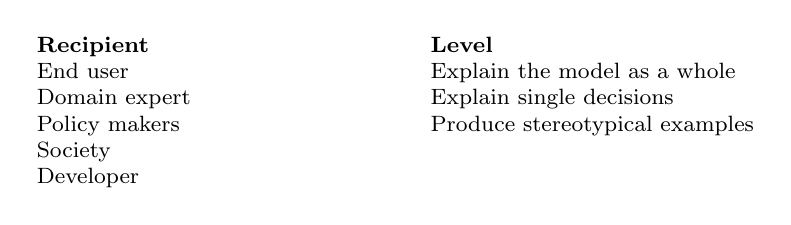
\begin{tikzpicture}
			\node[font=\footnotesize, align=left, anchor=north west] at (0,0) {
				\textbf{Recipient}\\
				End user\\
				Domain expert\\
				Policy makers\\
				Society\\
				Developer
			};
			
			\node[font=\footnotesize, align=left, anchor=north west] at (5,0) {
				\textbf{Level}\\
				Explain the model as a whole\\
				Explain single decisions\\
				Produce stereotypical examples
			};
		\end{tikzpicture}
	\end{frame}
	
	\begin{frame}{Explainable AI: Overview} % Overview
		\centering
		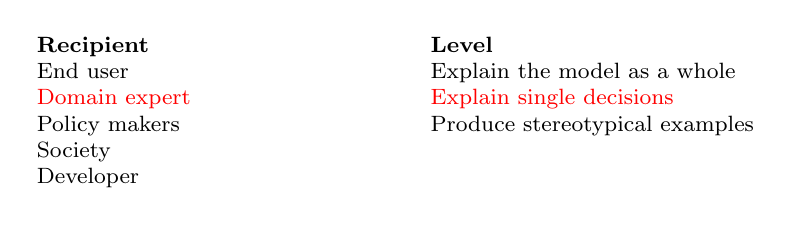
\begin{tikzpicture}
			\node[font=\footnotesize, align=left, anchor=north west] at (0,0) {
				\textbf{Recipient}\\
				End user\\
				\textcolor{red}{Domain expert}\\
				Policy makers\\
				Society\\
				Developer
			};
			
			\node[font=\footnotesize, align=left, anchor=north west] at (5,0) {
				\textbf{Level}\\
				Explain the model as a whole\\
				\textcolor{red}{Explain single decisions}\\
				Produce stereotypical examples
			};
		\end{tikzpicture}
	\end{frame}
	
	\begin{frame}{Explainable AI: Overview} % Nature of explanations
		\centering
		\vfill
		\begin{tikzpicture}
			\node[] at (-5, -5) {};
			\node[] at (-2,1) {
				\includegraphics[width=3cm]{data/ladybug.png}
			};
			\node[minimum width=3cm,align=center, font=\small] at (2, 1) {
				This is a\\ ladybug because\\ of the red\\ back with\\ the black dots
			};
			\node[] at (5, 5) {};
		\end{tikzpicture}
		\vfill
	\end{frame}
	
	{
    	\setbeamertemplate{footline}{\hspace{0.33cm}\hfill \textcolor{gray}{\tiny{\href{https://lrpserver.hhi.fraunhofer.de/image-classification9}{https://lrpserver.hhi.fraunhofer.de/image-classification}}} \hfill \scriptsize{10} \hspace{0.24cm}\vspace{0.4cm}}
		\begin{frame}{Explainable AI: Overview} % Nature of explanations
			\centering
			\vfill
			\begin{tikzpicture}
				\node[] at (-5, -5) {};
				\node[] at (-2,1) {
					\includegraphics[width=3cm]{data/ladybug.png}
				};
				\node[] at (2, 1) {
					\includegraphics[width=3cm]{data/ladybug_explanation.png}
				};
				\node[] at (5, 5) {};
			\end{tikzpicture}
			
			\vfill
		\end{frame}
	}
	
	
	\begin{frame}{Explainable AI: Surrogate models}
		\begin{tikzpicture}
			\node[] at (-5,-5) {};
			\node[] at (5,5) {};
			\node[inner sep=0pt] (ladybug) at (-3, 3) {
				\includegraphics[width=1cm]{data/ladybug.png}
			};
			\node[minimum width=1cm, minimum height=1cm, fill=black, inner sep=0pt,label=\tiny{model}] (model) at (0, 3) {};
			\node[] (prediction) at (3, 3) {\footnotesize{ladybug}};
			
			\draw[->] (ladybug) -- (model);
			\draw[->] (model) -- (prediction);
		\end{tikzpicture}
	\end{frame}
	
	\begin{frame}{Explainable AI: Surrogate models}
		\begin{tikzpicture}
			\node[] at (-5,-5) {};
			\node[] at (5,5) {};
			\node[inner sep=0pt] (ladybug) at (-3, 3) {
				\includegraphics[width=1cm]{data/ladybug.png}
			};
			\node[minimum width=1cm, minimum height=1cm, fill=black, inner sep=0pt,label=\tiny{model}] (model) at (0, 3) {};
			\node[minimum width=1cm, minimum height=1cm, draw=black, label=\tiny{surrogate}] (surrogate) at (0, 1.5) {};
			\node[] (prediction) at (3, 3) {\footnotesize{ladybug}};
			
			\node[] at (0, 0.5) {\footnotesize{$y \backsim x_1w_1 + x_2w_2 + \ldots + x_nw_n$}};
			
			\draw[->] (ladybug) -- (model);
			\draw[->] (model) -- (prediction);
			\draw[->,dashed] (ladybug.east) -- (surrogate.west);
			\draw[->,dashed] (surrogate.east) -- (prediction.west);
		\end{tikzpicture}
	\end{frame}
	
	\begin{frame}{Explainable AI: Surrogate models}
		\begin{tikzpicture}
			\node[] at (-5,-5) {};
			\node[] at (5,5) {};
			\node[inner sep=0pt] (ladybug) at (-3, 3) {
				\includegraphics[width=1cm]{data/ladybug.png}
			};
			\node[minimum width=1cm, minimum height=1cm, fill=black, inner sep=0pt,label=\tiny{model}] (model) at (0, 3) {};
			\node[minimum width=1cm, minimum height=1cm, draw=black, label=\tiny{surrogate}] (surrogate) at (0, 1.5) {};
			\node[] (prediction) at (3, 3) {\footnotesize{ladybug}};
			
			\node[] at (0, 0.5) {\footnotesize{$y \backsim x_1\textcolor{red}{w_1} + x_2\textcolor{red}{w_2} + \ldots + x_n\textcolor{red}{w_n}$}};
			\node[inner sep=0pt] at (0, -1.25) {
				\includegraphics[width=2.5cm]{data/ladybug_explanation.png}
			};
			
			\draw[->] (ladybug) -- (model);
			\draw[->] (model) -- (prediction);
			\draw[->,dashed] (ladybug.east) -- (surrogate.west);
			\draw[->,dashed] (surrogate.east) -- (prediction.west);
		\end{tikzpicture}
	\end{frame}
	
	\begin{frame}{Explainable AI: Occlusion}
		\begin{tikzpicture}
			\node[] at (-5,-5) {};
			\node[] at (5,5) {};
			\node[inner sep=0pt] (ladybug) at (-3, 3) {
				\includegraphics[width=1cm]{data/ladybug.png}
			};
			\node[minimum width=1cm, minimum height=1cm, fill=black, inner sep=0pt,label=\tiny{model}] (model) at (0, 3) {};
			\node[] (prediction) at (3, 3) {\footnotesize{ladybug}};
			
			\draw[->] (ladybug) -- (model);
			\draw[->] (model) -- (prediction);
		\end{tikzpicture}
	\end{frame}
	
	\begin{frame}{Explainable AI: Occlusion}
		\begin{tikzpicture}
			\node[] at (-5,-5) {};
			\node[] at (5,5) {};
			\node[inner sep=0pt] (ladybug) at (-3, 3) {
				\includegraphics[width=1cm]{data/ladybug.png}
			};
			\node[minimum height=1cm,minimum width=1cm,fill=white,fill opacity=0.8] at (-3,3) {};
			\node[minimum width=1cm, minimum height=1cm, fill=black, inner sep=0pt,label=\tiny{model}] (model) at (0, 3) {};
			\node[] (prediction) at (3, 3) {\textcolor{black!20}{\footnotesize{ladybug}}};
			
			\node[inner sep=0pt] (box1) at (-3, 1.5) {
				\includegraphics[width=1cm]{data/ladybug.png}
			};
			
			\node[minimum height=0.4, minimum width=0.4, fill=black]  at (-3, 1.5) {};
			\node[] (false) at (3,1.5) {\footnotesize{grass}};
			
			\draw[->,draw=black!20] (ladybug) -- (model);
			\draw[->,draw=black!20] (model) -- (prediction);
			\draw[->] (box1.east) -- (model.west);
			\draw[->] (model.east) -- (false.west);
		\end{tikzpicture}
	\end{frame}
	
	\begin{frame}{Explainable AI: Occlusion}
		\begin{tikzpicture}
			\node[] at (-5,-5) {};
			\node[] at (5,5) {};
			\node[inner sep=0pt] (ladybug) at (-3, 3) {
				\includegraphics[width=1cm]{data/ladybug.png}
			};
			\node[minimum height=1cm,minimum width=1cm,fill=white,fill opacity=0.8] at (-3,3) {};
			\node[minimum width=1cm, minimum height=1cm, fill=black, inner sep=0pt,label=\tiny{model}] (model) at (0, 3) {};
			\node[] (prediction) at (3, 3) {\footnotesize{ladybug}};
			
			\node[inner sep=0pt] (box1) at (-3, 1.5) {
				\includegraphics[width=1cm]{data/ladybug.png}
			};
			
			\node[minimum height=0.4, minimum width=0.4, fill=black]  at (-3, 1.5) {};
			
			\node[inner sep=0pt] (box2) at (-3, 0) {
				\includegraphics[width=1cm]{data/ladybug.png}
			};
			
			\node[minimum height=0.4, minimum width=0.4, fill=black]  at (-3.3, -0.2) {};
			
			\node[] (false) at (3,1.5) {\textcolor{black!20}{\footnotesize{grass}}};
			\node[minimum height=1cm,minimum width=1cm,fill=white,fill opacity=0.8] at (-3,1.5) {};
			
			\draw[->,draw=black!20] (ladybug) -- (model);
			\draw[->] (model) -- (prediction);
			\draw[->,draw=black!20] (box1.east) -- (model.west);
			\draw[->,draw=black!20] (model.east) -- (false.west);
			\draw[->] (box2.east) -- (model.west);
		\end{tikzpicture}
	\end{frame}

	\begin{frame}{Explainable AI: Occlusion}
		\begin{tikzpicture}
			\node[] at (-5,-5) {};
			\node[] at (5,5) {};
			\node[inner sep=0pt] (ladybug) at (-3, 3) {
				\includegraphics[width=1cm]{data/ladybug.png}
			};
			\node[minimum height=1cm,minimum width=1cm,fill=white,fill opacity=0.8] at (-3,3) {};
			\node[minimum width=1cm, minimum height=1cm, fill=black, inner sep=0pt,label=\tiny{model}] (model) at (0, 3) {};
			\node[] (prediction) at (3, 3) {\footnotesize{ladybug}};
			
			\node[inner sep=0pt] (box1) at (-3, 1.5) {
				\includegraphics[width=1cm]{data/ladybug.png}
			};
			
			\node[minimum height=0.4, minimum width=0.4, fill=black]  at (-3, 1.5) {};
			
			\node[inner sep=0pt] (box2) at (-3, 0) {
				\includegraphics[width=1cm]{data/ladybug.png}
			};
			
			\node[minimum height=0.4, minimum width=0.4, fill=black]  at (-3.3, -0.2) {};
			
			\node[] (false) at (3,1.5) {\textcolor{black!20}{\footnotesize{grass}}};
			\node[minimum height=1cm,minimum width=1cm,fill=white,fill opacity=0.8] at (-3,1.5) {};
			
			\node[inner sep=0pt] at (0, -1.25) {
				\includegraphics[width=2.5cm]{data/ladybug_explanation.png}
			};
			
			\draw[->,draw=black!20] (ladybug) -- (model);
			\draw[->] (model) -- (prediction);
			\draw[->,draw=black!20] (box1.east) -- (model.west);
			\draw[->,draw=black!20] (model.east) -- (false.west);
			\draw[->] (box2.east) -- (model.west);
		\end{tikzpicture}
	\end{frame}
	
	\begin{frame}{Explainable AI: Saliency mapping}
		\begin{tikzpicture}
			\node[] at (-5,-5) {};
			\node[] at (5,5) {};
			\node[inner sep=0pt] (ladybug) at (-3, 3) {
				\includegraphics[width=1cm]{data/ladybug.png}
			};
			\node[minimum width=1cm, minimum height=1cm, fill=black!50, inner sep=0pt,label=\tiny{model}] (model) at (0, 3) {};
			\node[] (prediction) at (3, 3) {\footnotesize{ladybug}};
			
			\draw[->] (ladybug) -- (model);
			\draw[->] (model) -- (prediction);
		\end{tikzpicture}
	\end{frame}
	
	\begin{frame}{Explainable AI: Saliency mapping}
		\begin{tikzpicture}
			\node[] at (-5,-5) {};
			\node[] at (5,5) {};
			\node[inner sep=0pt] (ladybug) at (-3, 3) {
				\includegraphics[width=1cm]{data/ladybug.png}
			};
			\node[minimum width=1cm, minimum height=1cm, fill=black!50, inner sep=0pt,label=\tiny{model}] (model) at (0, 3) {};
			\node[] (prediction) at (3, 3) {\footnotesize{ladybug}};
			
			\node[] at (0,1) {
				\footnotesize{$y=\sum\ldots\sum x_{i,j,k}w$}
			};
			
			\draw[->] (ladybug) -- (model);
			\draw[->] (model) -- (prediction);
		\end{tikzpicture}
	\end{frame}
	
	\begin{frame}{Explainable AI: Saliency mapping}
		\begin{tikzpicture}
			\node[] at (-5,-5) {};
			\node[] at (5,5) {};
			\node[inner sep=0pt] (ladybug) at (-3, 3) {
				\includegraphics[width=1cm]{data/ladybug.png}
			};
			\node[minimum width=1cm, minimum height=1cm, fill=black!50, inner sep=0pt,label=\tiny{model}] (model) at (0, 3) {};
			\node[] (prediction) at (3, 3) {\footnotesize{ladybug}};
			
			\node[] at (0,1) {
				\footnotesize{$\textcolor{red}{y}=\sum\ldots\sum x_{i,j,k}\textcolor{red}{w}$}
			};
			
			\draw[->] (ladybug) -- (model);
			\draw[->] (model) -- (prediction);
		\end{tikzpicture}
	\end{frame}
	
	\begin{frame}{Explainable AI: Saliency mapping}
		\begin{tikzpicture}
			\node[] at (-5,-5) {};
			\node[] at (5,5) {};
			\node[inner sep=0pt] (ladybug) at (-3, 3) {
				\includegraphics[width=1cm]{data/ladybug.png}
			};
			\node[minimum width=1cm, minimum height=1cm, fill=black!50, inner sep=0pt,label=\tiny{model}] (model) at (0, 3) {};
			\node[] (prediction) at (3, 3) {\footnotesize{ladybug}};
			
			\node[] at (0,1) {
				\footnotesize{$\textcolor{red}{y}=\sum\ldots\sum \textcolor{red}{x_{i,j,k}}w$}
			};
			
			\node[inner sep=0pt] at (0, -1.25) {
				\includegraphics[width=2.5cm]{data/ladybug_explanation.png}
			};
			
			\draw[->] (ladybug) -- (model);
			\draw[->] (model) -- (prediction);
		\end{tikzpicture}
	\end{frame}

	{
    	\setbeamertemplate{footline}{\hspace{0.22cm} \hfill \textcolor{gray}{\tiny{\href{https://keras.io/api/applications/}{https://keras.io/api/applications/}}} \hfill \scriptsize{22} \hspace{0.24cm}\vspace{0.4cm}}
		\begin{frame}[t]{Explainable AI: Layerwise Relevance Propagation} % 2D CNN
			\vspace{1.5cm}
			\begin{center}
				\begin{figure}[t]
					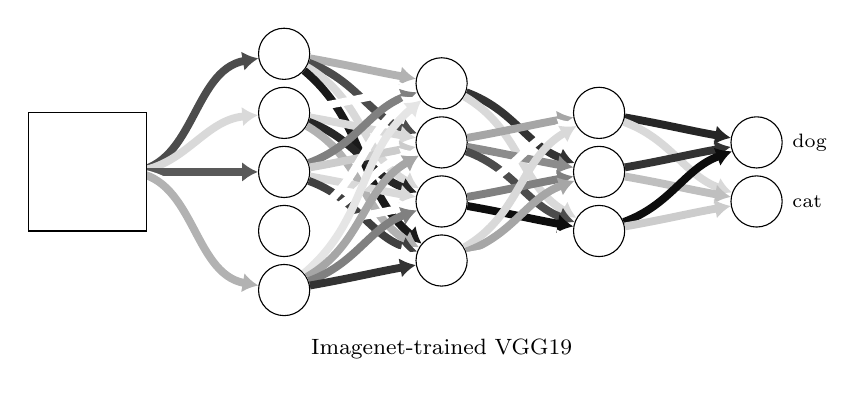
\begin{tikzpicture}
						\node[] at (4.5, -2.25) {\footnotesize{Imagenet-trained VGG19}};
						\node[circle,draw=black, fill=white, minimum size=0.65cm, inner sep=2pt] (n00) at (2.5,1.5) {};
						\node[circle,draw=black, fill=white, minimum size=0.65cm, inner sep=2pt] (n01) at (2.5,0.75) {};
						\node[circle,draw=black, fill=white, minimum size=0.65cm, inner sep=2pt] (n02) at (2.5,0) {};
						\node[circle,draw=black, fill=white, minimum size=0.65cm, inner sep=2pt] (n03) at (2.5,-0.75) {};
						\node[circle,draw=black, fill=white, minimum size=0.65cm, inner sep=2pt] (n04) at (2.5,-1.5) {};
						
						\node[circle,draw=black, fill=white, minimum size=0.65cm, inner sep=2pt] (n10) at (4.5,1.125) {};
						\node[circle,draw=black, fill=white, minimum size=0.65cm, inner sep=2pt] (n11) at (4.5,0.375) {};
						\node[circle,draw=black, fill=white, minimum size=0.65cm, inner sep=2pt] (n12) at (4.5,-0.375) {};
						\node[circle,draw=black, fill=white, minimum size=0.65cm, inner sep=2pt] (n13) at (4.5,-1.125) {};
						
						\node[circle,draw=black, fill=white, minimum size=0.65cm, inner sep=2pt] (n20) at (6.5,0.75) {};
						\node[circle,draw=black, fill=white, minimum size=0.65cm, inner sep=2pt] (n21) at (6.5,0) {};
						\node[circle,draw=black, fill=white, minimum size=0.65cm, inner sep=2pt] (n22) at (6.5,-0.75) {};
						
						\node[circle,draw=black!, fill=white, minimum size=0.65cm, inner sep=2pt, label=right:{\scriptsize{dog}}] (n31) at (8.5,0.375) {};
						\node[circle,draw=black, fill=white, minimum size=0.65cm, inner sep=2pt, label=right:{\scriptsize{cat}}] (n32) at (8.5,-0.375) {};
						
						\draw[color=black!70,-{Latex[length=0.2cm, width=0.25cm]},line width=0.1cm] (0.5,0) to [out=0,in=190] (n00) {};
						\draw[color=black!15,-{Latex[length=0.2cm, width=0.25cm]},line width=0.1cm] (0.5,0) to [out=0,in=185] (n01) {};
						\draw[color=black!65,-{Latex[length=0.2cm, width=0.25cm]},line width=0.1cm] (0.5,0) to [out=0,in=180] (n02) {};
						\draw[color=white,-{Latex[length=0.2cm, width=0.25cm]},line width=0.1cm] (0.5,0) to [out=0,in=175] (n03) {};
						\draw[color=black!30,-{Latex[length=0.2cm, width=0.25cm]},line width=0.1cm] (0.5,0) to [out=0,in=170] (n04) {};
						
						\node[minimum width=1.5cm, minimum height=1.5cm, inner sep=0pt, draw=black, fill=white] at (0,0) {};
						
						\draw[color=black!30,-{Latex[length=0.2cm, width=0.25cm]},line width=0.1cm] (n00) to [out=-10,in=170] (n10) {};
						\draw[color=black!70,-{Latex[length=0.2cm, width=0.25cm]},line width=0.1cm] (n00) to [out=-20,in=160] (n11) {};
						\draw[color=black!15,-{Latex[length=0.2cm, width=0.25cm]},line width=0.1cm] (n00) to [out=-30,in=150] (n12) {};
						\draw[color=black!90,-{Latex[length=0.2cm, width=0.25cm]},line width=0.1cm] (n00) to [out=-40,in=140] (n13) {};
						
						\draw[color=white,-{Latex[length=0.2cm, width=0.25cm]},line width=0.1cm] (n01) to [out=10,in=190] (n10) {};
						\draw[color=black!15,-{Latex[length=0.2cm, width=0.25cm]},line width=0.1cm] (n01) to [out=-10,in=170] (n11) {};
						\draw[color=black!85,-{Latex[length=0.2cm, width=0.25cm]},line width=0.1cm] (n01) to [out=-20,in=160] (n12) {};
						\draw[color=black!30,-{Latex[length=0.2cm, width=0.25cm]},line width=0.1cm] (n01) to [out=-30,in=150] (n13) {};
						
						\draw[color=black!50,-{Latex[length=0.2cm, width=0.25cm]},line width=0.1cm] (n02) to [out=20,in=200] (n10) {};
						\draw[color=black!20,-{Latex[length=0.2cm, width=0.25cm]},line width=0.1cm] (n02) to [out=10,in=190] (n11) {};
						\draw[color=black!15,-{Latex[length=0.2cm, width=0.25cm]},line width=0.1cm] (n02) to [out=-10,in=170] (n12) {};
						\draw[color=black!75,-{Latex[length=0.2cm, width=0.25cm]},line width=0.1cm] (n02) to [out=-20,in=160] (n13) {};
						
						\draw[color=white,-{Latex[length=0.2cm, width=0.25cm]},line width=0.1cm] (n03) to [out=30,in=210] (n10) {};
						\draw[color=white,-{Latex[length=0.2cm, width=0.25cm]},line width=0.1cm] (n03) to [out=20,in=200] (n11) {};
						\draw[color=white,-{Latex[length=0.2cm, width=0.25cm]},line width=0.1cm] (n03) to [out=10,in=190] (n12) {};
						\draw[color=white,-{Latex[length=0.2cm, width=0.25cm]},line width=0.1cm] (n03) to [out=-10,in=170] (n13) {};
						
						\draw[color=black!10,-{Latex[length=0.2cm, width=0.25cm]},line width=0.1cm] (n04) to [out=40,in=220] (n10) {};
						\draw[color=black!35,-{Latex[length=0.2cm, width=0.25cm]},line width=0.1cm] (n04) to [out=30,in=210] (n11) {};
						\draw[color=black!50,-{Latex[length=0.2cm, width=0.25cm]},line width=0.1cm] (n04) to [out=20,in=200] (n12) {};
						\draw[color=black!80,-{Latex[length=0.2cm, width=0.25cm]},line width=0.1cm] (n04) to [out=10,in=190] (n13) {};
						
						\draw[color=white,-{Latex[length=0.2cm, width=0.25cm]},line width=0.1cm] (n10) to [out=-10,in=170] (n20) {};
						\draw[color=black!80,-{Latex[length=0.2cm, width=0.25cm]},line width=0.1cm] (n10) to [out=-20,in=160] (n21) {};
						\draw[color=black!15,-{Latex[length=0.2cm, width=0.25cm]},line width=0.1cm] (n10) to [out=-30,in=150] (n22) {};
						
						\draw[color=black!35,-{Latex[length=0.2cm, width=0.25cm]},line width=0.1cm] (n11) to [out=10,in=190] (n20) {};
						\draw[color=black!45,-{Latex[length=0.2cm, width=0.25cm]},line width=0.1cm] (n11) to [out=-10,in=170] (n21) {};
						\draw[color=black!70,-{Latex[length=0.2cm, width=0.25cm]},line width=0.1cm] (n11) to [out=-20,in=160] (n22) {};
						
						\draw[color=white,-{Latex[length=0.2cm, width=0.25cm]},line width=0.1cm] (n12) to [out=20,in=200] (n20) {};
						\draw[color=black!50,-{Latex[length=0.2cm, width=0.25cm]},line width=0.1cm] (n12) to [out=10,in=190] (n21) {};
						\draw[color=black!95,-{Latex[length=0.2cm, width=0.25cm]},line width=0.1cm] (n12) to [out=-10,in=170] (n22) {};
						
						\draw[color=black!15,-{Latex[length=0.2cm, width=0.25cm]},line width=0.1cm] (n13) to [out=30,in=210] (n20) {};
						\draw[color=black!35,-{Latex[length=0.2cm, width=0.25cm]},line width=0.1cm] (n13) to [out=20,in=200] (n21) {};
						\draw[color=white,-{Latex[length=0.2cm, width=0.25cm]},line width=0.1cm] (n13) to [out=10,in=190] (n22) {};
						
						\draw[color=black!85,-{Latex[length=0.2cm, width=0.25cm]},line width=0.1cm] (n20) to [out=-10,in=170] (n31) {};
						\draw[color=black!15,-{Latex[length=0.2cm, width=0.25cm]},line width=0.1cm] (n20) to [out=-20,in=160] (n32) {};
						
						\draw[color=black!80,-{Latex[length=0.2cm, width=0.25cm]},line width=0.1cm] (n21) to [out=10,in=190] (n31) {};
						\draw[color=black!25,-{Latex[length=0.2cm, width=0.25cm]},line width=0.1cm] (n21) to [out=-10,in=170] (n32) {};
						
						\draw[color=black!95,-{Latex[length=0.2cm, width=0.25cm]},line width=0.1cm] (n22) to [out=20,in=200] (n31) {};
						\draw[color=black!20,-{Latex[length=0.2cm, width=0.25cm]},line width=0.1cm] (n22) to [out=10,in=190] (n32) {};
						
					\end{tikzpicture}
				\end{figure}
			\end{center}
		\end{frame}
	}
	
	\begin{frame}[t]{Explainable AI: Layerwise Relevance Propagation} % 2D CNN with image
		\vspace{1.5cm}
		\begin{center}
			\begin{figure}[t]
				\begin{tikzpicture}
					\node[circle,draw=black, fill=white, minimum size=0.65cm, inner sep=2pt] (n00) at (2.5,1.5) {};
					\node[circle,draw=black, fill=white, minimum size=0.65cm, inner sep=2pt] (n01) at (2.5,0.75) {};
					\node[circle,draw=black, fill=white, minimum size=0.65cm, inner sep=2pt] (n02) at (2.5,0) {};
					\node[circle,draw=black, fill=white, minimum size=0.65cm, inner sep=2pt] (n03) at (2.5,-0.75) {};
					\node[circle,draw=black, fill=white, minimum size=0.65cm, inner sep=2pt] (n04) at (2.5,-1.5) {};
					
					\node[circle,draw=black, fill=white, minimum size=0.65cm, inner sep=2pt] (n10) at (4.5,1.125) {};
					\node[circle,draw=black, fill=white, minimum size=0.65cm, inner sep=2pt] (n11) at (4.5,0.375) {};
					\node[circle,draw=black, fill=white, minimum size=0.65cm, inner sep=2pt] (n12) at (4.5,-0.375) {};
					\node[circle,draw=black, fill=white, minimum size=0.65cm, inner sep=2pt] (n13) at (4.5,-1.125) {};
					
					\node[circle,draw=black, fill=white, minimum size=0.65cm, inner sep=2pt] (n20) at (6.5,0.75) {};
					\node[circle,draw=black, fill=white, minimum size=0.65cm, inner sep=2pt] (n21) at (6.5,0) {};
					\node[circle,draw=black, fill=white, minimum size=0.65cm, inner sep=2pt] (n22) at (6.5,-0.75) {};
					
					\node[circle,draw=black!, fill=white, minimum size=0.65cm, inner sep=2pt, label=right:{\scriptsize{dog}}] (n31) at (8.5,0.375) {};
					\node[circle,draw=black, fill=white, minimum size=0.65cm, inner sep=2pt, label=right:{\scriptsize{cat}}] (n32) at (8.5,-0.375) {};
					
					\draw[color=black!70,-{Latex[length=0.2cm, width=0.25cm]},line width=0.1cm] (0.5,0) to [out=0,in=190] (n00) {};
					\draw[color=black!15,-{Latex[length=0.2cm, width=0.25cm]},line width=0.1cm] (0.5,0) to [out=0,in=185] (n01) {};
					\draw[color=black!65,-{Latex[length=0.2cm, width=0.25cm]},line width=0.1cm] (0.5,0) to [out=0,in=180] (n02) {};
					\draw[color=white,-{Latex[length=0.2cm, width=0.25cm]},line width=0.1cm] (0.5,0) to [out=0,in=175] (n03) {};
					\draw[color=black!30,-{Latex[length=0.2cm, width=0.25cm]},line width=0.1cm] (0.5,0) to [out=0,in=170] (n04) {};
					
					\node[inner sep=0pt, draw=black] at (0,0) {
						\includegraphics[width=1.5cm]{data/dog.png}
					};
					
					\draw[color=black!30,-{Latex[length=0.2cm, width=0.25cm]},line width=0.1cm] (n00) to [out=-10,in=170] (n10) {};
					\draw[color=black!70,-{Latex[length=0.2cm, width=0.25cm]},line width=0.1cm] (n00) to [out=-20,in=160] (n11) {};
					\draw[color=black!15,-{Latex[length=0.2cm, width=0.25cm]},line width=0.1cm] (n00) to [out=-30,in=150] (n12) {};
					\draw[color=black!90,-{Latex[length=0.2cm, width=0.25cm]},line width=0.1cm] (n00) to [out=-40,in=140] (n13) {};
					
					\draw[color=white,-{Latex[length=0.2cm, width=0.25cm]},line width=0.1cm] (n01) to [out=10,in=190] (n10) {};
					\draw[color=black!15,-{Latex[length=0.2cm, width=0.25cm]},line width=0.1cm] (n01) to [out=-10,in=170] (n11) {};
					\draw[color=black!85,-{Latex[length=0.2cm, width=0.25cm]},line width=0.1cm] (n01) to [out=-20,in=160] (n12) {};
					\draw[color=black!30,-{Latex[length=0.2cm, width=0.25cm]},line width=0.1cm] (n01) to [out=-30,in=150] (n13) {};
					
					\draw[color=black!50,-{Latex[length=0.2cm, width=0.25cm]},line width=0.1cm] (n02) to [out=20,in=200] (n10) {};
					\draw[color=black!20,-{Latex[length=0.2cm, width=0.25cm]},line width=0.1cm] (n02) to [out=10,in=190] (n11) {};
					\draw[color=black!15,-{Latex[length=0.2cm, width=0.25cm]},line width=0.1cm] (n02) to [out=-10,in=170] (n12) {};
					\draw[color=black!75,-{Latex[length=0.2cm, width=0.25cm]},line width=0.1cm] (n02) to [out=-20,in=160] (n13) {};
					
					\draw[color=white,-{Latex[length=0.2cm, width=0.25cm]},line width=0.1cm] (n03) to [out=30,in=210] (n10) {};
					\draw[color=white,-{Latex[length=0.2cm, width=0.25cm]},line width=0.1cm] (n03) to [out=20,in=200] (n11) {};
					\draw[color=white,-{Latex[length=0.2cm, width=0.25cm]},line width=0.1cm] (n03) to [out=10,in=190] (n12) {};
					\draw[color=white,-{Latex[length=0.2cm, width=0.25cm]},line width=0.1cm] (n03) to [out=-10,in=170] (n13) {};
					
					\draw[color=black!10,-{Latex[length=0.2cm, width=0.25cm]},line width=0.1cm] (n04) to [out=40,in=220] (n10) {};
					\draw[color=black!35,-{Latex[length=0.2cm, width=0.25cm]},line width=0.1cm] (n04) to [out=30,in=210] (n11) {};
					\draw[color=black!50,-{Latex[length=0.2cm, width=0.25cm]},line width=0.1cm] (n04) to [out=20,in=200] (n12) {};
					\draw[color=black!80,-{Latex[length=0.2cm, width=0.25cm]},line width=0.1cm] (n04) to [out=10,in=190] (n13) {};
					
					\draw[color=white,-{Latex[length=0.2cm, width=0.25cm]},line width=0.1cm] (n10) to [out=-10,in=170] (n20) {};
					\draw[color=black!80,-{Latex[length=0.2cm, width=0.25cm]},line width=0.1cm] (n10) to [out=-20,in=160] (n21) {};
					\draw[color=black!15,-{Latex[length=0.2cm, width=0.25cm]},line width=0.1cm] (n10) to [out=-30,in=150] (n22) {};
					
					\draw[color=black!35,-{Latex[length=0.2cm, width=0.25cm]},line width=0.1cm] (n11) to [out=10,in=190] (n20) {};
					\draw[color=black!45,-{Latex[length=0.2cm, width=0.25cm]},line width=0.1cm] (n11) to [out=-10,in=170] (n21) {};
					\draw[color=black!70,-{Latex[length=0.2cm, width=0.25cm]},line width=0.1cm] (n11) to [out=-20,in=160] (n22) {};
					
					\draw[color=white,-{Latex[length=0.2cm, width=0.25cm]},line width=0.1cm] (n12) to [out=20,in=200] (n20) {};
					\draw[color=black!50,-{Latex[length=0.2cm, width=0.25cm]},line width=0.1cm] (n12) to [out=10,in=190] (n21) {};
					\draw[color=black!95,-{Latex[length=0.2cm, width=0.25cm]},line width=0.1cm] (n12) to [out=-10,in=170] (n22) {};
					
					\draw[color=black!15,-{Latex[length=0.2cm, width=0.25cm]},line width=0.1cm] (n13) to [out=30,in=210] (n20) {};
					\draw[color=black!35,-{Latex[length=0.2cm, width=0.25cm]},line width=0.1cm] (n13) to [out=20,in=200] (n21) {};
					\draw[color=white,-{Latex[length=0.2cm, width=0.25cm]},line width=0.1cm] (n13) to [out=10,in=190] (n22) {};
					
					\draw[color=black!85,-{Latex[length=0.2cm, width=0.25cm]},line width=0.1cm] (n20) to [out=-10,in=170] (n31) {};
					\draw[color=black!15,-{Latex[length=0.2cm, width=0.25cm]},line width=0.1cm] (n20) to [out=-20,in=160] (n32) {};
					
					\draw[color=black!80,-{Latex[length=0.2cm, width=0.25cm]},line width=0.1cm] (n21) to [out=10,in=190] (n31) {};
					\draw[color=black!25,-{Latex[length=0.2cm, width=0.25cm]},line width=0.1cm] (n21) to [out=-10,in=170] (n32) {};
					
					\draw[color=black!95,-{Latex[length=0.2cm, width=0.25cm]},line width=0.1cm] (n22) to [out=20,in=200] (n31) {};
					\draw[color=black!20,-{Latex[length=0.2cm, width=0.25cm]},line width=0.1cm] (n22) to [out=10,in=190] (n32) {};
					
				\end{tikzpicture}
			\end{figure}
		\end{center}
	\end{frame}
	
	\begin{frame}[t]{Explainable AI: Layerwise Relevance Propagation} % 2D CNN first layer
		\vspace{1.5cm}
		\begin{center}
			\begin{figure}
				\begin{tikzpicture}
					\node[circle,draw=black!70, fill=black!70, minimum size=0.65cm, inner sep=2pt] (n00) at (2.5,1.5) {\textcolor{white}{\tiny{0.70}}};
					\node[circle,draw=black!15, fill=black!15, minimum size=0.65cm, inner sep=2pt] (n01) at (2.5,0.75) {\tiny{0.15}};
					\node[circle,draw=black!65, fill=black!65, minimum size=0.65cm, inner sep=2pt] (n02) at (2.5,0) {\textcolor{white}{\tiny{0.65}}};
					\node[circle,draw=white, fill=white, minimum size=0.65cm, inner sep=2pt] (n03) at (2.5,-0.75) {};
					\node[circle,draw=black!30, fill=black!30, minimum size=0.65cm, inner sep=2pt] (n04) at (2.5,-1.5) {\tiny{0.30}};
					
					\node[circle,draw=black, fill=white, minimum size=0.65cm, inner sep=2pt] (n10) at (4.5,1.125) {};
					\node[circle,draw=black, fill=white, minimum size=0.65cm, inner sep=2pt] (n11) at (4.5,0.375) {};
					\node[circle,draw=black, fill=white, minimum size=0.65cm, inner sep=2pt] (n12) at (4.5,-0.375) {};
					\node[circle,draw=black, fill=white, minimum size=0.65cm, inner sep=2pt] (n13) at (4.5,-1.125) {};
					
					\node[circle,draw=black, fill=white, minimum size=0.65cm, inner sep=2pt] (n20) at (6.5,0.75) {};
					\node[circle,draw=black, fill=white, minimum size=0.65cm, inner sep=2pt] (n21) at (6.5,0) {};
					\node[circle,draw=black, fill=white, minimum size=0.65cm, inner sep=2pt] (n22) at (6.5,-0.75) {};
					
					\node[circle,draw=black!, fill=white, minimum size=0.65cm, inner sep=2pt, label=right:{\scriptsize{dog}}] (n31) at (8.5,0.375) {};
					\node[circle,draw=black, fill=white, minimum size=0.65cm, inner sep=2pt, label=right:{\scriptsize{cat}}] (n32) at (8.5,-0.375) {};
					
					\draw[color=black!70,-{Latex[length=0.2cm, width=0.25cm]},line width=0.1cm] (0.5,0) to [out=0,in=190] (n00) {};
					\draw[color=black!15,-{Latex[length=0.2cm, width=0.25cm]},line width=0.1cm] (0.5,0) to [out=0,in=185] (n01) {};
					\draw[color=black!65,-{Latex[length=0.2cm, width=0.25cm]},line width=0.1cm] (0.5,0) to [out=0,in=180] (n02) {};
					\draw[color=white,-{Latex[length=0.2cm, width=0.25cm]},line width=0.1cm] (0.5,0) to [out=0,in=175] (n03) {};
					\draw[color=black!30,-{Latex[length=0.2cm, width=0.25cm]},line width=0.1cm] (0.5,0) to [out=0,in=170] (n04) {};
					
					\node[inner sep=0pt, draw=black] at (0,0) {
						\includegraphics[width=1.5cm]{data/dog.png}
					};
					
					\draw[color=black!30,-{Latex[length=0.2cm, width=0.25cm]},line width=0.1cm] (n00) to [out=-10,in=170] (n10) {};
					\draw[color=black!70,-{Latex[length=0.2cm, width=0.25cm]},line width=0.1cm] (n00) to [out=-20,in=160] (n11) {};
					\draw[color=black!15,-{Latex[length=0.2cm, width=0.25cm]},line width=0.1cm] (n00) to [out=-30,in=150] (n12) {};
					\draw[color=black!90,-{Latex[length=0.2cm, width=0.25cm]},line width=0.1cm] (n00) to [out=-40,in=140] (n13) {};
					
					\draw[color=white,-{Latex[length=0.2cm, width=0.25cm]},line width=0.1cm] (n01) to [out=10,in=190] (n10) {};
					\draw[color=black!15,-{Latex[length=0.2cm, width=0.25cm]},line width=0.1cm] (n01) to [out=-10,in=170] (n11) {};
					\draw[color=black!85,-{Latex[length=0.2cm, width=0.25cm]},line width=0.1cm] (n01) to [out=-20,in=160] (n12) {};
					\draw[color=black!30,-{Latex[length=0.2cm, width=0.25cm]},line width=0.1cm] (n01) to [out=-30,in=150] (n13) {};
					
					\draw[color=black!50,-{Latex[length=0.2cm, width=0.25cm]},line width=0.1cm] (n02) to [out=20,in=200] (n10) {};
					\draw[color=black!20,-{Latex[length=0.2cm, width=0.25cm]},line width=0.1cm] (n02) to [out=10,in=190] (n11) {};
					\draw[color=black!15,-{Latex[length=0.2cm, width=0.25cm]},line width=0.1cm] (n02) to [out=-10,in=170] (n12) {};
					\draw[color=black!75,-{Latex[length=0.2cm, width=0.25cm]},line width=0.1cm] (n02) to [out=-20,in=160] (n13) {};
					
					\draw[color=white,-{Latex[length=0.2cm, width=0.25cm]},line width=0.1cm] (n03) to [out=30,in=210] (n10) {};
					\draw[color=white,-{Latex[length=0.2cm, width=0.25cm]},line width=0.1cm] (n03) to [out=20,in=200] (n11) {};
					\draw[color=white,-{Latex[length=0.2cm, width=0.25cm]},line width=0.1cm] (n03) to [out=10,in=190] (n12) {};
					\draw[color=white,-{Latex[length=0.2cm, width=0.25cm]},line width=0.1cm] (n03) to [out=-10,in=170] (n13) {};
					
					\draw[color=black!10,-{Latex[length=0.2cm, width=0.25cm]},line width=0.1cm] (n04) to [out=40,in=220] (n10) {};
					\draw[color=black!35,-{Latex[length=0.2cm, width=0.25cm]},line width=0.1cm] (n04) to [out=30,in=210] (n11) {};
					\draw[color=black!50,-{Latex[length=0.2cm, width=0.25cm]},line width=0.1cm] (n04) to [out=20,in=200] (n12) {};
					\draw[color=black!80,-{Latex[length=0.2cm, width=0.25cm]},line width=0.1cm] (n04) to [out=10,in=190] (n13) {};
					
					\draw[color=white,-{Latex[length=0.2cm, width=0.25cm]},line width=0.1cm] (n10) to [out=-10,in=170] (n20) {};
					\draw[color=black!80,-{Latex[length=0.2cm, width=0.25cm]},line width=0.1cm] (n10) to [out=-20,in=160] (n21) {};
					\draw[color=black!15,-{Latex[length=0.2cm, width=0.25cm]},line width=0.1cm] (n10) to [out=-30,in=150] (n22) {};
					
					\draw[color=black!35,-{Latex[length=0.2cm, width=0.25cm]},line width=0.1cm] (n11) to [out=10,in=190] (n20) {};
					\draw[color=black!45,-{Latex[length=0.2cm, width=0.25cm]},line width=0.1cm] (n11) to [out=-10,in=170] (n21) {};
					\draw[color=black!70,-{Latex[length=0.2cm, width=0.25cm]},line width=0.1cm] (n11) to [out=-20,in=160] (n22) {};
					
					\draw[color=white,-{Latex[length=0.2cm, width=0.25cm]},line width=0.1cm] (n12) to [out=20,in=200] (n20) {};
					\draw[color=black!50,-{Latex[length=0.2cm, width=0.25cm]},line width=0.1cm] (n12) to [out=10,in=190] (n21) {};
					\draw[color=black!95,-{Latex[length=0.2cm, width=0.25cm]},line width=0.1cm] (n12) to [out=-10,in=170] (n22) {};
					
					\draw[color=black!15,-{Latex[length=0.2cm, width=0.25cm]},line width=0.1cm] (n13) to [out=30,in=210] (n20) {};
					\draw[color=black!35,-{Latex[length=0.2cm, width=0.25cm]},line width=0.1cm] (n13) to [out=20,in=200] (n21) {};
					\draw[color=white,-{Latex[length=0.2cm, width=0.25cm]},line width=0.1cm] (n13) to [out=10,in=190] (n22) {};
					
					\draw[color=black!85,-{Latex[length=0.2cm, width=0.25cm]},line width=0.1cm] (n20) to [out=-10,in=170] (n31) {};
					\draw[color=black!15,-{Latex[length=0.2cm, width=0.25cm]},line width=0.1cm] (n20) to [out=-20,in=160] (n32) {};
					
					\draw[color=black!80,-{Latex[length=0.2cm, width=0.25cm]},line width=0.1cm] (n21) to [out=10,in=190] (n31) {};
					\draw[color=black!25,-{Latex[length=0.2cm, width=0.25cm]},line width=0.1cm] (n21) to [out=-10,in=170] (n32) {};
					
					\draw[color=black!95,-{Latex[length=0.2cm, width=0.25cm]},line width=0.1cm] (n22) to [out=20,in=200] (n31) {};
					\draw[color=black!20,-{Latex[length=0.2cm, width=0.25cm]},line width=0.1cm] (n22) to [out=10,in=190] (n32) {};
					
				\end{tikzpicture}
			\end{figure}
		\end{center}
	\end{frame}
	
	\begin{frame}[t]{Explainable AI: Layerwise Relevance Propagation} % 2D CNN highlighted node
		\vspace{1.5cm}
		\begin{center}
			\begin{figure}
				\begin{tikzpicture}
					\node[circle,draw=black!70, fill=black!70, minimum size=0.65cm, inner sep=2pt] (n00) at (2.5,1.5) {\textcolor{white}{\tiny{0.70}}};
					\node[circle,draw=black!15, fill=black!15, minimum size=0.65cm, inner sep=2pt] (n01) at (2.5,0.75) {\tiny{0.15}};
					\node[circle,draw=black!65, fill=black!65, minimum size=0.65cm, inner sep=2pt] (n02) at (2.5,0) {\textcolor{white}{\tiny{0.65}}};
					\node[circle,draw=white, fill=white, minimum size=0.65cm, inner sep=2pt] (n03) at (2.5,-0.75) {};
					\node[circle,draw=black!30, fill=black!30, minimum size=0.65cm, inner sep=2pt] (n04) at (2.5,-1.5) {\tiny{0.30}};
					
					\node[circle,draw=red, fill=red!20, minimum size=0.65cm, inner sep=2pt,label=\tiny{$v_{1,0}$}] (n10) at (4.5,1.125) {};
					\node[circle,draw=black, fill=white, minimum size=0.65cm, inner sep=2pt] (n11) at (4.5,0.375) {};
					\node[circle,draw=black, fill=white, minimum size=0.65cm, inner sep=2pt] (n12) at (4.5,-0.375) {};
					\node[circle,draw=black, fill=white, minimum size=0.65cm, inner sep=2pt] (n13) at (4.5,-1.125) {};
					
					\node[circle,draw=black, fill=white, minimum size=0.65cm, inner sep=2pt] (n20) at (6.5,0.75) {};
					\node[circle,draw=black, fill=white, minimum size=0.65cm, inner sep=2pt] (n21) at (6.5,0) {};
					\node[circle,draw=black, fill=white, minimum size=0.65cm, inner sep=2pt] (n22) at (6.5,-0.75) {};
					
					\node[circle,draw=black!, fill=white, minimum size=0.65cm, inner sep=2pt, label=right:{\scriptsize{dog}}] (n31) at (8.5,0.375) {};
					\node[circle,draw=black, fill=white, minimum size=0.65cm, inner sep=2pt, label=right:{\scriptsize{cat}}] (n32) at (8.5,-0.375) {};
					
					\draw[color=black!70,-{Latex[length=0.2cm, width=0.25cm]},line width=0.1cm] (0.5,0) to [out=0,in=190] (n00) {};
					\draw[color=black!15,-{Latex[length=0.2cm, width=0.25cm]},line width=0.1cm] (0.5,0) to [out=0,in=185] (n01) {};
					\draw[color=black!65,-{Latex[length=0.2cm, width=0.25cm]},line width=0.1cm] (0.5,0) to [out=0,in=180] (n02) {};
					\draw[color=white,-{Latex[length=0.2cm, width=0.25cm]},line width=0.1cm] (0.5,0) to [out=0,in=175] (n03) {};
					\draw[color=black!30,-{Latex[length=0.2cm, width=0.25cm]},line width=0.1cm] (0.5,0) to [out=0,in=170] (n04) {};
					
					\node[inner sep=0pt, draw=black] at (0,0) {
						\includegraphics[width=1.5cm]{data/dog.png}
					};
					
					\draw[color=black!30,-{Latex[length=0.2cm, width=0.25cm]},line width=0.1cm] (n00) to [out=-10,in=170] (n10) {};
					\draw[color=black!70,-{Latex[length=0.2cm, width=0.25cm]},line width=0.1cm] (n00) to [out=-20,in=160] (n11) {};
					\draw[color=black!15,-{Latex[length=0.2cm, width=0.25cm]},line width=0.1cm] (n00) to [out=-30,in=150] (n12) {};
					\draw[color=black!90,-{Latex[length=0.2cm, width=0.25cm]},line width=0.1cm] (n00) to [out=-40,in=140] (n13) {};
					
					\draw[color=white,-{Latex[length=0.2cm, width=0.25cm]},line width=0.1cm] (n01) to [out=10,in=190] (n10) {};
					\draw[color=black!15,-{Latex[length=0.2cm, width=0.25cm]},line width=0.1cm] (n01) to [out=-10,in=170] (n11) {};
					\draw[color=black!85,-{Latex[length=0.2cm, width=0.25cm]},line width=0.1cm] (n01) to [out=-20,in=160] (n12) {};
					\draw[color=black!30,-{Latex[length=0.2cm, width=0.25cm]},line width=0.1cm] (n01) to [out=-30,in=150] (n13) {};
					
					\draw[color=black!50,-{Latex[length=0.2cm, width=0.25cm]},line width=0.1cm] (n02) to [out=20,in=200] (n10) {};
					\draw[color=black!20,-{Latex[length=0.2cm, width=0.25cm]},line width=0.1cm] (n02) to [out=10,in=190] (n11) {};
					\draw[color=black!15,-{Latex[length=0.2cm, width=0.25cm]},line width=0.1cm] (n02) to [out=-10,in=170] (n12) {};
					\draw[color=black!75,-{Latex[length=0.2cm, width=0.25cm]},line width=0.1cm] (n02) to [out=-20,in=160] (n13) {};
					
					\draw[color=white,-{Latex[length=0.2cm, width=0.25cm]},line width=0.1cm] (n03) to [out=30,in=210] (n10) {};
					\draw[color=white,-{Latex[length=0.2cm, width=0.25cm]},line width=0.1cm] (n03) to [out=20,in=200] (n11) {};
					\draw[color=white,-{Latex[length=0.2cm, width=0.25cm]},line width=0.1cm] (n03) to [out=10,in=190] (n12) {};
					\draw[color=white,-{Latex[length=0.2cm, width=0.25cm]},line width=0.1cm] (n03) to [out=-10,in=170] (n13) {};
					
					\draw[color=black!10,-{Latex[length=0.2cm, width=0.25cm]},line width=0.1cm] (n04) to [out=40,in=220] (n10) {};
					\draw[color=black!35,-{Latex[length=0.2cm, width=0.25cm]},line width=0.1cm] (n04) to [out=30,in=210] (n11) {};
					\draw[color=black!50,-{Latex[length=0.2cm, width=0.25cm]},line width=0.1cm] (n04) to [out=20,in=200] (n12) {};
					\draw[color=black!80,-{Latex[length=0.2cm, width=0.25cm]},line width=0.1cm] (n04) to [out=10,in=190] (n13) {};
					
					\draw[color=white,-{Latex[length=0.2cm, width=0.25cm]},line width=0.1cm] (n10) to [out=-10,in=170] (n20) {};
					\draw[color=black!80,-{Latex[length=0.2cm, width=0.25cm]},line width=0.1cm] (n10) to [out=-20,in=160] (n21) {};
					\draw[color=black!15,-{Latex[length=0.2cm, width=0.25cm]},line width=0.1cm] (n10) to [out=-30,in=150] (n22) {};
					
					\draw[color=black!35,-{Latex[length=0.2cm, width=0.25cm]},line width=0.1cm] (n11) to [out=10,in=190] (n20) {};
					\draw[color=black!45,-{Latex[length=0.2cm, width=0.25cm]},line width=0.1cm] (n11) to [out=-10,in=170] (n21) {};
					\draw[color=black!70,-{Latex[length=0.2cm, width=0.25cm]},line width=0.1cm] (n11) to [out=-20,in=160] (n22) {};
					
					\draw[color=white,-{Latex[length=0.2cm, width=0.25cm]},line width=0.1cm] (n12) to [out=20,in=200] (n20) {};
					\draw[color=black!50,-{Latex[length=0.2cm, width=0.25cm]},line width=0.1cm] (n12) to [out=10,in=190] (n21) {};
					\draw[color=black!95,-{Latex[length=0.2cm, width=0.25cm]},line width=0.1cm] (n12) to [out=-10,in=170] (n22) {};
					
					\draw[color=black!15,-{Latex[length=0.2cm, width=0.25cm]},line width=0.1cm] (n13) to [out=30,in=210] (n20) {};
					\draw[color=black!35,-{Latex[length=0.2cm, width=0.25cm]},line width=0.1cm] (n13) to [out=20,in=200] (n21) {};
					\draw[color=white,-{Latex[length=0.2cm, width=0.25cm]},line width=0.1cm] (n13) to [out=10,in=190] (n22) {};
					
					\draw[color=black!85,-{Latex[length=0.2cm, width=0.25cm]},line width=0.1cm] (n20) to [out=-10,in=170] (n31) {};
					\draw[color=black!15,-{Latex[length=0.2cm, width=0.25cm]},line width=0.1cm] (n20) to [out=-20,in=160] (n32) {};
					
					\draw[color=black!80,-{Latex[length=0.2cm, width=0.25cm]},line width=0.1cm] (n21) to [out=10,in=190] (n31) {};
					\draw[color=black!25,-{Latex[length=0.2cm, width=0.25cm]},line width=0.1cm] (n21) to [out=-10,in=170] (n32) {};
					
					\draw[color=black!95,-{Latex[length=0.2cm, width=0.25cm]},line width=0.1cm] (n22) to [out=20,in=200] (n31) {};
					\draw[color=black!20,-{Latex[length=0.2cm, width=0.25cm]},line width=0.1cm] (n22) to [out=10,in=190] (n32) {};
					
				\end{tikzpicture}
			\end{figure}
		\end{center}
	\end{frame}
	
	\begin{frame}[t]{Explainable AI: Layerwise Relevance Propagation} % 2D CNN node computation
		\vspace{1.5cm}
		\begin{center}
			\begin{figure}
				\begin{tikzpicture}
					\node[circle,draw=black!70, fill=black!70, minimum size=0.65cm, inner sep=2pt] (n00) at (2.5,1.5) {\textcolor{white}{\tiny{0.70}}};
					\node[circle,draw=black!15, fill=black!15, minimum size=0.65cm, inner sep=2pt] (n01) at (2.5,0.75) {\tiny{0.15}};
					\node[circle,draw=black!65, fill=black!65, minimum size=0.65cm, inner sep=2pt] (n02) at (2.5,0) {\textcolor{white}{\tiny{0.65}}};
					\node[circle,draw=white, fill=white, minimum size=0.65cm, inner sep=2pt] (n03) at (2.5,-0.75) {};
					\node[circle,draw=black!30, fill=black!30, minimum size=0.65cm, inner sep=2pt] (n04) at (2.5,-1.5) {\tiny{0.30}};
					
					\node[circle,draw=red, fill=red!20, minimum size=0.65cm, inner sep=2pt,label=\tiny{$v_{1,0}$}] (n10) at (4.5,1.125) {};
					\node[circle,draw=black, fill=white, minimum size=0.65cm, inner sep=2pt] (n11) at (4.5,0.375) {};
					\node[circle,draw=black, fill=white, minimum size=0.65cm, inner sep=2pt] (n12) at (4.5,-0.375) {};
					\node[circle,draw=black, fill=white, minimum size=0.65cm, inner sep=2pt] (n13) at (4.5,-1.125) {};
					
					\node[circle,draw=black, fill=white, minimum size=0.65cm, inner sep=2pt] (n20) at (6.5,0.75) {};
					\node[circle,draw=black, fill=white, minimum size=0.65cm, inner sep=2pt] (n21) at (6.5,0) {};
					\node[circle,draw=black, fill=white, minimum size=0.65cm, inner sep=2pt] (n22) at (6.5,-0.75) {};
					
					\node[circle,draw=black!, fill=white, minimum size=0.65cm, inner sep=2pt, label=right:{\scriptsize{dog}}] (n31) at (8.5,0.375) {};
					\node[circle,draw=black, fill=white, minimum size=0.65cm, inner sep=2pt, label=right:{\scriptsize{cat}}] (n32) at (8.5,-0.375) {};
					
					\draw[color=black!70,-{Latex[length=0.2cm, width=0.25cm]},line width=0.1cm] (0.5,0) to [out=0,in=190] (n00) {};
					\draw[color=black!15,-{Latex[length=0.2cm, width=0.25cm]},line width=0.1cm] (0.5,0) to [out=0,in=185] (n01) {};
					\draw[color=black!65,-{Latex[length=0.2cm, width=0.25cm]},line width=0.1cm] (0.5,0) to [out=0,in=180] (n02) {};
					\draw[color=white,-{Latex[length=0.2cm, width=0.25cm]},line width=0.1cm] (0.5,0) to [out=0,in=175] (n03) {};
					\draw[color=black!30,-{Latex[length=0.2cm, width=0.25cm]},line width=0.1cm] (0.5,0) to [out=0,in=170] (n04) {};
					
					\node[inner sep=0pt, draw=black] at (0,0) {
						\includegraphics[width=1.5cm]{data/dog.png}
					};
					
					\draw[color=black!30,-{Latex[length=0.2cm, width=0.25cm]},line width=0.1cm] (n00) to [out=-10,in=170] (n10) {};
					\draw[color=black!70,-{Latex[length=0.2cm, width=0.25cm]},line width=0.1cm] (n00) to [out=-20,in=160] (n11) {};
					\draw[color=black!15,-{Latex[length=0.2cm, width=0.25cm]},line width=0.1cm] (n00) to [out=-30,in=150] (n12) {};
					\draw[color=black!90,-{Latex[length=0.2cm, width=0.25cm]},line width=0.1cm] (n00) to [out=-40,in=140] (n13) {};
					
					\draw[color=white,-{Latex[length=0.2cm, width=0.25cm]},line width=0.1cm] (n01) to [out=10,in=190] (n10) {};
					\draw[color=black!15,-{Latex[length=0.2cm, width=0.25cm]},line width=0.1cm] (n01) to [out=-10,in=170] (n11) {};
					\draw[color=black!85,-{Latex[length=0.2cm, width=0.25cm]},line width=0.1cm] (n01) to [out=-20,in=160] (n12) {};
					\draw[color=black!30,-{Latex[length=0.2cm, width=0.25cm]},line width=0.1cm] (n01) to [out=-30,in=150] (n13) {};
					
					\draw[color=black!50,-{Latex[length=0.2cm, width=0.25cm]},line width=0.1cm] (n02) to [out=20,in=200] (n10) {};
					\draw[color=black!20,-{Latex[length=0.2cm, width=0.25cm]},line width=0.1cm] (n02) to [out=10,in=190] (n11) {};
					\draw[color=black!15,-{Latex[length=0.2cm, width=0.25cm]},line width=0.1cm] (n02) to [out=-10,in=170] (n12) {};
					\draw[color=black!75,-{Latex[length=0.2cm, width=0.25cm]},line width=0.1cm] (n02) to [out=-20,in=160] (n13) {};
					
					\draw[color=white,-{Latex[length=0.2cm, width=0.25cm]},line width=0.1cm] (n03) to [out=30,in=210] (n10) {};
					\draw[color=white,-{Latex[length=0.2cm, width=0.25cm]},line width=0.1cm] (n03) to [out=20,in=200] (n11) {};
					\draw[color=white,-{Latex[length=0.2cm, width=0.25cm]},line width=0.1cm] (n03) to [out=10,in=190] (n12) {};
					\draw[color=white,-{Latex[length=0.2cm, width=0.25cm]},line width=0.1cm] (n03) to [out=-10,in=170] (n13) {};
					
					\draw[color=black!10,-{Latex[length=0.2cm, width=0.25cm]},line width=0.1cm] (n04) to [out=40,in=220] (n10) {};
					\draw[color=black!35,-{Latex[length=0.2cm, width=0.25cm]},line width=0.1cm] (n04) to [out=30,in=210] (n11) {};
					\draw[color=black!50,-{Latex[length=0.2cm, width=0.25cm]},line width=0.1cm] (n04) to [out=20,in=200] (n12) {};
					\draw[color=black!80,-{Latex[length=0.2cm, width=0.25cm]},line width=0.1cm] (n04) to [out=10,in=190] (n13) {};
					
					\draw[color=white,-{Latex[length=0.2cm, width=0.25cm]},line width=0.1cm] (n10) to [out=-10,in=170] (n20) {};
					\draw[color=black!80,-{Latex[length=0.2cm, width=0.25cm]},line width=0.1cm] (n10) to [out=-20,in=160] (n21) {};
					\draw[color=black!15,-{Latex[length=0.2cm, width=0.25cm]},line width=0.1cm] (n10) to [out=-30,in=150] (n22) {};
					
					\draw[color=black!35,-{Latex[length=0.2cm, width=0.25cm]},line width=0.1cm] (n11) to [out=10,in=190] (n20) {};
					\draw[color=black!45,-{Latex[length=0.2cm, width=0.25cm]},line width=0.1cm] (n11) to [out=-10,in=170] (n21) {};
					\draw[color=black!70,-{Latex[length=0.2cm, width=0.25cm]},line width=0.1cm] (n11) to [out=-20,in=160] (n22) {};
					
					\draw[color=white,-{Latex[length=0.2cm, width=0.25cm]},line width=0.1cm] (n12) to [out=20,in=200] (n20) {};
					\draw[color=black!50,-{Latex[length=0.2cm, width=0.25cm]},line width=0.1cm] (n12) to [out=10,in=190] (n21) {};
					\draw[color=black!95,-{Latex[length=0.2cm, width=0.25cm]},line width=0.1cm] (n12) to [out=-10,in=170] (n22) {};
					
					\draw[color=black!15,-{Latex[length=0.2cm, width=0.25cm]},line width=0.1cm] (n13) to [out=30,in=210] (n20) {};
					\draw[color=black!35,-{Latex[length=0.2cm, width=0.25cm]},line width=0.1cm] (n13) to [out=20,in=200] (n21) {};
					\draw[color=white,-{Latex[length=0.2cm, width=0.25cm]},line width=0.1cm] (n13) to [out=10,in=190] (n22) {};
					
					\draw[color=black!85,-{Latex[length=0.2cm, width=0.25cm]},line width=0.1cm] (n20) to [out=-10,in=170] (n31) {};
					\draw[color=black!15,-{Latex[length=0.2cm, width=0.25cm]},line width=0.1cm] (n20) to [out=-20,in=160] (n32) {};
					
					\draw[color=black!80,-{Latex[length=0.2cm, width=0.25cm]},line width=0.1cm] (n21) to [out=10,in=190] (n31) {};
					\draw[color=black!25,-{Latex[length=0.2cm, width=0.25cm]},line width=0.1cm] (n21) to [out=-10,in=170] (n32) {};
					
					\draw[color=black!95,-{Latex[length=0.2cm, width=0.25cm]},line width=0.1cm] (n22) to [out=20,in=200] (n31) {};
					\draw[color=black!20,-{Latex[length=0.2cm, width=0.25cm]},line width=0.1cm] (n22) to [out=10,in=190] (n32) {};
					
				\end{tikzpicture}
			\end{figure}
			$$v_{1,0}=\sum v_{0,j}*w_{j,1}$$
		\end{center}
	\end{frame}	
	
	\begin{frame}[t]{Explainable AI: Layerwise Relevance Propagation} % 2D CNN node computed
		\vspace{1.5cm}
		\begin{center}
			\begin{figure}
				\begin{tikzpicture}
					\node[circle,draw=black!70, fill=black!70, minimum size=0.65cm, inner sep=2pt] (n00) at (2.5,1.5) {\textcolor{white}{\tiny{0.70}}};
					\node[circle,draw=black!15, fill=black!15, minimum size=0.65cm, inner sep=2pt] (n01) at (2.5,0.75) {\tiny{0.15}};
					\node[circle,draw=black!65, fill=black!65, minimum size=0.65cm, inner sep=2pt] (n02) at (2.5,0) {\textcolor{white}{\tiny{0.65}}};
					\node[circle,draw=white, fill=white, minimum size=0.65cm, inner sep=2pt] (n03) at (2.5,-0.75) {};
					\node[circle,draw=black!30, fill=black!30, minimum size=0.65cm, inner sep=2pt] (n04) at (2.5,-1.5) {\tiny{0.30}};
					
					\node[circle,draw=black!35, fill=black!35, minimum size=0.65cm, inner sep=2pt] (n10) at (4.5,1.125) {\tiny{0.35}};
					\node[circle,draw=black, fill=white, minimum size=0.65cm, inner sep=2pt] (n11) at (4.5,0.375) {};
					\node[circle,draw=black, fill=white, minimum size=0.65cm, inner sep=2pt] (n12) at (4.5,-0.375) {};
					\node[circle,draw=black, fill=white, minimum size=0.65cm, inner sep=2pt] (n13) at (4.5,-1.125) {};
					
					\node[circle,draw=black, fill=white, minimum size=0.65cm, inner sep=2pt] (n20) at (6.5,0.75) {};
					\node[circle,draw=black, fill=white, minimum size=0.65cm, inner sep=2pt] (n21) at (6.5,0) {};
					\node[circle,draw=black, fill=white, minimum size=0.65cm, inner sep=2pt] (n22) at (6.5,-0.75) {};
					
					\node[circle,draw=black!, fill=white, minimum size=0.65cm, inner sep=2pt, label=right:{\scriptsize{dog}}] (n31) at (8.5,0.375) {};
					\node[circle,draw=black, fill=white, minimum size=0.65cm, inner sep=2pt, label=right:{\scriptsize{cat}}] (n32) at (8.5,-0.375) {};
					
					\draw[color=black!70,-{Latex[length=0.2cm, width=0.25cm]},line width=0.1cm] (0.5,0) to [out=0,in=190] (n00) {};
					\draw[color=black!15,-{Latex[length=0.2cm, width=0.25cm]},line width=0.1cm] (0.5,0) to [out=0,in=185] (n01) {};
					\draw[color=black!65,-{Latex[length=0.2cm, width=0.25cm]},line width=0.1cm] (0.5,0) to [out=0,in=180] (n02) {};
					\draw[color=white,-{Latex[length=0.2cm, width=0.25cm]},line width=0.1cm] (0.5,0) to [out=0,in=175] (n03) {};
					\draw[color=black!30,-{Latex[length=0.2cm, width=0.25cm]},line width=0.1cm] (0.5,0) to [out=0,in=170] (n04) {};
					
					\node[inner sep=0pt, draw=black] at (0,0) {
						\includegraphics[width=1.5cm]{data/dog.png}
					};
					
					\draw[color=black!30,-{Latex[length=0.2cm, width=0.25cm]},line width=0.1cm] (n00) to [out=-10,in=170] (n10) {};
					\draw[color=black!70,-{Latex[length=0.2cm, width=0.25cm]},line width=0.1cm] (n00) to [out=-20,in=160] (n11) {};
					\draw[color=black!15,-{Latex[length=0.2cm, width=0.25cm]},line width=0.1cm] (n00) to [out=-30,in=150] (n12) {};
					\draw[color=black!90,-{Latex[length=0.2cm, width=0.25cm]},line width=0.1cm] (n00) to [out=-40,in=140] (n13) {};
					
					\draw[color=white,-{Latex[length=0.2cm, width=0.25cm]},line width=0.1cm] (n01) to [out=10,in=190] (n10) {};
					\draw[color=black!15,-{Latex[length=0.2cm, width=0.25cm]},line width=0.1cm] (n01) to [out=-10,in=170] (n11) {};
					\draw[color=black!85,-{Latex[length=0.2cm, width=0.25cm]},line width=0.1cm] (n01) to [out=-20,in=160] (n12) {};
					\draw[color=black!30,-{Latex[length=0.2cm, width=0.25cm]},line width=0.1cm] (n01) to [out=-30,in=150] (n13) {};
					
					\draw[color=black!50,-{Latex[length=0.2cm, width=0.25cm]},line width=0.1cm] (n02) to [out=20,in=200] (n10) {};
					\draw[color=black!20,-{Latex[length=0.2cm, width=0.25cm]},line width=0.1cm] (n02) to [out=10,in=190] (n11) {};
					\draw[color=black!15,-{Latex[length=0.2cm, width=0.25cm]},line width=0.1cm] (n02) to [out=-10,in=170] (n12) {};
					\draw[color=black!75,-{Latex[length=0.2cm, width=0.25cm]},line width=0.1cm] (n02) to [out=-20,in=160] (n13) {};
					
					\draw[color=white,-{Latex[length=0.2cm, width=0.25cm]},line width=0.1cm] (n03) to [out=30,in=210] (n10) {};
					\draw[color=white,-{Latex[length=0.2cm, width=0.25cm]},line width=0.1cm] (n03) to [out=20,in=200] (n11) {};
					\draw[color=white,-{Latex[length=0.2cm, width=0.25cm]},line width=0.1cm] (n03) to [out=10,in=190] (n12) {};
					\draw[color=white,-{Latex[length=0.2cm, width=0.25cm]},line width=0.1cm] (n03) to [out=-10,in=170] (n13) {};
					
					\draw[color=black!10,-{Latex[length=0.2cm, width=0.25cm]},line width=0.1cm] (n04) to [out=40,in=220] (n10) {};
					\draw[color=black!35,-{Latex[length=0.2cm, width=0.25cm]},line width=0.1cm] (n04) to [out=30,in=210] (n11) {};
					\draw[color=black!50,-{Latex[length=0.2cm, width=0.25cm]},line width=0.1cm] (n04) to [out=20,in=200] (n12) {};
					\draw[color=black!80,-{Latex[length=0.2cm, width=0.25cm]},line width=0.1cm] (n04) to [out=10,in=190] (n13) {};
					
					\draw[color=white,-{Latex[length=0.2cm, width=0.25cm]},line width=0.1cm] (n10) to [out=-10,in=170] (n20) {};
					\draw[color=black!80,-{Latex[length=0.2cm, width=0.25cm]},line width=0.1cm] (n10) to [out=-20,in=160] (n21) {};
					\draw[color=black!15,-{Latex[length=0.2cm, width=0.25cm]},line width=0.1cm] (n10) to [out=-30,in=150] (n22) {};
					
					\draw[color=black!35,-{Latex[length=0.2cm, width=0.25cm]},line width=0.1cm] (n11) to [out=10,in=190] (n20) {};
					\draw[color=black!45,-{Latex[length=0.2cm, width=0.25cm]},line width=0.1cm] (n11) to [out=-10,in=170] (n21) {};
					\draw[color=black!70,-{Latex[length=0.2cm, width=0.25cm]},line width=0.1cm] (n11) to [out=-20,in=160] (n22) {};
					
					\draw[color=white,-{Latex[length=0.2cm, width=0.25cm]},line width=0.1cm] (n12) to [out=20,in=200] (n20) {};
					\draw[color=black!50,-{Latex[length=0.2cm, width=0.25cm]},line width=0.1cm] (n12) to [out=10,in=190] (n21) {};
					\draw[color=black!95,-{Latex[length=0.2cm, width=0.25cm]},line width=0.1cm] (n12) to [out=-10,in=170] (n22) {};
					
					\draw[color=black!15,-{Latex[length=0.2cm, width=0.25cm]},line width=0.1cm] (n13) to [out=30,in=210] (n20) {};
					\draw[color=black!35,-{Latex[length=0.2cm, width=0.25cm]},line width=0.1cm] (n13) to [out=20,in=200] (n21) {};
					\draw[color=white,-{Latex[length=0.2cm, width=0.25cm]},line width=0.1cm] (n13) to [out=10,in=190] (n22) {};
					
					\draw[color=black!85,-{Latex[length=0.2cm, width=0.25cm]},line width=0.1cm] (n20) to [out=-10,in=170] (n31) {};
					\draw[color=black!15,-{Latex[length=0.2cm, width=0.25cm]},line width=0.1cm] (n20) to [out=-20,in=160] (n32) {};
					
					\draw[color=black!80,-{Latex[length=0.2cm, width=0.25cm]},line width=0.1cm] (n21) to [out=10,in=190] (n31) {};
					\draw[color=black!25,-{Latex[length=0.2cm, width=0.25cm]},line width=0.1cm] (n21) to [out=-10,in=170] (n32) {};
					
					\draw[color=black!95,-{Latex[length=0.2cm, width=0.25cm]},line width=0.1cm] (n22) to [out=20,in=200] (n31) {};
					\draw[color=black!20,-{Latex[length=0.2cm, width=0.25cm]},line width=0.1cm] (n22) to [out=10,in=190] (n32) {};
					
				\end{tikzpicture}
			\end{figure}
		\end{center}
	\end{frame}
%			\begin{figure}
%				\begin{tikzpicture}
%					\node[circle,draw=black!70, fill=black!70, minimum size=0.65cm, inner sep=2pt] (n00) at (2.5,1.5) {\textcolor{white}{\tiny{0.70}}};
%					\node[circle,draw=black!15, fill=black!15, minimum size=0.65cm, inner sep=2pt] (n01) at (2.5,0.75) {\tiny{0.15}};
%					\node[circle,draw=black!65, fill=black!65, minimum size=0.65cm, inner sep=2pt] (n02) at (2.5,0) {\textcolor{white}{\tiny{0.65}}};
%					\node[circle,draw=white, fill=white, minimum size=0.65cm, inner sep=2pt] (n03) at (2.5,-0.75) {};
%					\node[circle,draw=black!30, fill=black!30, minimum size=0.65cm, inner sep=2pt] (n04) at (2.5,-1.5) {\tiny{0.30}};
%					
%					\node[circle,draw=black!35, fill=black!35, minimum size=0.65cm, inner sep=2pt] (n10) at (4.5,1.125) {\tiny{0.35}};
%					\node[circle,draw=black!20, fill=black!20, minimum size=0.65cm, inner sep=2pt] (n11) at (4.5,0.375) {\tiny{0.20}};
%					\node[circle,draw=black!40, fill=black!40, minimum size=0.65cm, inner sep=2pt] (n12) at (4.5,-0.375) {\tiny{0.40}};
%					\node[circle,draw=black!85, fill=black!85, minimum size=0.65cm, inner sep=2pt] (n13) at (4.5,-1.125) {\textcolor{white}{\tiny{0.85}}};
%					
%					\node[circle,draw=black, fill=white, minimum size=0.65cm, inner sep=2pt] (n20) at (6.5,0.75) {};
%					\node[circle,draw=black, fill=white, minimum size=0.65cm, inner sep=2pt] (n21) at (6.5,0) {};
%					\node[circle,draw=black, fill=white, minimum size=0.65cm, inner sep=2pt] (n22) at (6.5,-0.75) {};
%					
%					\node[circle,draw=black!, fill=white, minimum size=0.65cm, inner sep=2pt, label=right:{\scriptsize{dog}}] (n31) at (8.5,0.375) {};
%					\node[circle,draw=black, fill=white, minimum size=0.65cm, inner sep=2pt, label=right:{\scriptsize{cat}}] (n32) at (8.5,-0.375) {};
%					
%					\draw[color=black!70,-{Latex[length=0.2cm, width=0.25cm]},line width=0.1cm] (0.5,0) to [out=0,in=190] (n00) {};
%					\draw[color=black!15,-{Latex[length=0.2cm, width=0.25cm]},line width=0.1cm] (0.5,0) to [out=0,in=185] (n01) {};
%					\draw[color=black!65,-{Latex[length=0.2cm, width=0.25cm]},line width=0.1cm] (0.5,0) to [out=0,in=180] (n02) {};
%					\draw[color=white,-{Latex[length=0.2cm, width=0.25cm]},line width=0.1cm] (0.5,0) to [out=0,in=175] (n03) {};
%					\draw[color=black!30,-{Latex[length=0.2cm, width=0.25cm]},line width=0.1cm] (0.5,0) to [out=0,in=170] (n04) {};
%					
%					\node[inner sep=0pt, draw=black] at (0,0) {
%						\includegraphics[width=1.5cm]{data/dog.png}
%					};
%					
%					\draw[color=black!30,-{Latex[length=0.2cm, width=0.25cm]},line width=0.1cm] (n00) to [out=-10,in=170] (n10) {};
%					\draw[color=black!70,-{Latex[length=0.2cm, width=0.25cm]},line width=0.1cm] (n00) to [out=-20,in=160] (n11) {};
%					\draw[color=black!15,-{Latex[length=0.2cm, width=0.25cm]},line width=0.1cm] (n00) to [out=-30,in=150] (n12) {};
%					\draw[color=black!90,-{Latex[length=0.2cm, width=0.25cm]},line width=0.1cm] (n00) to [out=-40,in=140] (n13) {};
%					
%					\draw[color=white,-{Latex[length=0.2cm, width=0.25cm]},line width=0.1cm] (n01) to [out=10,in=190] (n10) {};
%					\draw[color=black!15,-{Latex[length=0.2cm, width=0.25cm]},line width=0.1cm] (n01) to [out=-10,in=170] (n11) {};
%					\draw[color=black!85,-{Latex[length=0.2cm, width=0.25cm]},line width=0.1cm] (n01) to [out=-20,in=160] (n12) {};
%					\draw[color=black!30,-{Latex[length=0.2cm, width=0.25cm]},line width=0.1cm] (n01) to [out=-30,in=150] (n13) {};
%					
%					\draw[color=black!50,-{Latex[length=0.2cm, width=0.25cm]},line width=0.1cm] (n02) to [out=20,in=200] (n10) {};
%					\draw[color=black!20,-{Latex[length=0.2cm, width=0.25cm]},line width=0.1cm] (n02) to [out=10,in=190] (n11) {};
%					\draw[color=black!15,-{Latex[length=0.2cm, width=0.25cm]},line width=0.1cm] (n02) to [out=-10,in=170] (n12) {};
%					\draw[color=black!75,-{Latex[length=0.2cm, width=0.25cm]},line width=0.1cm] (n02) to [out=-20,in=160] (n13) {};
%					
%					\draw[color=white,-{Latex[length=0.2cm, width=0.25cm]},line width=0.1cm] (n03) to [out=30,in=210] (n10) {};
%					\draw[color=white,-{Latex[length=0.2cm, width=0.25cm]},line width=0.1cm] (n03) to [out=20,in=200] (n11) {};
%					\draw[color=white,-{Latex[length=0.2cm, width=0.25cm]},line width=0.1cm] (n03) to [out=10,in=190] (n12) {};
%					\draw[color=white,-{Latex[length=0.2cm, width=0.25cm]},line width=0.1cm] (n03) to [out=-10,in=170] (n13) {};
%					
%					\draw[color=black!10,-{Latex[length=0.2cm, width=0.25cm]},line width=0.1cm] (n04) to [out=40,in=220] (n10) {};
%					\draw[color=black!35,-{Latex[length=0.2cm, width=0.25cm]},line width=0.1cm] (n04) to [out=30,in=210] (n11) {};
%					\draw[color=black!50,-{Latex[length=0.2cm, width=0.25cm]},line width=0.1cm] (n04) to [out=20,in=200] (n12) {};
%					\draw[color=black!80,-{Latex[length=0.2cm, width=0.25cm]},line width=0.1cm] (n04) to [out=10,in=190] (n13) {};
%					
%					\draw[color=white,-{Latex[length=0.2cm, width=0.25cm]},line width=0.1cm] (n10) to [out=-10,in=170] (n20) {};
%					\draw[color=black!80,-{Latex[length=0.2cm, width=0.25cm]},line width=0.1cm] (n10) to [out=-20,in=160] (n21) {};
%					\draw[color=black!15,-{Latex[length=0.2cm, width=0.25cm]},line width=0.1cm] (n10) to [out=-30,in=150] (n22) {};
%					
%					\draw[color=black!35,-{Latex[length=0.2cm, width=0.25cm]},line width=0.1cm] (n11) to [out=10,in=190] (n20) {};
%					\draw[color=black!45,-{Latex[length=0.2cm, width=0.25cm]},line width=0.1cm] (n11) to [out=-10,in=170] (n21) {};
%					\draw[color=black!70,-{Latex[length=0.2cm, width=0.25cm]},line width=0.1cm] (n11) to [out=-20,in=160] (n22) {};
%					
%					\draw[color=white,-{Latex[length=0.2cm, width=0.25cm]},line width=0.1cm] (n12) to [out=20,in=200] (n20) {};
%					\draw[color=black!50,-{Latex[length=0.2cm, width=0.25cm]},line width=0.1cm] (n12) to [out=10,in=190] (n21) {};
%					\draw[color=black!95,-{Latex[length=0.2cm, width=0.25cm]},line width=0.1cm] (n12) to [out=-10,in=170] (n22) {};
%					
%					\draw[color=black!15,-{Latex[length=0.2cm, width=0.25cm]},line width=0.1cm] (n13) to [out=30,in=210] (n20) {};
%					\draw[color=black!35,-{Latex[length=0.2cm, width=0.25cm]},line width=0.1cm] (n13) to [out=20,in=200] (n21) {};
%					\draw[color=white,-{Latex[length=0.2cm, width=0.25cm]},line width=0.1cm] (n13) to [out=10,in=190] (n22) {};
%					
%					\draw[color=black!85,-{Latex[length=0.2cm, width=0.25cm]},line width=0.1cm] (n20) to [out=-10,in=170] (n31) {};
%					\draw[color=black!15,-{Latex[length=0.2cm, width=0.25cm]},line width=0.1cm] (n20) to [out=-20,in=160] (n32) {};
%					
%					\draw[color=black!80,-{Latex[length=0.2cm, width=0.25cm]},line width=0.1cm] (n21) to [out=10,in=190] (n31) {};
%					\draw[color=black!25,-{Latex[length=0.2cm, width=0.25cm]},line width=0.1cm] (n21) to [out=-10,in=170] (n32) {};
%					
%					\draw[color=black!95,-{Latex[length=0.2cm, width=0.25cm]},line width=0.1cm] (n22) to [out=20,in=200] (n31) {};
%					\draw[color=black!20,-{Latex[length=0.2cm, width=0.25cm]},line width=0.1cm] (n22) to [out=10,in=190] (n32) {};
%					
%				\end{tikzpicture}
%			\end{figure}
%		\end{center}
%	\end{frame}
	
	\begin{frame}[t]{Explainable AI: Layerwise Relevance Propagation} % 2D CNN forward first layer
		\vspace{1.5cm}
		\begin{center}
			\begin{figure}
				\begin{tikzpicture}
					\node[circle,draw=black!70, fill=black!70, minimum size=0.65cm, inner sep=2pt] (n00) at (2.5,1.5) {\textcolor{white}{\tiny{0.70}}};
					\node[circle,draw=black!15, fill=black!15, minimum size=0.65cm, inner sep=2pt] (n01) at (2.5,0.75) {\tiny{0.15}};
					\node[circle,draw=black!65, fill=black!65, minimum size=0.65cm, inner sep=2pt] (n02) at (2.5,0) {\textcolor{white}{\tiny{0.65}}};
					\node[circle,draw=white, fill=white, minimum size=0.65cm, inner sep=2pt] (n03) at (2.5,-0.75) {};
					\node[circle,draw=black!30, fill=black!30, minimum size=0.65cm, inner sep=2pt] (n04) at (2.5,-1.5) {\tiny{0.30}};
					
					\node[circle,draw=black!35, fill=black!35, minimum size=0.65cm, inner sep=2pt] (n10) at (4.5,1.125) {\tiny{0.35}};
					\node[circle,draw=black!20, fill=black!20, minimum size=0.65cm, inner sep=2pt] (n11) at (4.5,0.375) {\tiny{0.20}};
					\node[circle,draw=black!40, fill=black!40, minimum size=0.65cm, inner sep=2pt] (n12) at (4.5,-0.375) {\tiny{0.40}};
					\node[circle,draw=black!85, fill=black!85, minimum size=0.65cm, inner sep=2pt] (n13) at (4.5,-1.125) {\textcolor{white}{\tiny{0.85}}};
					
					\node[circle,draw=black, fill=white, minimum size=0.65cm, inner sep=2pt] (n20) at (6.5,0.75) {};
					\node[circle,draw=black, fill=white, minimum size=0.65cm, inner sep=2pt] (n21) at (6.5,0) {};
					\node[circle,draw=black, fill=white, minimum size=0.65cm, inner sep=2pt] (n22) at (6.5,-0.75) {};
					
					\node[circle,draw=black!, fill=white, minimum size=0.65cm, inner sep=2pt, label=right:{\scriptsize{dog}}] (n31) at (8.5,0.375) {};
					\node[circle,draw=black, fill=white, minimum size=0.65cm, inner sep=2pt, label=right:{\scriptsize{cat}}] (n32) at (8.5,-0.375) {};
					
					\draw[color=black!70,-{Latex[length=0.2cm, width=0.25cm]},line width=0.1cm] (0.5,0) to [out=0,in=190] (n00) {};
					\draw[color=black!15,-{Latex[length=0.2cm, width=0.25cm]},line width=0.1cm] (0.5,0) to [out=0,in=185] (n01) {};
					\draw[color=black!65,-{Latex[length=0.2cm, width=0.25cm]},line width=0.1cm] (0.5,0) to [out=0,in=180] (n02) {};
					\draw[color=white,-{Latex[length=0.2cm, width=0.25cm]},line width=0.1cm] (0.5,0) to [out=0,in=175] (n03) {};
					\draw[color=black!30,-{Latex[length=0.2cm, width=0.25cm]},line width=0.1cm] (0.5,0) to [out=0,in=170] (n04) {};
					
					\node[inner sep=0pt, draw=black] at (0,0) {
						\includegraphics[width=1.5cm]{data/dog.png}
					};
					
					\draw[color=black!30,-{Latex[length=0.2cm, width=0.25cm]},line width=0.1cm] (n00) to [out=-10,in=170] (n10) {};
					\draw[color=black!70,-{Latex[length=0.2cm, width=0.25cm]},line width=0.1cm] (n00) to [out=-20,in=160] (n11) {};
					\draw[color=black!15,-{Latex[length=0.2cm, width=0.25cm]},line width=0.1cm] (n00) to [out=-30,in=150] (n12) {};
					\draw[color=black!90,-{Latex[length=0.2cm, width=0.25cm]},line width=0.1cm] (n00) to [out=-40,in=140] (n13) {};
					
					\draw[color=white,-{Latex[length=0.2cm, width=0.25cm]},line width=0.1cm] (n01) to [out=10,in=190] (n10) {};
					\draw[color=black!15,-{Latex[length=0.2cm, width=0.25cm]},line width=0.1cm] (n01) to [out=-10,in=170] (n11) {};
					\draw[color=black!85,-{Latex[length=0.2cm, width=0.25cm]},line width=0.1cm] (n01) to [out=-20,in=160] (n12) {};
					\draw[color=black!30,-{Latex[length=0.2cm, width=0.25cm]},line width=0.1cm] (n01) to [out=-30,in=150] (n13) {};
					
					\draw[color=black!50,-{Latex[length=0.2cm, width=0.25cm]},line width=0.1cm] (n02) to [out=20,in=200] (n10) {};
					\draw[color=black!20,-{Latex[length=0.2cm, width=0.25cm]},line width=0.1cm] (n02) to [out=10,in=190] (n11) {};
					\draw[color=black!15,-{Latex[length=0.2cm, width=0.25cm]},line width=0.1cm] (n02) to [out=-10,in=170] (n12) {};
					\draw[color=black!75,-{Latex[length=0.2cm, width=0.25cm]},line width=0.1cm] (n02) to [out=-20,in=160] (n13) {};
					
					\draw[color=white,-{Latex[length=0.2cm, width=0.25cm]},line width=0.1cm] (n03) to [out=30,in=210] (n10) {};
					\draw[color=white,-{Latex[length=0.2cm, width=0.25cm]},line width=0.1cm] (n03) to [out=20,in=200] (n11) {};
					\draw[color=white,-{Latex[length=0.2cm, width=0.25cm]},line width=0.1cm] (n03) to [out=10,in=190] (n12) {};
					\draw[color=white,-{Latex[length=0.2cm, width=0.25cm]},line width=0.1cm] (n03) to [out=-10,in=170] (n13) {};
					
					\draw[color=black!10,-{Latex[length=0.2cm, width=0.25cm]},line width=0.1cm] (n04) to [out=40,in=220] (n10) {};
					\draw[color=black!35,-{Latex[length=0.2cm, width=0.25cm]},line width=0.1cm] (n04) to [out=30,in=210] (n11) {};
					\draw[color=black!50,-{Latex[length=0.2cm, width=0.25cm]},line width=0.1cm] (n04) to [out=20,in=200] (n12) {};
					\draw[color=black!80,-{Latex[length=0.2cm, width=0.25cm]},line width=0.1cm] (n04) to [out=10,in=190] (n13) {};
					
					\draw[color=white,-{Latex[length=0.2cm, width=0.25cm]},line width=0.1cm] (n10) to [out=-10,in=170] (n20) {};
					\draw[color=black!80,-{Latex[length=0.2cm, width=0.25cm]},line width=0.1cm] (n10) to [out=-20,in=160] (n21) {};
					\draw[color=black!15,-{Latex[length=0.2cm, width=0.25cm]},line width=0.1cm] (n10) to [out=-30,in=150] (n22) {};
					
					\draw[color=black!35,-{Latex[length=0.2cm, width=0.25cm]},line width=0.1cm] (n11) to [out=10,in=190] (n20) {};
					\draw[color=black!45,-{Latex[length=0.2cm, width=0.25cm]},line width=0.1cm] (n11) to [out=-10,in=170] (n21) {};
					\draw[color=black!70,-{Latex[length=0.2cm, width=0.25cm]},line width=0.1cm] (n11) to [out=-20,in=160] (n22) {};
					
					\draw[color=white,-{Latex[length=0.2cm, width=0.25cm]},line width=0.1cm] (n12) to [out=20,in=200] (n20) {};
					\draw[color=black!50,-{Latex[length=0.2cm, width=0.25cm]},line width=0.1cm] (n12) to [out=10,in=190] (n21) {};
					\draw[color=black!95,-{Latex[length=0.2cm, width=0.25cm]},line width=0.1cm] (n12) to [out=-10,in=170] (n22) {};
					
					\draw[color=black!15,-{Latex[length=0.2cm, width=0.25cm]},line width=0.1cm] (n13) to [out=30,in=210] (n20) {};
					\draw[color=black!35,-{Latex[length=0.2cm, width=0.25cm]},line width=0.1cm] (n13) to [out=20,in=200] (n21) {};
					\draw[color=white,-{Latex[length=0.2cm, width=0.25cm]},line width=0.1cm] (n13) to [out=10,in=190] (n22) {};
					
					\draw[color=black!85,-{Latex[length=0.2cm, width=0.25cm]},line width=0.1cm] (n20) to [out=-10,in=170] (n31) {};
					\draw[color=black!15,-{Latex[length=0.2cm, width=0.25cm]},line width=0.1cm] (n20) to [out=-20,in=160] (n32) {};
					
					\draw[color=black!80,-{Latex[length=0.2cm, width=0.25cm]},line width=0.1cm] (n21) to [out=10,in=190] (n31) {};
					\draw[color=black!25,-{Latex[length=0.2cm, width=0.25cm]},line width=0.1cm] (n21) to [out=-10,in=170] (n32) {};
					
					\draw[color=black!95,-{Latex[length=0.2cm, width=0.25cm]},line width=0.1cm] (n22) to [out=20,in=200] (n31) {};
					\draw[color=black!20,-{Latex[length=0.2cm, width=0.25cm]},line width=0.1cm] (n22) to [out=10,in=190] (n32) {};
					
				\end{tikzpicture}
			\end{figure}
		\end{center}
	\end{frame}	
	
	\begin{frame}[t]{Explainable AI: Layerwise Relevance Propagation} % 2D CNN forward second layer
		\vspace{1.5cm}
		\begin{center}
			\begin{figure}
				\begin{tikzpicture}
					\node[circle,draw=black!70, fill=black!70, minimum size=0.65cm, inner sep=2pt] (n00) at (2.5,1.5) {\textcolor{white}{\tiny{0.70}}};
					\node[circle,draw=black!15, fill=black!15, minimum size=0.65cm, inner sep=2pt] (n01) at (2.5,0.75) {\tiny{0.15}};
					\node[circle,draw=black!65, fill=black!65, minimum size=0.65cm, inner sep=2pt] (n02) at (2.5,0) {\textcolor{white}{\tiny{0.65}}};
					\node[circle,draw=white, fill=white, minimum size=0.65cm, inner sep=2pt] (n03) at (2.5,-0.75) {};
					\node[circle,draw=black!30, fill=black!30, minimum size=0.65cm, inner sep=2pt] (n04) at (2.5,-1.5) {\tiny{0.30}};
					
					\node[circle,draw=black!35, fill=black!35, minimum size=0.65cm, inner sep=2pt] (n10) at (4.5,1.125) {\tiny{0.35}};
					\node[circle,draw=black!20, fill=black!20, minimum size=0.65cm, inner sep=2pt] (n11) at (4.5,0.375) {\tiny{0.20}};
					\node[circle,draw=black!40, fill=black!40, minimum size=0.65cm, inner sep=2pt] (n12) at (4.5,-0.375) {\tiny{0.40}};
					\node[circle,draw=black!85, fill=black!85, minimum size=0.65cm, inner sep=2pt] (n13) at (4.5,-1.125) {\textcolor{white}{\tiny{0.85}}};
					
					\node[circle,draw=black!10, fill=black!10, minimum size=0.65cm, inner sep=2pt] (n20) at (6.5,0.75) {\tiny{0.10}};
					\node[circle,draw=black!95, fill=black!95, minimum size=0.65cm, inner sep=2pt] (n21) at (6.5,0) {\textcolor{white}{\tiny{0.95}}};
					\node[circle,draw=black!70, fill=black!70, minimum size=0.65cm, inner sep=2pt] (n22) at (6.5,-0.75) {\textcolor{white}{\tiny{0.70}}};
					
					\node[circle,draw=black!, fill=white, minimum size=0.65cm, inner sep=2pt, label=right:{\scriptsize{dog}}] (n31) at (8.5,0.375) {};
					\node[circle,draw=black, fill=white, minimum size=0.65cm, inner sep=2pt, label=right:{\scriptsize{cat}}] (n32) at (8.5,-0.375) {};
					
					\draw[color=black!70,-{Latex[length=0.2cm, width=0.25cm]},line width=0.1cm] (0.5,0) to [out=0,in=190] (n00) {};
					\draw[color=black!15,-{Latex[length=0.2cm, width=0.25cm]},line width=0.1cm] (0.5,0) to [out=0,in=185] (n01) {};
					\draw[color=black!65,-{Latex[length=0.2cm, width=0.25cm]},line width=0.1cm] (0.5,0) to [out=0,in=180] (n02) {};
					\draw[color=white,-{Latex[length=0.2cm, width=0.25cm]},line width=0.1cm] (0.5,0) to [out=0,in=175] (n03) {};
					\draw[color=black!30,-{Latex[length=0.2cm, width=0.25cm]},line width=0.1cm] (0.5,0) to [out=0,in=170] (n04) {};
					
					\node[inner sep=0pt, draw=black] at (0,0) {
						\includegraphics[width=1.5cm]{data/dog.png}
					};
					
					\draw[color=black!30,-{Latex[length=0.2cm, width=0.25cm]},line width=0.1cm] (n00) to [out=-10,in=170] (n10) {};
					\draw[color=black!70,-{Latex[length=0.2cm, width=0.25cm]},line width=0.1cm] (n00) to [out=-20,in=160] (n11) {};
					\draw[color=black!15,-{Latex[length=0.2cm, width=0.25cm]},line width=0.1cm] (n00) to [out=-30,in=150] (n12) {};
					\draw[color=black!90,-{Latex[length=0.2cm, width=0.25cm]},line width=0.1cm] (n00) to [out=-40,in=140] (n13) {};
					
					\draw[color=white,-{Latex[length=0.2cm, width=0.25cm]},line width=0.1cm] (n01) to [out=10,in=190] (n10) {};
					\draw[color=black!15,-{Latex[length=0.2cm, width=0.25cm]},line width=0.1cm] (n01) to [out=-10,in=170] (n11) {};
					\draw[color=black!85,-{Latex[length=0.2cm, width=0.25cm]},line width=0.1cm] (n01) to [out=-20,in=160] (n12) {};
					\draw[color=black!30,-{Latex[length=0.2cm, width=0.25cm]},line width=0.1cm] (n01) to [out=-30,in=150] (n13) {};
					
					\draw[color=black!50,-{Latex[length=0.2cm, width=0.25cm]},line width=0.1cm] (n02) to [out=20,in=200] (n10) {};
					\draw[color=black!20,-{Latex[length=0.2cm, width=0.25cm]},line width=0.1cm] (n02) to [out=10,in=190] (n11) {};
					\draw[color=black!15,-{Latex[length=0.2cm, width=0.25cm]},line width=0.1cm] (n02) to [out=-10,in=170] (n12) {};
					\draw[color=black!75,-{Latex[length=0.2cm, width=0.25cm]},line width=0.1cm] (n02) to [out=-20,in=160] (n13) {};
					
					\draw[color=white,-{Latex[length=0.2cm, width=0.25cm]},line width=0.1cm] (n03) to [out=30,in=210] (n10) {};
					\draw[color=white,-{Latex[length=0.2cm, width=0.25cm]},line width=0.1cm] (n03) to [out=20,in=200] (n11) {};
					\draw[color=white,-{Latex[length=0.2cm, width=0.25cm]},line width=0.1cm] (n03) to [out=10,in=190] (n12) {};
					\draw[color=white,-{Latex[length=0.2cm, width=0.25cm]},line width=0.1cm] (n03) to [out=-10,in=170] (n13) {};
					
					\draw[color=black!10,-{Latex[length=0.2cm, width=0.25cm]},line width=0.1cm] (n04) to [out=40,in=220] (n10) {};
					\draw[color=black!35,-{Latex[length=0.2cm, width=0.25cm]},line width=0.1cm] (n04) to [out=30,in=210] (n11) {};
					\draw[color=black!50,-{Latex[length=0.2cm, width=0.25cm]},line width=0.1cm] (n04) to [out=20,in=200] (n12) {};
					\draw[color=black!80,-{Latex[length=0.2cm, width=0.25cm]},line width=0.1cm] (n04) to [out=10,in=190] (n13) {};
					
					\draw[color=white,-{Latex[length=0.2cm, width=0.25cm]},line width=0.1cm] (n10) to [out=-10,in=170] (n20) {};
					\draw[color=black!80,-{Latex[length=0.2cm, width=0.25cm]},line width=0.1cm] (n10) to [out=-20,in=160] (n21) {};
					\draw[color=black!15,-{Latex[length=0.2cm, width=0.25cm]},line width=0.1cm] (n10) to [out=-30,in=150] (n22) {};
					
					\draw[color=black!35,-{Latex[length=0.2cm, width=0.25cm]},line width=0.1cm] (n11) to [out=10,in=190] (n20) {};
					\draw[color=black!45,-{Latex[length=0.2cm, width=0.25cm]},line width=0.1cm] (n11) to [out=-10,in=170] (n21) {};
					\draw[color=black!70,-{Latex[length=0.2cm, width=0.25cm]},line width=0.1cm] (n11) to [out=-20,in=160] (n22) {};
					
					\draw[color=white,-{Latex[length=0.2cm, width=0.25cm]},line width=0.1cm] (n12) to [out=20,in=200] (n20) {};
					\draw[color=black!50,-{Latex[length=0.2cm, width=0.25cm]},line width=0.1cm] (n12) to [out=10,in=190] (n21) {};
					\draw[color=black!95,-{Latex[length=0.2cm, width=0.25cm]},line width=0.1cm] (n12) to [out=-10,in=170] (n22) {};
					
					\draw[color=black!15,-{Latex[length=0.2cm, width=0.25cm]},line width=0.1cm] (n13) to [out=30,in=210] (n20) {};
					\draw[color=black!35,-{Latex[length=0.2cm, width=0.25cm]},line width=0.1cm] (n13) to [out=20,in=200] (n21) {};
					\draw[color=white,-{Latex[length=0.2cm, width=0.25cm]},line width=0.1cm] (n13) to [out=10,in=190] (n22) {};
					
					\draw[color=black!85,-{Latex[length=0.2cm, width=0.25cm]},line width=0.1cm] (n20) to [out=-10,in=170] (n31) {};
					\draw[color=black!15,-{Latex[length=0.2cm, width=0.25cm]},line width=0.1cm] (n20) to [out=-20,in=160] (n32) {};
					
					\draw[color=black!80,-{Latex[length=0.2cm, width=0.25cm]},line width=0.1cm] (n21) to [out=10,in=190] (n31) {};
					\draw[color=black!25,-{Latex[length=0.2cm, width=0.25cm]},line width=0.1cm] (n21) to [out=-10,in=170] (n32) {};
					
					\draw[color=black!95,-{Latex[length=0.2cm, width=0.25cm]},line width=0.1cm] (n22) to [out=20,in=200] (n31) {};
					\draw[color=black!20,-{Latex[length=0.2cm, width=0.25cm]},line width=0.1cm] (n22) to [out=10,in=190] (n32) {};
					
				\end{tikzpicture}
			\end{figure}
		\end{center}
	\end{frame}

	\begin{frame}[t]{Explainable AI: Layerwise Relevance Propagation} % 2D CNN prediction
		\vspace{1.5cm}
		\begin{center}
			\begin{figure}
				\begin{tikzpicture}
					\node[circle,draw=black!70, fill=black!70, minimum size=0.65cm, inner sep=2pt] (n00) at (2.5,1.5) {\textcolor{white}{\tiny{0.70}}};
					\node[circle,draw=black!15, fill=black!15, minimum size=0.65cm, inner sep=2pt] (n01) at (2.5,0.75) {\tiny{0.15}};
					\node[circle,draw=black!65, fill=black!65, minimum size=0.65cm, inner sep=2pt] (n02) at (2.5,0) {\textcolor{white}{\tiny{0.65}}};
					\node[circle,draw=white, fill=white, minimum size=0.65cm, inner sep=2pt] (n03) at (2.5,-0.75) {};
					\node[circle,draw=black!30, fill=black!30, minimum size=0.65cm, inner sep=2pt] (n04) at (2.5,-1.5) {\tiny{0.30}};
					
					\node[circle,draw=black!35, fill=black!35, minimum size=0.65cm, inner sep=2pt] (n10) at (4.5,1.125) {\tiny{0.35}};
					\node[circle,draw=black!20, fill=black!20, minimum size=0.65cm, inner sep=2pt] (n11) at (4.5,0.375) {\tiny{0.20}};
					\node[circle,draw=black!40, fill=black!40, minimum size=0.65cm, inner sep=2pt] (n12) at (4.5,-0.375) {\tiny{0.40}};
					\node[circle,draw=black!85, fill=black!85, minimum size=0.65cm, inner sep=2pt] (n13) at (4.5,-1.125) {\textcolor{white}{\tiny{0.85}}};
					
					\node[circle,draw=black!10, fill=black!10, minimum size=0.65cm, inner sep=2pt] (n20) at (6.5,0.75) {\tiny{0.10}};
					\node[circle,draw=black!95, fill=black!95, minimum size=0.65cm, inner sep=2pt] (n21) at (6.5,0) {\textcolor{white}{\tiny{0.95}}};
					\node[circle,draw=black!70, fill=black!70, minimum size=0.65cm, inner sep=2pt] (n22) at (6.5,-0.75) {\textcolor{white}{\tiny{0.70}}};
					
					\node[circle,draw=black!95, fill=black!95, minimum size=0.65cm, inner sep=2pt, label=right:{\scriptsize{dog}}] (n31) at (8.5,0.375) {\textcolor{white}{\tiny{0.98}}};
					\node[circle,draw=black!5, fill=black!5, minimum size=0.65cm, inner sep=2pt, label=right:{\scriptsize{cat}}] (n32) at (8.5,-0.375) {\tiny{0.02}};
					
					\draw[color=black!70,-{Latex[length=0.2cm, width=0.25cm]},line width=0.1cm] (0.5,0) to [out=0,in=190] (n00) {};
					\draw[color=black!15,-{Latex[length=0.2cm, width=0.25cm]},line width=0.1cm] (0.5,0) to [out=0,in=185] (n01) {};
					\draw[color=black!65,-{Latex[length=0.2cm, width=0.25cm]},line width=0.1cm] (0.5,0) to [out=0,in=180] (n02) {};
					\draw[color=white,-{Latex[length=0.2cm, width=0.25cm]},line width=0.1cm] (0.5,0) to [out=0,in=175] (n03) {};
					\draw[color=black!30,-{Latex[length=0.2cm, width=0.25cm]},line width=0.1cm] (0.5,0) to [out=0,in=170] (n04) {};
					
					\node[inner sep=0pt, draw=black] at (0,0) {
						\includegraphics[width=1.5cm]{data/dog.png}
					};
	
					\draw[color=black!30,-{Latex[length=0.2cm, width=0.25cm]},line width=0.1cm] (n00) to [out=-10,in=170] (n10) {};
					\draw[color=black!70,-{Latex[length=0.2cm, width=0.25cm]},line width=0.1cm] (n00) to [out=-20,in=160] (n11) {};
					\draw[color=black!15,-{Latex[length=0.2cm, width=0.25cm]},line width=0.1cm] (n00) to [out=-30,in=150] (n12) {};
					\draw[color=black!90,-{Latex[length=0.2cm, width=0.25cm]},line width=0.1cm] (n00) to [out=-40,in=140] (n13) {};
					
					\draw[color=white,-{Latex[length=0.2cm, width=0.25cm]},line width=0.1cm] (n01) to [out=10,in=190] (n10) {};
					\draw[color=black!15,-{Latex[length=0.2cm, width=0.25cm]},line width=0.1cm] (n01) to [out=-10,in=170] (n11) {};
					\draw[color=black!85,-{Latex[length=0.2cm, width=0.25cm]},line width=0.1cm] (n01) to [out=-20,in=160] (n12) {};
					\draw[color=black!30,-{Latex[length=0.2cm, width=0.25cm]},line width=0.1cm] (n01) to [out=-30,in=150] (n13) {};
					
					\draw[color=black!50,-{Latex[length=0.2cm, width=0.25cm]},line width=0.1cm] (n02) to [out=20,in=200] (n10) {};
					\draw[color=black!20,-{Latex[length=0.2cm, width=0.25cm]},line width=0.1cm] (n02) to [out=10,in=190] (n11) {};
					\draw[color=black!15,-{Latex[length=0.2cm, width=0.25cm]},line width=0.1cm] (n02) to [out=-10,in=170] (n12) {};
					\draw[color=black!75,-{Latex[length=0.2cm, width=0.25cm]},line width=0.1cm] (n02) to [out=-20,in=160] (n13) {};
					
					\draw[color=white,-{Latex[length=0.2cm, width=0.25cm]},line width=0.1cm] (n03) to [out=30,in=210] (n10) {};
					\draw[color=white,-{Latex[length=0.2cm, width=0.25cm]},line width=0.1cm] (n03) to [out=20,in=200] (n11) {};
					\draw[color=white,-{Latex[length=0.2cm, width=0.25cm]},line width=0.1cm] (n03) to [out=10,in=190] (n12) {};
					\draw[color=white,-{Latex[length=0.2cm, width=0.25cm]},line width=0.1cm] (n03) to [out=-10,in=170] (n13) {};
					
					\draw[color=black!10,-{Latex[length=0.2cm, width=0.25cm]},line width=0.1cm] (n04) to [out=40,in=220] (n10) {};
					\draw[color=black!35,-{Latex[length=0.2cm, width=0.25cm]},line width=0.1cm] (n04) to [out=30,in=210] (n11) {};
					\draw[color=black!50,-{Latex[length=0.2cm, width=0.25cm]},line width=0.1cm] (n04) to [out=20,in=200] (n12) {};
					\draw[color=black!80,-{Latex[length=0.2cm, width=0.25cm]},line width=0.1cm] (n04) to [out=10,in=190] (n13) {};
					
					\draw[color=white,-{Latex[length=0.2cm, width=0.25cm]},line width=0.1cm] (n10) to [out=-10,in=170] (n20) {};
					\draw[color=black!80,-{Latex[length=0.2cm, width=0.25cm]},line width=0.1cm] (n10) to [out=-20,in=160] (n21) {};
					\draw[color=black!15,-{Latex[length=0.2cm, width=0.25cm]},line width=0.1cm] (n10) to [out=-30,in=150] (n22) {};
					
					\draw[color=black!35,-{Latex[length=0.2cm, width=0.25cm]},line width=0.1cm] (n11) to [out=10,in=190] (n20) {};
					\draw[color=black!45,-{Latex[length=0.2cm, width=0.25cm]},line width=0.1cm] (n11) to [out=-10,in=170] (n21) {};
					\draw[color=black!70,-{Latex[length=0.2cm, width=0.25cm]},line width=0.1cm] (n11) to [out=-20,in=160] (n22) {};
					
					\draw[color=white,-{Latex[length=0.2cm, width=0.25cm]},line width=0.1cm] (n12) to [out=20,in=200] (n20) {};
					\draw[color=black!50,-{Latex[length=0.2cm, width=0.25cm]},line width=0.1cm] (n12) to [out=10,in=190] (n21) {};
					\draw[color=black!95,-{Latex[length=0.2cm, width=0.25cm]},line width=0.1cm] (n12) to [out=-10,in=170] (n22) {};
					
					\draw[color=black!15,-{Latex[length=0.2cm, width=0.25cm]},line width=0.1cm] (n13) to [out=30,in=210] (n20) {};
					\draw[color=black!35,-{Latex[length=0.2cm, width=0.25cm]},line width=0.1cm] (n13) to [out=20,in=200] (n21) {};
					\draw[color=white,-{Latex[length=0.2cm, width=0.25cm]},line width=0.1cm] (n13) to [out=10,in=190] (n22) {};
					
					\draw[color=black!85,-{Latex[length=0.2cm, width=0.25cm]},line width=0.1cm] (n20) to [out=-10,in=170] (n31) {};
					\draw[color=black!15,-{Latex[length=0.2cm, width=0.25cm]},line width=0.1cm] (n20) to [out=-20,in=160] (n32) {};
					
					\draw[color=black!80,-{Latex[length=0.2cm, width=0.25cm]},line width=0.1cm] (n21) to [out=10,in=190] (n31) {};
					\draw[color=black!25,-{Latex[length=0.2cm, width=0.25cm]},line width=0.1cm] (n21) to [out=-10,in=170] (n32) {};
					
					\draw[color=black!95,-{Latex[length=0.2cm, width=0.25cm]},line width=0.1cm] (n22) to [out=20,in=200] (n31) {};
					\draw[color=black!20,-{Latex[length=0.2cm, width=0.25cm]},line width=0.1cm] (n22) to [out=10,in=190] (n32) {};
					
				\end{tikzpicture}
			\end{figure}
		\end{center}
	\end{frame}	
	
	\begin{frame}[t]{Explainable AI: Layerwise Relevance Propagation} % 2D CNN relevance injection
		\vspace{1.5cm}
		\begin{center}
			\begin{figure}
				\begin{tikzpicture}
					\node[circle,draw=black!70, fill=black!70, minimum size=0.65cm, inner sep=2pt] (n00) at (2.5,1.5) {\textcolor{white}{\tiny{0.70}}};
					\node[circle,draw=black!15, fill=black!15, minimum size=0.65cm, inner sep=2pt] (n01) at (2.5,0.75) {\tiny{0.15}};
					\node[circle,draw=black!65, fill=black!65, minimum size=0.65cm, inner sep=2pt] (n02) at (2.5,0) {\textcolor{white}{\tiny{0.65}}};
					\node[circle,draw=white, fill=white, minimum size=0.65cm, inner sep=2pt] (n03) at (2.5,-0.75) {};
					\node[circle,draw=black!30, fill=black!30, minimum size=0.65cm, inner sep=2pt] (n04) at (2.5,-1.5) {\tiny{0.30}};
					
					\node[circle,draw=black!35, fill=black!35, minimum size=0.65cm, inner sep=2pt] (n10) at (4.5,1.125) {\tiny{0.35}};
					\node[circle,draw=black!20, fill=black!20, minimum size=0.65cm, inner sep=2pt] (n11) at (4.5,0.375) {\tiny{0.20}};
					\node[circle,draw=black!40, fill=black!40, minimum size=0.65cm, inner sep=2pt] (n12) at (4.5,-0.375) {\tiny{0.40}};
					\node[circle,draw=black!85, fill=black!85, minimum size=0.65cm, inner sep=2pt] (n13) at (4.5,-1.125) {\textcolor{white}{\tiny{0.85}}};
					
					\node[circle,draw=black!10, fill=black!10, minimum size=0.65cm, inner sep=2pt] (n20) at (6.5,0.75) {\tiny{0.10}};
					\node[circle,draw=black!95, fill=black!95, minimum size=0.65cm, inner sep=2pt] (n21) at (6.5,0) {\textcolor{white}{\tiny{0.95}}};
					\node[circle,draw=black!70, fill=black!70, minimum size=0.65cm, inner sep=2pt] (n22) at (6.5,-0.75) {\textcolor{white}{\tiny{0.70}}};
					
					\node[circle,draw=red, fill=red, minimum size=0.65cm, inner sep=2pt, label=right:{\scriptsize{dog}}] (n31) at (8.5,0.375) {\textcolor{white}{\tiny{10}}};
					\node[circle,draw=white, fill=white, minimum size=0.65cm, inner sep=2pt] (n32) at (8.5,-0.375) {\textcolor{white}{\tiny{0.02}}};
					
					\draw[color=black!70,-{Latex[length=0.2cm, width=0.25cm]},line width=0.1cm] (0.5,0) to [out=0,in=190] (n00) {};
					\draw[color=black!15,-{Latex[length=0.2cm, width=0.25cm]},line width=0.1cm] (0.5,0) to [out=0,in=185] (n01) {};
					\draw[color=black!65,-{Latex[length=0.2cm, width=0.25cm]},line width=0.1cm] (0.5,0) to [out=0,in=180] (n02) {};
					\draw[color=white,-{Latex[length=0.2cm, width=0.25cm]},line width=0.1cm] (0.5,0) to [out=0,in=175] (n03) {};
					\draw[color=black!30,-{Latex[length=0.2cm, width=0.25cm]},line width=0.1cm] (0.5,0) to [out=0,in=170] (n04) {};
					
					\node[inner sep=0pt, draw=black] at (0,0) {
						\includegraphics[width=1.5cm]{data/dog.png}
					};
					
					\draw[color=black!30,-{Latex[length=0.2cm, width=0.25cm]},line width=0.1cm] (n00) to [out=-10,in=170] (n10) {};
					\draw[color=black!70,-{Latex[length=0.2cm, width=0.25cm]},line width=0.1cm] (n00) to [out=-20,in=160] (n11) {};
					\draw[color=black!15,-{Latex[length=0.2cm, width=0.25cm]},line width=0.1cm] (n00) to [out=-30,in=150] (n12) {};
					\draw[color=black!90,-{Latex[length=0.2cm, width=0.25cm]},line width=0.1cm] (n00) to [out=-40,in=140] (n13) {};
					
					\draw[color=white,-{Latex[length=0.2cm, width=0.25cm]},line width=0.1cm] (n01) to [out=10,in=190] (n10) {};
					\draw[color=black!15,-{Latex[length=0.2cm, width=0.25cm]},line width=0.1cm] (n01) to [out=-10,in=170] (n11) {};
					\draw[color=black!85,-{Latex[length=0.2cm, width=0.25cm]},line width=0.1cm] (n01) to [out=-20,in=160] (n12) {};
					\draw[color=black!30,-{Latex[length=0.2cm, width=0.25cm]},line width=0.1cm] (n01) to [out=-30,in=150] (n13) {};
					
					\draw[color=black!50,-{Latex[length=0.2cm, width=0.25cm]},line width=0.1cm] (n02) to [out=20,in=200] (n10) {};
					\draw[color=black!20,-{Latex[length=0.2cm, width=0.25cm]},line width=0.1cm] (n02) to [out=10,in=190] (n11) {};
					\draw[color=black!15,-{Latex[length=0.2cm, width=0.25cm]},line width=0.1cm] (n02) to [out=-10,in=170] (n12) {};
					\draw[color=black!75,-{Latex[length=0.2cm, width=0.25cm]},line width=0.1cm] (n02) to [out=-20,in=160] (n13) {};
					
					\draw[color=white,-{Latex[length=0.2cm, width=0.25cm]},line width=0.1cm] (n03) to [out=30,in=210] (n10) {};
					\draw[color=white,-{Latex[length=0.2cm, width=0.25cm]},line width=0.1cm] (n03) to [out=20,in=200] (n11) {};
					\draw[color=white,-{Latex[length=0.2cm, width=0.25cm]},line width=0.1cm] (n03) to [out=10,in=190] (n12) {};
					\draw[color=white,-{Latex[length=0.2cm, width=0.25cm]},line width=0.1cm] (n03) to [out=-10,in=170] (n13) {};
					
					\draw[color=black!10,-{Latex[length=0.2cm, width=0.25cm]},line width=0.1cm] (n04) to [out=40,in=220] (n10) {};
					\draw[color=black!35,-{Latex[length=0.2cm, width=0.25cm]},line width=0.1cm] (n04) to [out=30,in=210] (n11) {};
					\draw[color=black!50,-{Latex[length=0.2cm, width=0.25cm]},line width=0.1cm] (n04) to [out=20,in=200] (n12) {};
					\draw[color=black!80,-{Latex[length=0.2cm, width=0.25cm]},line width=0.1cm] (n04) to [out=10,in=190] (n13) {};
					
					\draw[color=white,-{Latex[length=0.2cm, width=0.25cm]},line width=0.1cm] (n10) to [out=-10,in=170] (n20) {};
					\draw[color=black!80,-{Latex[length=0.2cm, width=0.25cm]},line width=0.1cm] (n10) to [out=-20,in=160] (n21) {};
					\draw[color=black!15,-{Latex[length=0.2cm, width=0.25cm]},line width=0.1cm] (n10) to [out=-30,in=150] (n22) {};
					
					\draw[color=black!35,-{Latex[length=0.2cm, width=0.25cm]},line width=0.1cm] (n11) to [out=10,in=190] (n20) {};
					\draw[color=black!45,-{Latex[length=0.2cm, width=0.25cm]},line width=0.1cm] (n11) to [out=-10,in=170] (n21) {};
					\draw[color=black!70,-{Latex[length=0.2cm, width=0.25cm]},line width=0.1cm] (n11) to [out=-20,in=160] (n22) {};
					
					\draw[color=white,-{Latex[length=0.2cm, width=0.25cm]},line width=0.1cm] (n12) to [out=20,in=200] (n20) {};
					\draw[color=black!50,-{Latex[length=0.2cm, width=0.25cm]},line width=0.1cm] (n12) to [out=10,in=190] (n21) {};
					\draw[color=black!95,-{Latex[length=0.2cm, width=0.25cm]},line width=0.1cm] (n12) to [out=-10,in=170] (n22) {};
					
					\draw[color=black!15,-{Latex[length=0.2cm, width=0.25cm]},line width=0.1cm] (n13) to [out=30,in=210] (n20) {};
					\draw[color=black!35,-{Latex[length=0.2cm, width=0.25cm]},line width=0.1cm] (n13) to [out=20,in=200] (n21) {};
					\draw[color=white,-{Latex[length=0.2cm, width=0.25cm]},line width=0.1cm] (n13) to [out=10,in=190] (n22) {};
					
					\draw[color=black!85,-{Latex[length=0.2cm, width=0.25cm]},line width=0.1cm] (n20) to [out=-10,in=170] (n31) {};
					\draw[color=black!15,-{Latex[length=0.2cm, width=0.25cm]},line width=0.1cm] (n20) to [out=-20,in=160] (n32) {};
					
					\draw[color=black!80,-{Latex[length=0.2cm, width=0.25cm]},line width=0.1cm] (n21) to [out=10,in=190] (n31) {};
					\draw[color=black!25,-{Latex[length=0.2cm, width=0.25cm]},line width=0.1cm] (n21) to [out=-10,in=170] (n32) {};
					
					\draw[color=black!95,-{Latex[length=0.2cm, width=0.25cm]},line width=0.1cm] (n22) to [out=20,in=200] (n31) {};
					\draw[color=black!20,-{Latex[length=0.2cm, width=0.25cm]},line width=0.1cm] (n22) to [out=10,in=190] (n32) {};
					
				\end{tikzpicture}
			\end{figure}
		\end{center}
	\end{frame}
	
	\begin{frame}[t]{Explainable AI: Layerwise Relevance Propagation} % 2D CNN relevance highlighted node
		\vspace{1.5cm}
		\begin{center}
			\begin{figure}
				\begin{tikzpicture}
					\node[circle,draw=black!70, fill=black!70, minimum size=0.65cm, inner sep=2pt] (n00) at (2.5,1.5) {\textcolor{white}{\tiny{0.70}}};
					\node[circle,draw=black!15, fill=black!15, minimum size=0.65cm, inner sep=2pt] (n01) at (2.5,0.75) {\tiny{0.15}};
					\node[circle,draw=black!65, fill=black!65, minimum size=0.65cm, inner sep=2pt] (n02) at (2.5,0) {\textcolor{white}{\tiny{0.65}}};
					\node[circle,draw=white, fill=white, minimum size=0.65cm, inner sep=2pt] (n03) at (2.5,-0.75) {};
					\node[circle,draw=black!30, fill=black!30, minimum size=0.65cm, inner sep=2pt] (n04) at (2.5,-1.5) {\tiny{0.30}};
					
					\node[circle,draw=black!35, fill=black!35, minimum size=0.65cm, inner sep=2pt] (n10) at (4.5,1.125) {\tiny{0.35}};
					\node[circle,draw=black!20, fill=black!20, minimum size=0.65cm, inner sep=2pt] (n11) at (4.5,0.375) {\tiny{0.20}};
					\node[circle,draw=black!40, fill=black!40, minimum size=0.65cm, inner sep=2pt] (n12) at (4.5,-0.375) {\tiny{0.40}};
					\node[circle,draw=black!85, fill=black!85, minimum size=0.65cm, inner sep=2pt] (n13) at (4.5,-1.125) {\textcolor{white}{\tiny{0.85}}};
					
					\node[circle,draw=red, fill=red!20, minimum size=0.65cm, inner sep=2pt, label=\tiny{$R_{2,0}$}] (n20) at (6.5,0.75) {};
					\node[circle,draw=black!95, fill=black!95, minimum size=0.65cm, inner sep=2pt] (n21) at (6.5,0) {\textcolor{white}{\tiny{0.95}}};
					\node[circle,draw=black!70, fill=black!70, minimum size=0.65cm, inner sep=2pt] (n22) at (6.5,-0.75) {\textcolor{white}{\tiny{0.70}}};
					
					\node[circle,draw=red, fill=red, minimum size=0.65cm, inner sep=2pt, label=right:{\scriptsize{dog}}] (n31) at (8.5,0.375) {\textcolor{white}{\tiny{10}}};
					\node[circle,draw=white, fill=white, minimum size=0.65cm, inner sep=2pt] (n32) at (8.5,-0.375) {\textcolor{white}{\tiny{0.02}}};
					
					\draw[color=black!70,-{Latex[length=0.2cm, width=0.25cm]},line width=0.1cm] (0.5,0) to [out=0,in=190] (n00) {};
					\draw[color=black!15,-{Latex[length=0.2cm, width=0.25cm]},line width=0.1cm] (0.5,0) to [out=0,in=185] (n01) {};
					\draw[color=black!65,-{Latex[length=0.2cm, width=0.25cm]},line width=0.1cm] (0.5,0) to [out=0,in=180] (n02) {};
					\draw[color=white,-{Latex[length=0.2cm, width=0.25cm]},line width=0.1cm] (0.5,0) to [out=0,in=175] (n03) {};
					\draw[color=black!30,-{Latex[length=0.2cm, width=0.25cm]},line width=0.1cm] (0.5,0) to [out=0,in=170] (n04) {};
					
					\node[inner sep=0pt, draw=black] at (0,0) {
						\includegraphics[width=1.5cm]{data/dog.png}
					};
					
					\draw[color=black!30,-{Latex[length=0.2cm, width=0.25cm]},line width=0.1cm] (n00) to [out=-10,in=170] (n10) {};
					\draw[color=black!70,-{Latex[length=0.2cm, width=0.25cm]},line width=0.1cm] (n00) to [out=-20,in=160] (n11) {};
					\draw[color=black!15,-{Latex[length=0.2cm, width=0.25cm]},line width=0.1cm] (n00) to [out=-30,in=150] (n12) {};
					\draw[color=black!90,-{Latex[length=0.2cm, width=0.25cm]},line width=0.1cm] (n00) to [out=-40,in=140] (n13) {};
					
					\draw[color=white,-{Latex[length=0.2cm, width=0.25cm]},line width=0.1cm] (n01) to [out=10,in=190] (n10) {};
					\draw[color=black!15,-{Latex[length=0.2cm, width=0.25cm]},line width=0.1cm] (n01) to [out=-10,in=170] (n11) {};
					\draw[color=black!85,-{Latex[length=0.2cm, width=0.25cm]},line width=0.1cm] (n01) to [out=-20,in=160] (n12) {};
					\draw[color=black!30,-{Latex[length=0.2cm, width=0.25cm]},line width=0.1cm] (n01) to [out=-30,in=150] (n13) {};
					
					\draw[color=black!50,-{Latex[length=0.2cm, width=0.25cm]},line width=0.1cm] (n02) to [out=20,in=200] (n10) {};
					\draw[color=black!20,-{Latex[length=0.2cm, width=0.25cm]},line width=0.1cm] (n02) to [out=10,in=190] (n11) {};
					\draw[color=black!15,-{Latex[length=0.2cm, width=0.25cm]},line width=0.1cm] (n02) to [out=-10,in=170] (n12) {};
					\draw[color=black!75,-{Latex[length=0.2cm, width=0.25cm]},line width=0.1cm] (n02) to [out=-20,in=160] (n13) {};
					
					\draw[color=white,-{Latex[length=0.2cm, width=0.25cm]},line width=0.1cm] (n03) to [out=30,in=210] (n10) {};
					\draw[color=white,-{Latex[length=0.2cm, width=0.25cm]},line width=0.1cm] (n03) to [out=20,in=200] (n11) {};
					\draw[color=white,-{Latex[length=0.2cm, width=0.25cm]},line width=0.1cm] (n03) to [out=10,in=190] (n12) {};
					\draw[color=white,-{Latex[length=0.2cm, width=0.25cm]},line width=0.1cm] (n03) to [out=-10,in=170] (n13) {};
					
					\draw[color=black!10,-{Latex[length=0.2cm, width=0.25cm]},line width=0.1cm] (n04) to [out=40,in=220] (n10) {};
					\draw[color=black!35,-{Latex[length=0.2cm, width=0.25cm]},line width=0.1cm] (n04) to [out=30,in=210] (n11) {};
					\draw[color=black!50,-{Latex[length=0.2cm, width=0.25cm]},line width=0.1cm] (n04) to [out=20,in=200] (n12) {};
					\draw[color=black!80,-{Latex[length=0.2cm, width=0.25cm]},line width=0.1cm] (n04) to [out=10,in=190] (n13) {};
					
					\draw[color=white,-{Latex[length=0.2cm, width=0.25cm]},line width=0.1cm] (n10) to [out=-10,in=170] (n20) {};
					\draw[color=black!80,-{Latex[length=0.2cm, width=0.25cm]},line width=0.1cm] (n10) to [out=-20,in=160] (n21) {};
					\draw[color=black!15,-{Latex[length=0.2cm, width=0.25cm]},line width=0.1cm] (n10) to [out=-30,in=150] (n22) {};
					
					\draw[color=black!35,-{Latex[length=0.2cm, width=0.25cm]},line width=0.1cm] (n11) to [out=10,in=190] (n20) {};
					\draw[color=black!45,-{Latex[length=0.2cm, width=0.25cm]},line width=0.1cm] (n11) to [out=-10,in=170] (n21) {};
					\draw[color=black!70,-{Latex[length=0.2cm, width=0.25cm]},line width=0.1cm] (n11) to [out=-20,in=160] (n22) {};
					
					\draw[color=white,-{Latex[length=0.2cm, width=0.25cm]},line width=0.1cm] (n12) to [out=20,in=200] (n20) {};
					\draw[color=black!50,-{Latex[length=0.2cm, width=0.25cm]},line width=0.1cm] (n12) to [out=10,in=190] (n21) {};
					\draw[color=black!95,-{Latex[length=0.2cm, width=0.25cm]},line width=0.1cm] (n12) to [out=-10,in=170] (n22) {};
					
					\draw[color=black!15,-{Latex[length=0.2cm, width=0.25cm]},line width=0.1cm] (n13) to [out=30,in=210] (n20) {};
					\draw[color=black!35,-{Latex[length=0.2cm, width=0.25cm]},line width=0.1cm] (n13) to [out=20,in=200] (n21) {};
					\draw[color=white,-{Latex[length=0.2cm, width=0.25cm]},line width=0.1cm] (n13) to [out=10,in=190] (n22) {};
					
					\draw[color=black!85,-{Latex[length=0.2cm, width=0.25cm]},line width=0.1cm] (n20) to [out=-10,in=170] (n31) {};
					\draw[color=black!15,-{Latex[length=0.2cm, width=0.25cm]},line width=0.1cm] (n20) to [out=-20,in=160] (n32) {};
					
					\draw[color=black!80,-{Latex[length=0.2cm, width=0.25cm]},line width=0.1cm] (n21) to [out=10,in=190] (n31) {};
					\draw[color=black!25,-{Latex[length=0.2cm, width=0.25cm]},line width=0.1cm] (n21) to [out=-10,in=170] (n32) {};
					
					\draw[color=black!95,-{Latex[length=0.2cm, width=0.25cm]},line width=0.1cm] (n22) to [out=20,in=200] (n31) {};
					\draw[color=black!20,-{Latex[length=0.2cm, width=0.25cm]},line width=0.1cm] (n22) to [out=10,in=190] (n32) {};
					
				\end{tikzpicture}
			\end{figure}
		\end{center}
	\end{frame}	

	\begin{frame}[t]{Explainable AI: Layerwise Relevance Propagation} % 2D CNN relevance computation
		\vspace{1.5cm}
		\begin{center}
			\begin{figure}
				\begin{tikzpicture}
					\node[circle,draw=black!70, fill=black!70, minimum size=0.65cm, inner sep=2pt] (n00) at (2.5,1.5) {\textcolor{white}{\tiny{0.70}}};
					\node[circle,draw=black!15, fill=black!15, minimum size=0.65cm, inner sep=2pt] (n01) at (2.5,0.75) {\tiny{0.15}};
					\node[circle,draw=black!65, fill=black!65, minimum size=0.65cm, inner sep=2pt] (n02) at (2.5,0) {\textcolor{white}{\tiny{0.65}}};
					\node[circle,draw=white, fill=white, minimum size=0.65cm, inner sep=2pt] (n03) at (2.5,-0.75) {};
					\node[circle,draw=black!30, fill=black!30, minimum size=0.65cm, inner sep=2pt] (n04) at (2.5,-1.5) {\tiny{0.30}};
					
					\node[circle,draw=black!35, fill=black!35, minimum size=0.65cm, inner sep=2pt] (n10) at (4.5,1.125) {\tiny{0.35}};
					\node[circle,draw=black!20, fill=black!20, minimum size=0.65cm, inner sep=2pt] (n11) at (4.5,0.375) {\tiny{0.20}};
					\node[circle,draw=black!40, fill=black!40, minimum size=0.65cm, inner sep=2pt] (n12) at (4.5,-0.375) {\tiny{0.40}};
					\node[circle,draw=black!85, fill=black!85, minimum size=0.65cm, inner sep=2pt] (n13) at (4.5,-1.125) {\textcolor{white}{\tiny{0.85}}};
					
					\node[circle,draw=red, fill=red!20, minimum size=0.65cm, inner sep=2pt, label=\tiny{$R_{2,0}$}] (n20) at (6.5,0.75) {};
					\node[circle,draw=black!95, fill=black!95, minimum size=0.65cm, inner sep=2pt] (n21) at (6.5,0) {\textcolor{white}{\tiny{0.95}}};
					\node[circle,draw=black!70, fill=black!70, minimum size=0.65cm, inner sep=2pt] (n22) at (6.5,-0.75) {\textcolor{white}{\tiny{0.70}}};
					
					\node[circle,draw=red, fill=red, minimum size=0.65cm, inner sep=2pt, label=right:{\scriptsize{dog}}] (n31) at (8.5,0.375) {\textcolor{white}{\tiny{10}}};
					\node[circle,draw=white, fill=white, minimum size=0.65cm, inner sep=2pt] (n32) at (8.5,-0.375) {\textcolor{white}{\tiny{0.02}}};
					
					\draw[color=black!70,-{Latex[length=0.2cm, width=0.25cm]},line width=0.1cm] (0.5,0) to [out=0,in=190] (n00) {};
					\draw[color=black!15,-{Latex[length=0.2cm, width=0.25cm]},line width=0.1cm] (0.5,0) to [out=0,in=185] (n01) {};
					\draw[color=black!65,-{Latex[length=0.2cm, width=0.25cm]},line width=0.1cm] (0.5,0) to [out=0,in=180] (n02) {};
					\draw[color=white,-{Latex[length=0.2cm, width=0.25cm]},line width=0.1cm] (0.5,0) to [out=0,in=175] (n03) {};
					\draw[color=black!30,-{Latex[length=0.2cm, width=0.25cm]},line width=0.1cm] (0.5,0) to [out=0,in=170] (n04) {};
					
					\node[inner sep=0pt, draw=black] at (0,0) {
						\includegraphics[width=1.5cm]{data/dog.png}
					};
					
					\draw[color=black!30,-{Latex[length=0.2cm, width=0.25cm]},line width=0.1cm] (n00) to [out=-10,in=170] (n10) {};
					\draw[color=black!70,-{Latex[length=0.2cm, width=0.25cm]},line width=0.1cm] (n00) to [out=-20,in=160] (n11) {};
					\draw[color=black!15,-{Latex[length=0.2cm, width=0.25cm]},line width=0.1cm] (n00) to [out=-30,in=150] (n12) {};
					\draw[color=black!90,-{Latex[length=0.2cm, width=0.25cm]},line width=0.1cm] (n00) to [out=-40,in=140] (n13) {};
					
					\draw[color=white,-{Latex[length=0.2cm, width=0.25cm]},line width=0.1cm] (n01) to [out=10,in=190] (n10) {};
					\draw[color=black!15,-{Latex[length=0.2cm, width=0.25cm]},line width=0.1cm] (n01) to [out=-10,in=170] (n11) {};
					\draw[color=black!85,-{Latex[length=0.2cm, width=0.25cm]},line width=0.1cm] (n01) to [out=-20,in=160] (n12) {};
					\draw[color=black!30,-{Latex[length=0.2cm, width=0.25cm]},line width=0.1cm] (n01) to [out=-30,in=150] (n13) {};
					
					\draw[color=black!50,-{Latex[length=0.2cm, width=0.25cm]},line width=0.1cm] (n02) to [out=20,in=200] (n10) {};
					\draw[color=black!20,-{Latex[length=0.2cm, width=0.25cm]},line width=0.1cm] (n02) to [out=10,in=190] (n11) {};
					\draw[color=black!15,-{Latex[length=0.2cm, width=0.25cm]},line width=0.1cm] (n02) to [out=-10,in=170] (n12) {};
					\draw[color=black!75,-{Latex[length=0.2cm, width=0.25cm]},line width=0.1cm] (n02) to [out=-20,in=160] (n13) {};
					
					\draw[color=white,-{Latex[length=0.2cm, width=0.25cm]},line width=0.1cm] (n03) to [out=30,in=210] (n10) {};
					\draw[color=white,-{Latex[length=0.2cm, width=0.25cm]},line width=0.1cm] (n03) to [out=20,in=200] (n11) {};
					\draw[color=white,-{Latex[length=0.2cm, width=0.25cm]},line width=0.1cm] (n03) to [out=10,in=190] (n12) {};
					\draw[color=white,-{Latex[length=0.2cm, width=0.25cm]},line width=0.1cm] (n03) to [out=-10,in=170] (n13) {};
					
					\draw[color=black!10,-{Latex[length=0.2cm, width=0.25cm]},line width=0.1cm] (n04) to [out=40,in=220] (n10) {};
					\draw[color=black!35,-{Latex[length=0.2cm, width=0.25cm]},line width=0.1cm] (n04) to [out=30,in=210] (n11) {};
					\draw[color=black!50,-{Latex[length=0.2cm, width=0.25cm]},line width=0.1cm] (n04) to [out=20,in=200] (n12) {};
					\draw[color=black!80,-{Latex[length=0.2cm, width=0.25cm]},line width=0.1cm] (n04) to [out=10,in=190] (n13) {};
					
					\draw[color=white,-{Latex[length=0.2cm, width=0.25cm]},line width=0.1cm] (n10) to [out=-10,in=170] (n20) {};
					\draw[color=black!80,-{Latex[length=0.2cm, width=0.25cm]},line width=0.1cm] (n10) to [out=-20,in=160] (n21) {};
					\draw[color=black!15,-{Latex[length=0.2cm, width=0.25cm]},line width=0.1cm] (n10) to [out=-30,in=150] (n22) {};
					
					\draw[color=black!35,-{Latex[length=0.2cm, width=0.25cm]},line width=0.1cm] (n11) to [out=10,in=190] (n20) {};
					\draw[color=black!45,-{Latex[length=0.2cm, width=0.25cm]},line width=0.1cm] (n11) to [out=-10,in=170] (n21) {};
					\draw[color=black!70,-{Latex[length=0.2cm, width=0.25cm]},line width=0.1cm] (n11) to [out=-20,in=160] (n22) {};
					
					\draw[color=white,-{Latex[length=0.2cm, width=0.25cm]},line width=0.1cm] (n12) to [out=20,in=200] (n20) {};
					\draw[color=black!50,-{Latex[length=0.2cm, width=0.25cm]},line width=0.1cm] (n12) to [out=10,in=190] (n21) {};
					\draw[color=black!95,-{Latex[length=0.2cm, width=0.25cm]},line width=0.1cm] (n12) to [out=-10,in=170] (n22) {};
					
					\draw[color=black!15,-{Latex[length=0.2cm, width=0.25cm]},line width=0.1cm] (n13) to [out=30,in=210] (n20) {};
					\draw[color=black!35,-{Latex[length=0.2cm, width=0.25cm]},line width=0.1cm] (n13) to [out=20,in=200] (n21) {};
					\draw[color=white,-{Latex[length=0.2cm, width=0.25cm]},line width=0.1cm] (n13) to [out=10,in=190] (n22) {};
					
					\draw[color=black!85,-{Latex[length=0.2cm, width=0.25cm]},line width=0.1cm] (n20) to [out=-10,in=170] (n31) {};
					\draw[color=black!15,-{Latex[length=0.2cm, width=0.25cm]},line width=0.1cm] (n20) to [out=-20,in=160] (n32) {};
					
					\draw[color=black!80,-{Latex[length=0.2cm, width=0.25cm]},line width=0.1cm] (n21) to [out=10,in=190] (n31) {};
					\draw[color=black!25,-{Latex[length=0.2cm, width=0.25cm]},line width=0.1cm] (n21) to [out=-10,in=170] (n32) {};
					
					\draw[color=black!95,-{Latex[length=0.2cm, width=0.25cm]},line width=0.1cm] (n22) to [out=20,in=200] (n31) {};
					\draw[color=black!20,-{Latex[length=0.2cm, width=0.25cm]},line width=0.1cm] (n22) to [out=10,in=190] (n32) {};
					
				\end{tikzpicture}
			\end{figure}
			$R_{2,0}=\frac{v_{2,0}w_{0,0}}{\sum v_{2,i}w_{i,0}}$
		\end{center}
	\end{frame}	

	\begin{frame}[t]{Explainable AI: Layerwise Relevance Propagation} % 2D CNN relevance computed
		\vspace{1.5cm}
		\begin{center}
			\begin{figure}
				\begin{tikzpicture}
					\node[circle,draw=black!70, fill=black!70, minimum size=0.65cm, inner sep=2pt] (n00) at (2.5,1.5) {\textcolor{white}{\tiny{0.70}}};
					\node[circle,draw=black!15, fill=black!15, minimum size=0.65cm, inner sep=2pt] (n01) at (2.5,0.75) {\tiny{0.15}};
					\node[circle,draw=black!65, fill=black!65, minimum size=0.65cm, inner sep=2pt] (n02) at (2.5,0) {\textcolor{white}{\tiny{0.65}}};
					\node[circle,draw=white, fill=white, minimum size=0.65cm, inner sep=2pt] (n03) at (2.5,-0.75) {};
					\node[circle,draw=black!30, fill=black!30, minimum size=0.65cm, inner sep=2pt] (n04) at (2.5,-1.5) {\tiny{0.30}};
					
					\node[circle,draw=black!35, fill=black!35, minimum size=0.65cm, inner sep=2pt] (n10) at (4.5,1.125) {\tiny{0.35}};
					\node[circle,draw=black!20, fill=black!20, minimum size=0.65cm, inner sep=2pt] (n11) at (4.5,0.375) {\tiny{0.20}};
					\node[circle,draw=black!40, fill=black!40, minimum size=0.65cm, inner sep=2pt] (n12) at (4.5,-0.375) {\tiny{0.40}};
					\node[circle,draw=black!85, fill=black!85, minimum size=0.65cm, inner sep=2pt] (n13) at (4.5,-1.125) {\textcolor{white}{\tiny{0.85}}};
					
					\node[circle,draw=red!20, fill=red!20, minimum size=0.65cm, inner sep=2pt] (n20) at (6.5,0.75) {\textcolor{white}{\tiny{1.00}}};
					\node[circle,draw=black!95, fill=black!95, minimum size=0.65cm, inner sep=2pt] (n21) at (6.5,0) {\textcolor{white}{\tiny{0.95}}};
					\node[circle,draw=black!70, fill=black!70, minimum size=0.65cm, inner sep=2pt] (n22) at (6.5,-0.75) {\textcolor{white}{\tiny{0.70}}};
					
					\node[circle,draw=red, fill=red, minimum size=0.65cm, inner sep=2pt, label=right:{\scriptsize{dog}}] (n31) at (8.5,0.375) {\textcolor{white}{\tiny{10}}};
					\node[circle,draw=white, fill=white, minimum size=0.65cm, inner sep=2pt] (n32) at (8.5,-0.375) {\textcolor{white}{\tiny{0.02}}};
					
					\draw[color=black!70,-{Latex[length=0.2cm, width=0.25cm]},line width=0.1cm] (0.5,0) to [out=0,in=190] (n00) {};
					\draw[color=black!15,-{Latex[length=0.2cm, width=0.25cm]},line width=0.1cm] (0.5,0) to [out=0,in=185] (n01) {};
					\draw[color=black!65,-{Latex[length=0.2cm, width=0.25cm]},line width=0.1cm] (0.5,0) to [out=0,in=180] (n02) {};
					\draw[color=white,-{Latex[length=0.2cm, width=0.25cm]},line width=0.1cm] (0.5,0) to [out=0,in=175] (n03) {};
					\draw[color=black!30,-{Latex[length=0.2cm, width=0.25cm]},line width=0.1cm] (0.5,0) to [out=0,in=170] (n04) {};
					
					\node[inner sep=0pt, draw=black] at (0,0) {
						\includegraphics[width=1.5cm]{data/dog.png}
					};
					
					\draw[color=black!30,-{Latex[length=0.2cm, width=0.25cm]},line width=0.1cm] (n00) to [out=-10,in=170] (n10) {};
					\draw[color=black!70,-{Latex[length=0.2cm, width=0.25cm]},line width=0.1cm] (n00) to [out=-20,in=160] (n11) {};
					\draw[color=black!15,-{Latex[length=0.2cm, width=0.25cm]},line width=0.1cm] (n00) to [out=-30,in=150] (n12) {};
					\draw[color=black!90,-{Latex[length=0.2cm, width=0.25cm]},line width=0.1cm] (n00) to [out=-40,in=140] (n13) {};
					
					\draw[color=white,-{Latex[length=0.2cm, width=0.25cm]},line width=0.1cm] (n01) to [out=10,in=190] (n10) {};
					\draw[color=black!15,-{Latex[length=0.2cm, width=0.25cm]},line width=0.1cm] (n01) to [out=-10,in=170] (n11) {};
					\draw[color=black!85,-{Latex[length=0.2cm, width=0.25cm]},line width=0.1cm] (n01) to [out=-20,in=160] (n12) {};
					\draw[color=black!30,-{Latex[length=0.2cm, width=0.25cm]},line width=0.1cm] (n01) to [out=-30,in=150] (n13) {};
					
					\draw[color=black!50,-{Latex[length=0.2cm, width=0.25cm]},line width=0.1cm] (n02) to [out=20,in=200] (n10) {};
					\draw[color=black!20,-{Latex[length=0.2cm, width=0.25cm]},line width=0.1cm] (n02) to [out=10,in=190] (n11) {};
					\draw[color=black!15,-{Latex[length=0.2cm, width=0.25cm]},line width=0.1cm] (n02) to [out=-10,in=170] (n12) {};
					\draw[color=black!75,-{Latex[length=0.2cm, width=0.25cm]},line width=0.1cm] (n02) to [out=-20,in=160] (n13) {};
					
					\draw[color=white,-{Latex[length=0.2cm, width=0.25cm]},line width=0.1cm] (n03) to [out=30,in=210] (n10) {};
					\draw[color=white,-{Latex[length=0.2cm, width=0.25cm]},line width=0.1cm] (n03) to [out=20,in=200] (n11) {};
					\draw[color=white,-{Latex[length=0.2cm, width=0.25cm]},line width=0.1cm] (n03) to [out=10,in=190] (n12) {};
					\draw[color=white,-{Latex[length=0.2cm, width=0.25cm]},line width=0.1cm] (n03) to [out=-10,in=170] (n13) {};
					
					\draw[color=black!10,-{Latex[length=0.2cm, width=0.25cm]},line width=0.1cm] (n04) to [out=40,in=220] (n10) {};
					\draw[color=black!35,-{Latex[length=0.2cm, width=0.25cm]},line width=0.1cm] (n04) to [out=30,in=210] (n11) {};
					\draw[color=black!50,-{Latex[length=0.2cm, width=0.25cm]},line width=0.1cm] (n04) to [out=20,in=200] (n12) {};
					\draw[color=black!80,-{Latex[length=0.2cm, width=0.25cm]},line width=0.1cm] (n04) to [out=10,in=190] (n13) {};
					
					\draw[color=white,-{Latex[length=0.2cm, width=0.25cm]},line width=0.1cm] (n10) to [out=-10,in=170] (n20) {};
					\draw[color=black!80,-{Latex[length=0.2cm, width=0.25cm]},line width=0.1cm] (n10) to [out=-20,in=160] (n21) {};
					\draw[color=black!15,-{Latex[length=0.2cm, width=0.25cm]},line width=0.1cm] (n10) to [out=-30,in=150] (n22) {};
					
					\draw[color=black!35,-{Latex[length=0.2cm, width=0.25cm]},line width=0.1cm] (n11) to [out=10,in=190] (n20) {};
					\draw[color=black!45,-{Latex[length=0.2cm, width=0.25cm]},line width=0.1cm] (n11) to [out=-10,in=170] (n21) {};
					\draw[color=black!70,-{Latex[length=0.2cm, width=0.25cm]},line width=0.1cm] (n11) to [out=-20,in=160] (n22) {};
					
					\draw[color=white,-{Latex[length=0.2cm, width=0.25cm]},line width=0.1cm] (n12) to [out=20,in=200] (n20) {};
					\draw[color=black!50,-{Latex[length=0.2cm, width=0.25cm]},line width=0.1cm] (n12) to [out=10,in=190] (n21) {};
					\draw[color=black!95,-{Latex[length=0.2cm, width=0.25cm]},line width=0.1cm] (n12) to [out=-10,in=170] (n22) {};
					
					\draw[color=black!15,-{Latex[length=0.2cm, width=0.25cm]},line width=0.1cm] (n13) to [out=30,in=210] (n20) {};
					\draw[color=black!35,-{Latex[length=0.2cm, width=0.25cm]},line width=0.1cm] (n13) to [out=20,in=200] (n21) {};
					\draw[color=white,-{Latex[length=0.2cm, width=0.25cm]},line width=0.1cm] (n13) to [out=10,in=190] (n22) {};
					
					\draw[color=red!85,{Latex[length=0.2cm, width=0.25cm]}-,line width=0.1cm] (n20) to [out=-10,in=170] (n31) {};
					
					\draw[color=black!80,-{Latex[length=0.2cm, width=0.25cm]},line width=0.1cm] (n21) to [out=10,in=190] (n31) {};
					\draw[color=black!25,-{Latex[length=0.2cm, width=0.25cm]},line width=0.1cm] (n21) to [out=-10,in=170] (n32) {};
					
					\draw[color=black!95,-{Latex[length=0.2cm, width=0.25cm]},line width=0.1cm] (n22) to [out=20,in=200] (n31) {};
					\draw[color=black!20,-{Latex[length=0.2cm, width=0.25cm]},line width=0.1cm] (n22) to [out=10,in=190] (n32) {};
					
				\end{tikzpicture}
			\end{figure}
		\end{center}
	\end{frame}
	
	\begin{frame}[t]{Explainable AI: Layerwise Relevance Propagation} % 2D CNN relevance first layer
		\vspace{1.5cm}
		\begin{center}
			\begin{figure}
				\begin{tikzpicture}
					\node[circle,draw=black!70, fill=black!70, minimum size=0.65cm, inner sep=2pt] (n00) at (2.5,1.5) {\textcolor{white}{\tiny{0.70}}};
					\node[circle,draw=black!15, fill=black!15, minimum size=0.65cm, inner sep=2pt] (n01) at (2.5,0.75) {\tiny{0.15}};
					\node[circle,draw=black!65, fill=black!65, minimum size=0.65cm, inner sep=2pt] (n02) at (2.5,0) {\textcolor{white}{\tiny{0.65}}};
					\node[circle,draw=white, fill=white, minimum size=0.65cm, inner sep=2pt] (n03) at (2.5,-0.75) {};
					\node[circle,draw=black!30, fill=black!30, minimum size=0.65cm, inner sep=2pt] (n04) at (2.5,-1.5) {\tiny{0.30}};
					
					\node[circle,draw=black!35, fill=black!35, minimum size=0.65cm, inner sep=2pt] (n10) at (4.5,1.125) {\tiny{0.35}};
					\node[circle,draw=black!20, fill=black!20, minimum size=0.65cm, inner sep=2pt] (n11) at (4.5,0.375) {\tiny{0.20}};
					\node[circle,draw=black!40, fill=black!40, minimum size=0.65cm, inner sep=2pt] (n12) at (4.5,-0.375) {\tiny{0.40}};
					\node[circle,draw=black!85, fill=black!85, minimum size=0.65cm, inner sep=2pt] (n13) at (4.5,-1.125) {\textcolor{white}{\tiny{0.85}}};
					
					\node[circle,draw=red!20, fill=red!20, minimum size=0.65cm, inner sep=2pt] (n20) at (6.5,0.75) {\textcolor{white}{\tiny{1.00}}};
					\node[circle,draw=red!95, fill=red!95, minimum size=0.65cm, inner sep=2pt] (n21) at (6.5,0) {\textcolor{white}{\tiny{5.45}}};
					\node[circle,draw=red!70, fill=red!70, minimum size=0.65cm, inner sep=2pt] (n22) at (6.5,-0.75) {\textcolor{white}{\tiny{3.55}}};
					
					\node[circle,draw=red, fill=red, minimum size=0.65cm, inner sep=2pt, label=right:{\scriptsize{dog}}] (n31) at (8.5,0.375) {\textcolor{white}{\tiny{10}}};
					\node[circle,draw=white, fill=white, minimum size=0.65cm, inner sep=2pt] (n32) at (8.5,-0.375) {\textcolor{white}{\tiny{0.02}}};
					
					\draw[color=black!70,-{Latex[length=0.2cm, width=0.25cm]},line width=0.1cm] (0.5,0) to [out=0,in=190] (n00) {};
					\draw[color=black!15,-{Latex[length=0.2cm, width=0.25cm]},line width=0.1cm] (0.5,0) to [out=0,in=185] (n01) {};
					\draw[color=black!65,-{Latex[length=0.2cm, width=0.25cm]},line width=0.1cm] (0.5,0) to [out=0,in=180] (n02) {};
					\draw[color=white,-{Latex[length=0.2cm, width=0.25cm]},line width=0.1cm] (0.5,0) to [out=0,in=175] (n03) {};
					\draw[color=black!30,-{Latex[length=0.2cm, width=0.25cm]},line width=0.1cm] (0.5,0) to [out=0,in=170] (n04) {};
					
					\node[inner sep=0pt, draw=black] at (0,0) {
						\includegraphics[width=1.5cm]{data/dog.png}
					};
					
					\draw[color=black!30,-{Latex[length=0.2cm, width=0.25cm]},line width=0.1cm] (n00) to [out=-10,in=170] (n10) {};
					\draw[color=black!70,-{Latex[length=0.2cm, width=0.25cm]},line width=0.1cm] (n00) to [out=-20,in=160] (n11) {};
					\draw[color=black!15,-{Latex[length=0.2cm, width=0.25cm]},line width=0.1cm] (n00) to [out=-30,in=150] (n12) {};
					\draw[color=black!90,-{Latex[length=0.2cm, width=0.25cm]},line width=0.1cm] (n00) to [out=-40,in=140] (n13) {};
					
					\draw[color=white,-{Latex[length=0.2cm, width=0.25cm]},line width=0.1cm] (n01) to [out=10,in=190] (n10) {};
					\draw[color=black!15,-{Latex[length=0.2cm, width=0.25cm]},line width=0.1cm] (n01) to [out=-10,in=170] (n11) {};
					\draw[color=black!85,-{Latex[length=0.2cm, width=0.25cm]},line width=0.1cm] (n01) to [out=-20,in=160] (n12) {};
					\draw[color=black!30,-{Latex[length=0.2cm, width=0.25cm]},line width=0.1cm] (n01) to [out=-30,in=150] (n13) {};
					
					\draw[color=black!50,-{Latex[length=0.2cm, width=0.25cm]},line width=0.1cm] (n02) to [out=20,in=200] (n10) {};
					\draw[color=black!20,-{Latex[length=0.2cm, width=0.25cm]},line width=0.1cm] (n02) to [out=10,in=190] (n11) {};
					\draw[color=black!15,-{Latex[length=0.2cm, width=0.25cm]},line width=0.1cm] (n02) to [out=-10,in=170] (n12) {};
					\draw[color=black!75,-{Latex[length=0.2cm, width=0.25cm]},line width=0.1cm] (n02) to [out=-20,in=160] (n13) {};
					
					\draw[color=white,-{Latex[length=0.2cm, width=0.25cm]},line width=0.1cm] (n03) to [out=30,in=210] (n10) {};
					\draw[color=white,-{Latex[length=0.2cm, width=0.25cm]},line width=0.1cm] (n03) to [out=20,in=200] (n11) {};
					\draw[color=white,-{Latex[length=0.2cm, width=0.25cm]},line width=0.1cm] (n03) to [out=10,in=190] (n12) {};
					\draw[color=white,-{Latex[length=0.2cm, width=0.25cm]},line width=0.1cm] (n03) to [out=-10,in=170] (n13) {};
					
					\draw[color=black!10,-{Latex[length=0.2cm, width=0.25cm]},line width=0.1cm] (n04) to [out=40,in=220] (n10) {};
					\draw[color=black!35,-{Latex[length=0.2cm, width=0.25cm]},line width=0.1cm] (n04) to [out=30,in=210] (n11) {};
					\draw[color=black!50,-{Latex[length=0.2cm, width=0.25cm]},line width=0.1cm] (n04) to [out=20,in=200] (n12) {};
					\draw[color=black!80,-{Latex[length=0.2cm, width=0.25cm]},line width=0.1cm] (n04) to [out=10,in=190] (n13) {};
					
					\draw[color=white,-{Latex[length=0.2cm, width=0.25cm]},line width=0.1cm] (n10) to [out=-10,in=170] (n20) {};
					\draw[color=black!80,-{Latex[length=0.2cm, width=0.25cm]},line width=0.1cm] (n10) to [out=-20,in=160] (n21) {};
					\draw[color=black!15,-{Latex[length=0.2cm, width=0.25cm]},line width=0.1cm] (n10) to [out=-30,in=150] (n22) {};
					
					\draw[color=black!35,-{Latex[length=0.2cm, width=0.25cm]},line width=0.1cm] (n11) to [out=10,in=190] (n20) {};
					\draw[color=black!45,-{Latex[length=0.2cm, width=0.25cm]},line width=0.1cm] (n11) to [out=-10,in=170] (n21) {};
					\draw[color=black!70,-{Latex[length=0.2cm, width=0.25cm]},line width=0.1cm] (n11) to [out=-20,in=160] (n22) {};
					
					\draw[color=white,-{Latex[length=0.2cm, width=0.25cm]},line width=0.1cm] (n12) to [out=20,in=200] (n20) {};
					\draw[color=black!50,-{Latex[length=0.2cm, width=0.25cm]},line width=0.1cm] (n12) to [out=10,in=190] (n21) {};
					\draw[color=black!95,-{Latex[length=0.2cm, width=0.25cm]},line width=0.1cm] (n12) to [out=-10,in=170] (n22) {};
					
					\draw[color=black!15,-{Latex[length=0.2cm, width=0.25cm]},line width=0.1cm] (n13) to [out=30,in=210] (n20) {};
					\draw[color=black!35,-{Latex[length=0.2cm, width=0.25cm]},line width=0.1cm] (n13) to [out=20,in=200] (n21) {};
					\draw[color=white,-{Latex[length=0.2cm, width=0.25cm]},line width=0.1cm] (n13) to [out=10,in=190] (n22) {};
					
					\draw[color=red!85,{Latex[length=0.2cm, width=0.25cm]}-,line width=0.1cm] (n20) to [out=-10,in=170] (n31) {};
					
					\draw[color=red!80,{Latex[length=0.2cm, width=0.25cm]}-,line width=0.1cm] (n21) to [out=10,in=190] (n31) {};
					
					\draw[color=red!95,{Latex[length=0.2cm, width=0.25cm]}-,line width=0.1cm] (n22) to [out=20,in=200] (n31) {};
					
				\end{tikzpicture}
			\end{figure}
		\end{center}
	\end{frame}
	
	\begin{frame}[t]{Explainable AI: Layerwise Relevance Propagation} % 2D CNN relevance second layer
		\vspace{1.5cm}
		\begin{center}
			\begin{figure}
				\begin{tikzpicture}
					\node[circle,draw=black!70, fill=black!70, minimum size=0.65cm, inner sep=2pt] (n00) at (2.5,1.5) {\textcolor{white}{\tiny{0.70}}};
					\node[circle,draw=black!15, fill=black!15, minimum size=0.65cm, inner sep=2pt] (n01) at (2.5,0.75) {\tiny{0.15}};
					\node[circle,draw=black!65, fill=black!65, minimum size=0.65cm, inner sep=2pt] (n02) at (2.5,0) {\textcolor{white}{\tiny{0.65}}};
					\node[circle,draw=white, fill=white, minimum size=0.65cm, inner sep=2pt] (n03) at (2.5,-0.75) {};
					\node[circle,draw=black!30, fill=black!30, minimum size=0.65cm, inner sep=2pt] (n04) at (2.5,-1.5) {\tiny{0.30}};
					
					\node[circle,draw=red!35, fill=red!35, minimum size=0.65cm, inner sep=2pt] (n10) at (4.5,1.125) {\textcolor{white}{\tiny{2.85}}};
					\node[circle,draw=red!40, fill=red!40, minimum size=0.65cm, inner sep=2pt] (n11) at (4.5,0.375) {\textcolor{white}{\tiny{1.70}}};
					\node[circle,draw=red!50, fill=red!50, minimum size=0.65cm, inner sep=2pt] (n12) at (4.5,-0.375) {\textcolor{white}{\tiny{3.10}}};
					\node[circle,draw=red!35, fill=red!35, minimum size=0.65cm, inner sep=2pt] (n13) at (4.5,-1.125) {\textcolor{white}{\tiny{2.35}}};
					
					\node[circle,draw=red!20, fill=red!20, minimum size=0.65cm, inner sep=2pt] (n20) at (6.5,0.75) {\textcolor{white}{\tiny{1.00}}};
					\node[circle,draw=red!95, fill=red!95, minimum size=0.65cm, inner sep=2pt] (n21) at (6.5,0) {\textcolor{white}{\tiny{5.45}}};
					\node[circle,draw=red!70, fill=red!70, minimum size=0.65cm, inner sep=2pt] (n22) at (6.5,-0.75) {\textcolor{white}{\tiny{3.55}}};
					
					\node[circle,draw=red, fill=red, minimum size=0.65cm, inner sep=2pt, label=right:{\scriptsize{dog}}] (n31) at (8.5,0.375) {\textcolor{white}{\tiny{10}}};
					\node[circle,draw=white, fill=white, minimum size=0.65cm, inner sep=2pt] (n32) at (8.5,-0.375) {\textcolor{white}{\tiny{0.02}}};
					
					\draw[color=black!70,-{Latex[length=0.2cm, width=0.25cm]},line width=0.1cm] (0.5,0) to [out=0,in=190] (n00) {};
					\draw[color=black!15,-{Latex[length=0.2cm, width=0.25cm]},line width=0.1cm] (0.5,0) to [out=0,in=185] (n01) {};
					\draw[color=black!65,-{Latex[length=0.2cm, width=0.25cm]},line width=0.1cm] (0.5,0) to [out=0,in=180] (n02) {};
					\draw[color=white,-{Latex[length=0.2cm, width=0.25cm]},line width=0.1cm] (0.5,0) to [out=0,in=175] (n03) {};
					\draw[color=black!30,-{Latex[length=0.2cm, width=0.25cm]},line width=0.1cm] (0.5,0) to [out=0,in=170] (n04) {};
					
					\node[inner sep=0pt, draw=black] at (0,0) {
						\includegraphics[width=1.5cm]{data/dog.png}
					};
					
					\draw[color=black!30,-{Latex[length=0.2cm, width=0.25cm]},line width=0.1cm] (n00) to [out=-10,in=170] (n10) {};
					\draw[color=black!70,-{Latex[length=0.2cm, width=0.25cm]},line width=0.1cm] (n00) to [out=-20,in=160] (n11) {};
					\draw[color=black!15,-{Latex[length=0.2cm, width=0.25cm]},line width=0.1cm] (n00) to [out=-30,in=150] (n12) {};
					\draw[color=black!90,-{Latex[length=0.2cm, width=0.25cm]},line width=0.1cm] (n00) to [out=-40,in=140] (n13) {};
					
					\draw[color=white,-{Latex[length=0.2cm, width=0.25cm]},line width=0.1cm] (n01) to [out=10,in=190] (n10) {};
					\draw[color=black!15,-{Latex[length=0.2cm, width=0.25cm]},line width=0.1cm] (n01) to [out=-10,in=170] (n11) {};
					\draw[color=black!85,-{Latex[length=0.2cm, width=0.25cm]},line width=0.1cm] (n01) to [out=-20,in=160] (n12) {};
					\draw[color=black!30,-{Latex[length=0.2cm, width=0.25cm]},line width=0.1cm] (n01) to [out=-30,in=150] (n13) {};
					
					\draw[color=black!50,-{Latex[length=0.2cm, width=0.25cm]},line width=0.1cm] (n02) to [out=20,in=200] (n10) {};
					\draw[color=black!20,-{Latex[length=0.2cm, width=0.25cm]},line width=0.1cm] (n02) to [out=10,in=190] (n11) {};
					\draw[color=black!15,-{Latex[length=0.2cm, width=0.25cm]},line width=0.1cm] (n02) to [out=-10,in=170] (n12) {};
					\draw[color=black!75,-{Latex[length=0.2cm, width=0.25cm]},line width=0.1cm] (n02) to [out=-20,in=160] (n13) {};
					
					\draw[color=white,-{Latex[length=0.2cm, width=0.25cm]},line width=0.1cm] (n03) to [out=30,in=210] (n10) {};
					\draw[color=white,-{Latex[length=0.2cm, width=0.25cm]},line width=0.1cm] (n03) to [out=20,in=200] (n11) {};
					\draw[color=white,-{Latex[length=0.2cm, width=0.25cm]},line width=0.1cm] (n03) to [out=10,in=190] (n12) {};
					\draw[color=white,-{Latex[length=0.2cm, width=0.25cm]},line width=0.1cm] (n03) to [out=-10,in=170] (n13) {};
					
					\draw[color=black!10,-{Latex[length=0.2cm, width=0.25cm]},line width=0.1cm] (n04) to [out=40,in=220] (n10) {};
					\draw[color=black!35,-{Latex[length=0.2cm, width=0.25cm]},line width=0.1cm] (n04) to [out=30,in=210] (n11) {};
					\draw[color=black!50,-{Latex[length=0.2cm, width=0.25cm]},line width=0.1cm] (n04) to [out=20,in=200] (n12) {};
					\draw[color=black!80,-{Latex[length=0.2cm, width=0.25cm]},line width=0.1cm] (n04) to [out=10,in=190] (n13) {};
					
					\draw[color=white,{Latex[length=0.2cm, width=0.25cm]}-,line width=0.1cm] (n10) to [out=-10,in=170] (n20) {};
					\draw[color=red!80,{Latex[length=0.2cm, width=0.25cm]}-,line width=0.1cm] (n10) to [out=-20,in=160] (n21) {};
					\draw[color=red!15,{Latex[length=0.2cm, width=0.25cm]}-,line width=0.1cm] (n10) to [out=-30,in=150] (n22) {};
					
					\draw[color=red!35,{Latex[length=0.2cm, width=0.25cm]}-,line width=0.1cm] (n11) to [out=10,in=190] (n20) {};
					\draw[color=red!45,{Latex[length=0.2cm, width=0.25cm]}-,line width=0.1cm] (n11) to [out=-10,in=170] (n21) {};
					\draw[color=red!70,{Latex[length=0.2cm, width=0.25cm]}-,line width=0.1cm] (n11) to [out=-20,in=160] (n22) {};
					
					\draw[color=white,{Latex[length=0.2cm, width=0.25cm]}-,line width=0.1cm] (n12) to [out=20,in=200] (n20) {};
					\draw[color=red!50,{Latex[length=0.2cm, width=0.25cm]}-,line width=0.1cm] (n12) to [out=10,in=190] (n21) {};
					\draw[color=red!95,{Latex[length=0.2cm, width=0.25cm]}-,line width=0.1cm] (n12) to [out=-10,in=170] (n22) {};
					
					\draw[color=red!15,{Latex[length=0.2cm, width=0.25cm]}-,line width=0.1cm] (n13) to [out=30,in=210] (n20) {};
					\draw[color=red!35,{Latex[length=0.2cm, width=0.25cm]}-,line width=0.1cm] (n13) to [out=20,in=200] (n21) {};
					\draw[color=white,{Latex[length=0.2cm, width=0.25cm]}-,line width=0.1cm] (n13) to [out=10,in=190] (n22) {};
					
					\draw[color=red!85,{Latex[length=0.2cm, width=0.25cm]}-,line width=0.1cm] (n20) to [out=-10,in=170] (n31) {};
					
					\draw[color=red!80,{Latex[length=0.2cm, width=0.25cm]}-,line width=0.1cm] (n21) to [out=10,in=190] (n31) {};
					
					\draw[color=red!95,{Latex[length=0.2cm, width=0.25cm]}-,line width=0.1cm] (n22) to [out=20,in=200] (n31) {};
					
				\end{tikzpicture}
			\end{figure}
		\end{center}
	\end{frame}

	\begin{frame}[t]{Explainable AI: Layerwise Relevance Propagation} % 2D CNN relevance output layer
		\vspace{1.5cm}
		\begin{center}
			\begin{figure}
				\begin{tikzpicture}
					\node[circle,draw=red!70, fill=red!70, minimum size=0.65cm, inner sep=2pt] (n00) at (2.5,1.5) {\textcolor{white}{\tiny{4.25}}};
					\node[circle,draw=white, fill=white, minimum size=0.65cm, inner sep=2pt] (n01) at (2.5,0.75) {};
					\node[circle,draw=red!65, fill=red!65, minimum size=0.65cm, inner sep=2pt] (n02) at (2.5,0) {\textcolor{white}{\tiny{3.90}}};
					\node[circle,draw=white, fill=white, minimum size=0.65cm, inner sep=2pt] (n03) at (2.5,-0.75) {};
					\node[circle,draw=red!30, fill=red!30, minimum size=0.65cm, inner sep=2pt] (n04) at (2.5,-1.5) {\textcolor{white}{\tiny{1.85}}};
					
					\node[circle,draw=red!35, fill=red!35, minimum size=0.65cm, inner sep=2pt] (n10) at (4.5,1.125) {\textcolor{white}{\tiny{2.85}}};
					\node[circle,draw=red!40, fill=red!40, minimum size=0.65cm, inner sep=2pt] (n11) at (4.5,0.375) {\textcolor{white}{\tiny{1.70}}};
					\node[circle,draw=red!50, fill=red!50, minimum size=0.65cm, inner sep=2pt] (n12) at (4.5,-0.375) {\textcolor{white}{\tiny{3.10}}};
					\node[circle,draw=red!35, fill=red!35, minimum size=0.65cm, inner sep=2pt] (n13) at (4.5,-1.125) {\textcolor{white}{\tiny{2.35}}};
					
					\node[circle,draw=red!20, fill=red!20, minimum size=0.65cm, inner sep=2pt] (n20) at (6.5,0.75) {\textcolor{white}{\tiny{1.00}}};
					\node[circle,draw=red!95, fill=red!95, minimum size=0.65cm, inner sep=2pt] (n21) at (6.5,0) {\textcolor{white}{\tiny{5.45}}};
					\node[circle,draw=red!70, fill=red!70, minimum size=0.65cm, inner sep=2pt] (n22) at (6.5,-0.75) {\textcolor{white}{\tiny{3.55}}};
					
					\node[circle,draw=red, fill=red, minimum size=0.65cm, inner sep=2pt, label=right:{\scriptsize{dog}}] (n31) at (8.5,0.375) {\textcolor{white}{\tiny{10}}};
					\node[circle,draw=white, fill=white, minimum size=0.65cm, inner sep=2pt] (n32) at (8.5,-0.375) {\textcolor{white}{\tiny{0.02}}};
					
					\draw[color=black!70,-{Latex[length=0.2cm, width=0.25cm]},line width=0.1cm] (0.5,0) to [out=0,in=190] (n00) {};
					\draw[color=black!15,-{Latex[length=0.2cm, width=0.25cm]},line width=0.1cm] (0.5,0) to [out=0,in=185] (n01) {};
					\draw[color=black!65,-{Latex[length=0.2cm, width=0.25cm]},line width=0.1cm] (0.5,0) to [out=0,in=180] (n02) {};
					\draw[color=white,-{Latex[length=0.2cm, width=0.25cm]},line width=0.1cm] (0.5,0) to [out=0,in=175] (n03) {};
					\draw[color=black!30,-{Latex[length=0.2cm, width=0.25cm]},line width=0.1cm] (0.5,0) to [out=0,in=170] (n04) {};
					
					\node[inner sep=0pt, draw=black] at (0,0) {
						\includegraphics[width=1.5cm]{data/dog.png}
					};
					
					\draw[color=red!30,{Latex[length=0.2cm, width=0.25cm]}-,line width=0.1cm] (n00) to [out=-10,in=170] (n10) {};
					\draw[color=red!70,{Latex[length=0.2cm, width=0.25cm]}-,line width=0.1cm] (n00) to [out=-20,in=160] (n11) {};
					\draw[color=red!15,{Latex[length=0.2cm, width=0.25cm]}-,line width=0.1cm] (n00) to [out=-30,in=150] (n12) {};
					\draw[color=red!90,{Latex[length=0.2cm, width=0.25cm]}-,line width=0.1cm] (n00) to [out=-40,in=140] (n13) {};
					
					\draw[color=white,{Latex[length=0.2cm, width=0.25cm]}-,line width=0.1cm] (n01) to [out=10,in=190] (n10) {};
					\draw[color=white,{Latex[length=0.2cm, width=0.25cm]}-,line width=0.1cm] (n01) to [out=-10,in=170] (n11) {};
					\draw[color=white,{Latex[length=0.2cm, width=0.25cm]}-,line width=0.1cm] (n01) to [out=-20,in=160] (n12) {};
					\draw[color=white,{Latex[length=0.2cm, width=0.25cm]}-,line width=0.1cm] (n01) to [out=-30,in=150] (n13) {};
					
					\draw[color=red!50,{Latex[length=0.2cm, width=0.25cm]}-,line width=0.1cm] (n02) to [out=20,in=200] (n10) {};
					\draw[color=red!20,{Latex[length=0.2cm, width=0.25cm]}-,line width=0.1cm] (n02) to [out=10,in=190] (n11) {};
					\draw[color=red!15,{Latex[length=0.2cm, width=0.25cm]}-,line width=0.1cm] (n02) to [out=-10,in=170] (n12) {};
					\draw[color=red!75,{Latex[length=0.2cm, width=0.25cm]}-,line width=0.1cm] (n02) to [out=-20,in=160] (n13) {};
					
					\draw[color=white,{Latex[length=0.2cm, width=0.25cm]}-,line width=0.1cm] (n03) to [out=30,in=210] (n10) {};
					\draw[color=white,{Latex[length=0.2cm, width=0.25cm]}-,line width=0.1cm] (n03) to [out=20,in=200] (n11) {};
					\draw[color=white,{Latex[length=0.2cm, width=0.25cm]}-,line width=0.1cm] (n03) to [out=10,in=190] (n12) {};
					\draw[color=white,{Latex[length=0.2cm, width=0.25cm]}-,line width=0.1cm] (n03) to [out=-10,in=170] (n13) {};
					
					\draw[color=red!10,{Latex[length=0.2cm, width=0.25cm]}-,line width=0.1cm] (n04) to [out=40,in=220] (n10) {};
					\draw[color=red!35,{Latex[length=0.2cm, width=0.25cm]}-,line width=0.1cm] (n04) to [out=30,in=210] (n11) {};
					\draw[color=red!50,{Latex[length=0.2cm, width=0.25cm]}-,line width=0.1cm] (n04) to [out=20,in=200] (n12) {};
					\draw[color=red!80,{Latex[length=0.2cm, width=0.25cm]}-,line width=0.1cm] (n04) to [out=10,in=190] (n13) {};
					
					\draw[color=white,{Latex[length=0.2cm, width=0.25cm]}-,line width=0.1cm] (n10) to [out=-10,in=170] (n20) {};
					\draw[color=red!80,{Latex[length=0.2cm, width=0.25cm]}-,line width=0.1cm] (n10) to [out=-20,in=160] (n21) {};
					\draw[color=red!15,{Latex[length=0.2cm, width=0.25cm]}-,line width=0.1cm] (n10) to [out=-30,in=150] (n22) {};
					
					\draw[color=red!35,{Latex[length=0.2cm, width=0.25cm]}-,line width=0.1cm] (n11) to [out=10,in=190] (n20) {};
					\draw[color=red!45,{Latex[length=0.2cm, width=0.25cm]}-,line width=0.1cm] (n11) to [out=-10,in=170] (n21) {};
					\draw[color=red!70,{Latex[length=0.2cm, width=0.25cm]}-,line width=0.1cm] (n11) to [out=-20,in=160] (n22) {};
					
					\draw[color=white,{Latex[length=0.2cm, width=0.25cm]}-,line width=0.1cm] (n12) to [out=20,in=200] (n20) {};
					\draw[color=red!50,{Latex[length=0.2cm, width=0.25cm]}-,line width=0.1cm] (n12) to [out=10,in=190] (n21) {};
					\draw[color=red!95,{Latex[length=0.2cm, width=0.25cm]}-,line width=0.1cm] (n12) to [out=-10,in=170] (n22) {};
					
					\draw[color=red!15,{Latex[length=0.2cm, width=0.25cm]}-,line width=0.1cm] (n13) to [out=30,in=210] (n20) {};
					\draw[color=red!35,{Latex[length=0.2cm, width=0.25cm]}-,line width=0.1cm] (n13) to [out=20,in=200] (n21) {};
					\draw[color=white,{Latex[length=0.2cm, width=0.25cm]}-,line width=0.1cm] (n13) to [out=10,in=190] (n22) {};
					
					\draw[color=red!85,{Latex[length=0.2cm, width=0.25cm]}-,line width=0.1cm] (n20) to [out=-10,in=170] (n31) {};
					
					\draw[color=red!80,{Latex[length=0.2cm, width=0.25cm]}-,line width=0.1cm] (n21) to [out=10,in=190] (n31) {};
					
					\draw[color=red!95,{Latex[length=0.2cm, width=0.25cm]}-,line width=0.1cm] (n22) to [out=20,in=200] (n31) {};
					
				\end{tikzpicture}
			\end{figure}
		\end{center}
	\end{frame}
	
	\begin{frame}[t]{Explainable AI: Layerwise Relevance Propagation} % 2D CNN relevance image
		\vspace{1.5cm}
		\begin{center}
			\begin{figure}
				\begin{tikzpicture}
					\node[circle,draw=red!70, fill=red!70, minimum size=0.65cm, inner sep=2pt] (n00) at (2.5,1.5) {\textcolor{white}{\tiny{4.25}}};
					\node[circle,draw=white, fill=white, minimum size=0.65cm, inner sep=2pt] (n01) at (2.5,0.75) {};
					\node[circle,draw=red!65, fill=red!65, minimum size=0.65cm, inner sep=2pt] (n02) at (2.5,0) {\textcolor{white}{\tiny{3.90}}};
					\node[circle,draw=white, fill=white, minimum size=0.65cm, inner sep=2pt] (n03) at (2.5,-0.75) {};
					\node[circle,draw=red!30, fill=red!30, minimum size=0.65cm, inner sep=2pt] (n04) at (2.5,-1.5) {\textcolor{white}{\tiny{1.85}}};
					
					\node[circle,draw=red!35, fill=red!35, minimum size=0.65cm, inner sep=2pt] (n10) at (4.5,1.125) {\textcolor{white}{\tiny{2.85}}};
					\node[circle,draw=red!40, fill=red!40, minimum size=0.65cm, inner sep=2pt] (n11) at (4.5,0.375) {\textcolor{white}{\tiny{1.70}}};
					\node[circle,draw=red!50, fill=red!50, minimum size=0.65cm, inner sep=2pt] (n12) at (4.5,-0.375) {\textcolor{white}{\tiny{3.10}}};
					\node[circle,draw=red!35, fill=red!35, minimum size=0.65cm, inner sep=2pt] (n13) at (4.5,-1.125) {\textcolor{white}{\tiny{2.35}}};
					
					\node[circle,draw=red!20, fill=red!20, minimum size=0.65cm, inner sep=2pt] (n20) at (6.5,0.75) {\textcolor{white}{\tiny{1.00}}};
					\node[circle,draw=red!95, fill=red!95, minimum size=0.65cm, inner sep=2pt] (n21) at (6.5,0) {\textcolor{white}{\tiny{5.45}}};
					\node[circle,draw=red!70, fill=red!70, minimum size=0.65cm, inner sep=2pt] (n22) at (6.5,-0.75) {\textcolor{white}{\tiny{3.55}}};
					
					\node[circle,draw=red, fill=red, minimum size=0.65cm, inner sep=2pt, label=right:{\scriptsize{dog}}] (n31) at (8.5,0.375) {\textcolor{white}{\tiny{10}}};
					\node[circle,draw=white, fill=white, minimum size=0.65cm, inner sep=2pt] (n32) at (8.5,-0.375) {\textcolor{white}{\tiny{0.02}}};
					
					\draw[color=red!70,{Latex[length=0.2cm, width=0.25cm]}-,line width=0.1cm] (0.5,0) to [out=0,in=190] (n00) {};
					\draw[color=white,{Latex[length=0.2cm, width=0.25cm]}-,line width=0.1cm] (0.5,0) to [out=0,in=185] (n01) {};
					\draw[color=red!65,{Latex[length=0.2cm, width=0.25cm]}-,line width=0.1cm] (0.5,0) to [out=0,in=180] (n02) {};
					\draw[color=white,{Latex[length=0.2cm, width=0.25cm]}-,line width=0.1cm] (0.5,0) to [out=0,in=175] (n03) {};
					\draw[color=red!30,{Latex[length=0.2cm, width=0.25cm]}-,line width=0.1cm] (0.5,0) to [out=0,in=170] (n04) {};
	
					\node[inner sep=0pt, draw=black] at (0,0) {
						\includegraphics[width=1.5cm]{data/dog_explanation.png}
					};
					
					\draw[color=red!30,{Latex[length=0.2cm, width=0.25cm]}-,line width=0.1cm] (n00) to [out=-10,in=170] (n10) {};
					\draw[color=red!70,{Latex[length=0.2cm, width=0.25cm]}-,line width=0.1cm] (n00) to [out=-20,in=160] (n11) {};
					\draw[color=red!15,{Latex[length=0.2cm, width=0.25cm]}-,line width=0.1cm] (n00) to [out=-30,in=150] (n12) {};
					\draw[color=red!90,{Latex[length=0.2cm, width=0.25cm]}-,line width=0.1cm] (n00) to [out=-40,in=140] (n13) {};
					
					\draw[color=white,{Latex[length=0.2cm, width=0.25cm]}-,line width=0.1cm] (n01) to [out=10,in=190] (n10) {};
					\draw[color=white,{Latex[length=0.2cm, width=0.25cm]}-,line width=0.1cm] (n01) to [out=-10,in=170] (n11) {};
					\draw[color=white,{Latex[length=0.2cm, width=0.25cm]}-,line width=0.1cm] (n01) to [out=-20,in=160] (n12) {};
					\draw[color=white,{Latex[length=0.2cm, width=0.25cm]}-,line width=0.1cm] (n01) to [out=-30,in=150] (n13) {};
					
					\draw[color=red!50,{Latex[length=0.2cm, width=0.25cm]}-,line width=0.1cm] (n02) to [out=20,in=200] (n10) {};
					\draw[color=red!20,{Latex[length=0.2cm, width=0.25cm]}-,line width=0.1cm] (n02) to [out=10,in=190] (n11) {};
					\draw[color=red!15,{Latex[length=0.2cm, width=0.25cm]}-,line width=0.1cm] (n02) to [out=-10,in=170] (n12) {};
					\draw[color=red!75,{Latex[length=0.2cm, width=0.25cm]}-,line width=0.1cm] (n02) to [out=-20,in=160] (n13) {};
					
					\draw[color=white,{Latex[length=0.2cm, width=0.25cm]}-,line width=0.1cm] (n03) to [out=30,in=210] (n10) {};
					\draw[color=white,{Latex[length=0.2cm, width=0.25cm]}-,line width=0.1cm] (n03) to [out=20,in=200] (n11) {};
					\draw[color=white,{Latex[length=0.2cm, width=0.25cm]}-,line width=0.1cm] (n03) to [out=10,in=190] (n12) {};
					\draw[color=white,{Latex[length=0.2cm, width=0.25cm]}-,line width=0.1cm] (n03) to [out=-10,in=170] (n13) {};
					
					\draw[color=red!10,{Latex[length=0.2cm, width=0.25cm]}-,line width=0.1cm] (n04) to [out=40,in=220] (n10) {};
					\draw[color=red!35,{Latex[length=0.2cm, width=0.25cm]}-,line width=0.1cm] (n04) to [out=30,in=210] (n11) {};
					\draw[color=red!50,{Latex[length=0.2cm, width=0.25cm]}-,line width=0.1cm] (n04) to [out=20,in=200] (n12) {};
					\draw[color=red!80,{Latex[length=0.2cm, width=0.25cm]}-,line width=0.1cm] (n04) to [out=10,in=190] (n13) {};
					
					\draw[color=white,{Latex[length=0.2cm, width=0.25cm]}-,line width=0.1cm] (n10) to [out=-10,in=170] (n20) {};
					\draw[color=red!80,{Latex[length=0.2cm, width=0.25cm]}-,line width=0.1cm] (n10) to [out=-20,in=160] (n21) {};
					\draw[color=red!15,{Latex[length=0.2cm, width=0.25cm]}-,line width=0.1cm] (n10) to [out=-30,in=150] (n22) {};
					
					\draw[color=red!35,{Latex[length=0.2cm, width=0.25cm]}-,line width=0.1cm] (n11) to [out=10,in=190] (n20) {};
					\draw[color=red!45,{Latex[length=0.2cm, width=0.25cm]}-,line width=0.1cm] (n11) to [out=-10,in=170] (n21) {};
					\draw[color=red!70,{Latex[length=0.2cm, width=0.25cm]}-,line width=0.1cm] (n11) to [out=-20,in=160] (n22) {};
					
					\draw[color=white,{Latex[length=0.2cm, width=0.25cm]}-,line width=0.1cm] (n12) to [out=20,in=200] (n20) {};
					\draw[color=red!50,{Latex[length=0.2cm, width=0.25cm]}-,line width=0.1cm] (n12) to [out=10,in=190] (n21) {};
					\draw[color=red!95,{Latex[length=0.2cm, width=0.25cm]}-,line width=0.1cm] (n12) to [out=-10,in=170] (n22) {};
					
					\draw[color=red!15,{Latex[length=0.2cm, width=0.25cm]}-,line width=0.1cm] (n13) to [out=30,in=210] (n20) {};
					\draw[color=red!35,{Latex[length=0.2cm, width=0.25cm]}-,line width=0.1cm] (n13) to [out=20,in=200] (n21) {};
					\draw[color=white,{Latex[length=0.2cm, width=0.25cm]}-,line width=0.1cm] (n13) to [out=10,in=190] (n22) {};
					
					\draw[color=red!85,{Latex[length=0.2cm, width=0.25cm]}-,line width=0.1cm] (n20) to [out=-10,in=170] (n31) {};
					
					\draw[color=red!80,{Latex[length=0.2cm, width=0.25cm]}-,line width=0.1cm] (n21) to [out=10,in=190] (n31) {};
					
					\draw[color=red!95,{Latex[length=0.2cm, width=0.25cm]}-,line width=0.1cm] (n22) to [out=20,in=200] (n31) {};
					
				\end{tikzpicture}
			\end{figure}
		\end{center}
	\end{frame}
	
	\begin{frame}[t]{Explainable AI: Layerwise Relevance Propagation} % 2D CNN relevance cat
		\vspace{1.5cm}
		\begin{center}
			\begin{figure}
				\begin{tikzpicture}
					\node[circle,draw=blue!40, fill=blue!40, minimum size=0.65cm, inner sep=2pt] (n00) at (2.5,1.5) {\textcolor{white}{\tiny{-3.1}}};
					\node[circle,draw=white, fill=white, minimum size=0.65cm, inner sep=2pt] (n01) at (2.5,0.75) {};
					\node[circle,draw=blue!65, fill=blue!65, minimum size=0.65cm, inner sep=2pt] (n02) at (2.5,0) {\textcolor{white}{\tiny{-3.8}}};
					\node[circle,draw=white, fill=white, minimum size=0.65cm, inner sep=2pt] (n03) at (2.5,-0.75) {};
					\node[circle,draw=red!30, fill=red!30, minimum size=0.65cm, inner sep=2pt] (n04) at (2.5,-1.5) {\textcolor{white}{\tiny{1.8}}};
					
					\node[circle,draw=blue!35, fill=blue!35, minimum size=0.65cm, inner sep=2pt] (n10) at (4.5,1.125) {\textcolor{white}{\tiny{-2.4}}};
					\node[circle,draw=red!50, fill=red!50, minimum size=0.65cm, inner sep=2pt] (n11) at (4.5,0.375) {\textcolor{white}{\tiny{3.2}}};
					\node[circle,draw=blue!50, fill=blue!50, minimum size=0.65cm, inner sep=2pt] (n12) at (4.5,-0.375) {\textcolor{white}{\tiny{-3.1}}};
					\node[circle,draw=blue!55, fill=blue!55, minimum size=0.65cm, inner sep=2pt] (n13) at (4.5,-1.125) {\textcolor{white}{\tiny{-2.8}}};
					
					\node[circle,draw=blue!45, fill=blue!45, minimum size=0.65cm, inner sep=2pt] (n20) at (6.5,0.75) {\textcolor{white}{\tiny{-3.2}}};
					\node[circle,draw=blue!65, fill=blue!65, minimum size=0.65cm, inner sep=2pt] (n21) at (6.5,0) {\textcolor{white}{\tiny{-3.7}}};
					\node[circle,draw=red!20, fill=red!20, minimum size=0.65cm, inner sep=2pt] (n22) at (6.5,-0.75) {\textcolor{white}{\tiny{1.6}}};
					
					\node[circle,draw=white, fill=white, minimum size=0.65cm, inner sep=2pt, label=right:{\textcolor{white}{\scriptsize{dog}}}] (n31) at (8.5,0.375) {};
					\node[circle,draw=blue!60, fill=blue!60, minimum size=0.65cm, inner sep=2pt, label=right:{\scriptsize{cat}}] (n32) at (8.5,-0.375) {\textcolor{white}{\tiny{-5.1}}};
					
					\draw[color=blue!70,{Latex[length=0.2cm, width=0.25cm]}-,line width=0.1cm] (0.5,0) to [out=0,in=190] (n00) {};
					\draw[color=white,{Latex[length=0.2cm, width=0.25cm]}-,line width=0.1cm] (0.5,0) to [out=0,in=185] (n01) {};
					\draw[color=blue!65,{Latex[length=0.2cm, width=0.25cm]}-,line width=0.1cm] (0.5,0) to [out=0,in=180] (n02) {};
					\draw[color=white,{Latex[length=0.2cm, width=0.25cm]}-,line width=0.1cm] (0.5,0) to [out=0,in=175] (n03) {};
					\draw[color=red!30,{Latex[length=0.2cm, width=0.25cm]}-,line width=0.1cm] (0.5,0) to [out=0,in=170] (n04) {};
	
					\node[inner sep=0pt, draw=black] at (0,0) {
						\includegraphics[width=1.5cm]{data/cat_explanation.png}
					};
					
					\draw[color=blue!30,{Latex[length=0.2cm, width=0.25cm]}-,line width=0.1cm] (n00) to [out=-10,in=170] (n10) {};
					\draw[color=red!70,{Latex[length=0.2cm, width=0.25cm]}-,line width=0.1cm] (n00) to [out=-20,in=160] (n11) {};
					\draw[color=blue!15,{Latex[length=0.2cm, width=0.25cm]}-,line width=0.1cm] (n00) to [out=-30,in=150] (n12) {};
					\draw[color=blue!90,{Latex[length=0.2cm, width=0.25cm]}-,line width=0.1cm] (n00) to [out=-40,in=140] (n13) {};
					
					\draw[color=white,{Latex[length=0.2cm, width=0.25cm]}-,line width=0.1cm] (n01) to [out=10,in=190] (n10) {};
					\draw[color=white,{Latex[length=0.2cm, width=0.25cm]}-,line width=0.1cm] (n01) to [out=-10,in=170] (n11) {};
					\draw[color=white,{Latex[length=0.2cm, width=0.25cm]}-,line width=0.1cm] (n01) to [out=-20,in=160] (n12) {};
					\draw[color=white,{Latex[length=0.2cm, width=0.25cm]}-,line width=0.1cm] (n01) to [out=-30,in=150] (n13) {};
					
					\draw[color=blue!50,{Latex[length=0.2cm, width=0.25cm]}-,line width=0.1cm] (n02) to [out=20,in=200] (n10) {};
					\draw[color=red!20,{Latex[length=0.2cm, width=0.25cm]}-,line width=0.1cm] (n02) to [out=10,in=190] (n11) {};
					\draw[color=blue!15,{Latex[length=0.2cm, width=0.25cm]}-,line width=0.1cm] (n02) to [out=-10,in=170] (n12) {};
					\draw[color=blue!75,{Latex[length=0.2cm, width=0.25cm]}-,line width=0.1cm] (n02) to [out=-20,in=160] (n13) {};
					
					\draw[color=white,{Latex[length=0.2cm, width=0.25cm]}-,line width=0.1cm] (n03) to [out=30,in=210] (n10) {};
					\draw[color=white,{Latex[length=0.2cm, width=0.25cm]}-,line width=0.1cm] (n03) to [out=20,in=200] (n11) {};
					\draw[color=white,{Latex[length=0.2cm, width=0.25cm]}-,line width=0.1cm] (n03) to [out=10,in=190] (n12) {};
					\draw[color=white,{Latex[length=0.2cm, width=0.25cm]}-,line width=0.1cm] (n03) to [out=-10,in=170] (n13) {};
					
					\draw[color=blue!10,{Latex[length=0.2cm, width=0.25cm]}-,line width=0.1cm] (n04) to [out=40,in=220] (n10) {};
					\draw[color=red!85,{Latex[length=0.2cm, width=0.25cm]}-,line width=0.1cm] (n04) to [out=30,in=210] (n11) {};
					\draw[color=blue!35,{Latex[length=0.2cm, width=0.25cm]}-,line width=0.1cm] (n04) to [out=20,in=200] (n12) {};
					\draw[color=blue!25,{Latex[length=0.2cm, width=0.25cm]}-,line width=0.1cm] (n04) to [out=10,in=190] (n13) {};
					
					\draw[color=white,{Latex[length=0.2cm, width=0.25cm]}-,line width=0.1cm] (n10) to [out=-10,in=170] (n20) {};
					\draw[color=blue!80,{Latex[length=0.2cm, width=0.25cm]}-,line width=0.1cm] (n10) to [out=-20,in=160] (n21) {};
					\draw[color=red!15,{Latex[length=0.2cm, width=0.25cm]}-,line width=0.1cm] (n10) to [out=-30,in=150] (n22) {};
					
					\draw[color=blue!35,{Latex[length=0.2cm, width=0.25cm]}-,line width=0.1cm] (n11) to [out=10,in=190] (n20) {};
					\draw[color=blue!45,{Latex[length=0.2cm, width=0.25cm]}-,line width=0.1cm] (n11) to [out=-10,in=170] (n21) {};
					\draw[color=red!70,{Latex[length=0.2cm, width=0.25cm]}-,line width=0.1cm] (n11) to [out=-20,in=160] (n22) {};
					
					\draw[color=white,{Latex[length=0.2cm, width=0.25cm]}-,line width=0.1cm] (n12) to [out=20,in=200] (n20) {};
					\draw[color=blue!50,{Latex[length=0.2cm, width=0.25cm]}-,line width=0.1cm] (n12) to [out=10,in=190] (n21) {};
					\draw[color=red!95,{Latex[length=0.2cm, width=0.25cm]}-,line width=0.1cm] (n12) to [out=-10,in=170] (n22) {};
					
					\draw[color=blue!15,{Latex[length=0.2cm, width=0.25cm]}-,line width=0.1cm] (n13) to [out=30,in=210] (n20) {};
					\draw[color=blue!35,{Latex[length=0.2cm, width=0.25cm]}-,line width=0.1cm] (n13) to [out=20,in=200] (n21) {};
					\draw[color=white,{Latex[length=0.2cm, width=0.25cm]}-,line width=0.1cm] (n13) to [out=10,in=190] (n22) {};
					
					\draw[color=blue!45,{Latex[length=0.2cm, width=0.25cm]}-,line width=0.1cm] (n20) to [out=-20,in=160] (n32) {};
					
					\draw[color=blue!65,{Latex[length=0.2cm, width=0.25cm]}-,line width=0.1cm] (n21) to [out=-10,in=170] (n32) {};
					
					\draw[color=red!20,{Latex[length=0.2cm, width=0.25cm]}-,line width=0.1cm] (n22) to [out=10,in=190] (n32) {};
					
				\end{tikzpicture}
			\end{figure}
		\end{center}
	\end{frame}

	\begin{frame}{Explainable AI: Layerwise Relevance Propagation} % LRP Rules
		\begin{center}
			\begin{tabular}{c c}
				LRP-0:&$R^l_j = \sum\limits_k \frac{a_jw_{jk}}{\sum\limits_{0,j} a_jw_{jk}}R^{(l+1)}_k$\\
				LRP-$\epsilon$:&$R^l_j = \sum\limits_k \frac{a_jw_{jk}}{\sum\limits_{0,j} a_jw_{jk} + sign(a_jw_{jk})*\epsilon}R^{(l+1)}_k$\\
				LRP-$\alpha\beta$:&$R^l_j = \sum\limits_k \alpha\frac{a_jw_{jk}^+}{\sum\limits_{0,j} a_jw_{jk}} - \beta\frac{a_jw_{jk}^-}{\sum\limits_{0,j} a_jw_{jk}} R^{(l+1)}_k$\\
			\end{tabular}
		\end{center}
	\end{frame}

	\begin{frame}{Dementia: Dataset} % Full dataset
		\pgfplotstableread[col sep=comma]{data/dementia_dataset/dementia_full.csv}\dementiafull
		
		\colorlet{timepoints}{cb-green}

		\def\xmin{46}
		\def\xmax{99}
		\def\ymin{-1.4}
		\def\ymax{1.2}
		
		\centering
		\begin{tikzpicture}
            \begin{axis}[
                width=1.125\textwidth,
                height=0.75\textwidth,
                xmin=\xmin,
                xmax=\xmax,
                ymin=\ymin,
                ymax=\ymax,
                xtick={55,60,65,70,75,80,85,90,95},
				axis lines=center,
				axis y line=none,
            ]
                \addplot[name path=zero, draw=none] coordinates {(47,0) (97,0)};
                \addplot[name path=fcases, draw=cases-default, very thick] table [x=x, y=F-cases]{\dementiafull};\label{trace:cases}
                \addplot[fill=cases-default, opacity=0.2] fill between [of=zero and fcases];
                \addplot[name path=fcontrols, draw=controls-default, very thick] table [x=x, y=F-controls]{\dementiafull};\label{trace:controls}
                \addplot[fill=controls-default, opacity=0.2] fill between [of=zero and fcontrols];
                \addplot[name path=mcases, draw=cases-default, very thick] table [x=x,y expr=\thisrow{M-cases} * -1]{\dementiafull};
                \addplot[fill=cases-default, opacity=0.2] fill between [of=zero and mcases];
                \addplot[name path=mcontrols, draw=controls-default, very thick] table [x=x,y expr=\thisrow{M-controls} * -1]{\dementiafull};
                \addplot[fill=controls-default, opacity=0.2] fill between [of=zero and mcontrols];
                \node[anchor=south west] at (axis cs: 46, 0.07) {\textbf{FEMALE}};
                \node[anchor=north west] at (axis cs: 46, -0.07) {\textbf{MALE}};
                \node[anchor=south, align=center] (n) at (axis cs: 72.5,-1.2) {n=1440};
                \node[anchor=north,font=\footnotesize] at ($(n.south) + (0,-2.5) $) {\ref{trace:controls} Controls\hspace{0.3cm}\ref{trace:cases} Cases};
            \end{axis}
        \end{tikzpicture}
	\end{frame}
	
	\begin{frame}{Dementia: Dataset} % Sites
		\pgfplotstableread[col sep=comma]{data/dementia_dataset/dementia_addneuromed_GE_MEDICAL_SYSTEMS.csv}\dementiage
		\pgfplotstableread[col sep=comma]{data/dementia_dataset/dementia_addneuromed_PICKER_International_Inc.csv}\dementiapicker
		\pgfplotstableread[col sep=comma]{data/dementia_dataset/dementia_ADNI_15T.csv}\dementiaadnione
		\pgfplotstableread[col sep=comma]{data/dementia_dataset/dementia_ADNI_30T.csv}\dementiaadnithree
		\pgfplotstableread[col sep=comma]{data/dementia_dataset/dementia_AIBL_10.csv}\dementiaaiblone
		\pgfplotstableread[col sep=comma]{data/dementia_dataset/dementia_AIBL_20.csv}\dementiaaibltwo
		\pgfplotstableread[col sep=comma]{data/dementia_dataset/dementia_miriad_15_T_Signa.csv}\dementiamiriad
		\pgfplotstableread[col sep=comma]{data/dementia_dataset/dementia_oasis3_15T.csv}\dementiaoasisone
		\pgfplotstableread[col sep=comma]{data/dementia_dataset/dementia_oasis3_30T.csv}\dementiaoasisthree
		\pgfplotstableread[col sep=comma]{data/dementia_dataset/dementia_Oslo_GE750.csv}\dementiaoslo
		\pgfplotstableread[col sep=comma]{data/dementia_dataset/dementia_timepoints.csv}\dementiatimepoints	
	
		\def\xmin{46}
		\def\xmax{99}
		\def\ymin{-1.3}
		\def\ymax{1.3}
		
	    \begin{figure}
        \newcommand{\scannersubplot}[3]{
            \nextgroupplot[
				    axis lines=center,
				    axis y line=none,
                    xmin=\xmin,
                    xmax=\xmax,
                    ymin=\ymin - 0.25,
                    ymax=\ymax + 0.25,
                    xmajorticks=false,
                    axis line style={-}
			    ]
			        
                    \addplot[name path=zero, draw=none] coordinates {(\xmin,0) (\xmax,0)};
                    \addplot[name path=fcases, draw=cases-default, very thick] table [x=x, y=F-cases]{####1};
                    \addplot[fill=cases-default, opacity=0.2] fill between [of=zero and fcases];
                    \addplot[name path=fcontrols, draw=controls-default, very thick] table [x=x, y=F-controls]{####1};
                    \addplot[fill=controls-default, opacity=0.2] fill between [of=zero and fcontrols];
                    \addplot[name path=mcases, draw=cases-default, very thick] table [x=x,y expr=\thisrow{M-cases} * -1]{####1};
                    \addplot[fill=cases-default, opacity=0.2] fill between [of=zero and mcases];
                    \addplot[name path=mcontrols, draw=controls-default, very thick] table [x=x,y expr=\thisrow{M-controls} * -1]{####1};
                    \addplot[fill=controls-default, opacity=0.2] fill between [of=zero and mcontrols];
                    \node[anchor=south] at (axis cs: 72.5,1) {\tiny{####2}};
                    \node[anchor=north] at (axis cs: 72.5,-1) {\tiny{\textbf{n=####3}}};
        }
        	\begin{tikzpicture}
          	\begin{groupplot}[
  			    group style={
  				    group size=5 by 2,
  				    horizontal sep=0.25cm,
  				    vertical sep=0.25cm
  			    },
  			    height=0.314\textwidth,
  			    width=0.314\textwidth
  		    ]
  		        \scannersubplot{\dementiaoasisthree}{OASIS3 3.0T}{430}
  		        \scannersubplot{\dementiaadnione}{ADNI 1.5T}{300}
  		        \scannersubplot{\dementiaadnithree}{ADNI 3.0T}{266}
  		        \scannersubplot{\dementiaoslo}{Oslo GE750}{210}
  		        \scannersubplot{\dementiaaiblone}{AIBL Site 1}{90}
  		        \scannersubplot{\dementiage}{ANM GE}{72}
  		        \scannersubplot{\dementiamiriad}{MIRIAD}{32}
  		        \scannersubplot{\dementiaaibltwo}{AIBL Site 2}{22}
  		        \scannersubplot{\dementiapicker}{ANM Picker}{10}
  		        \scannersubplot{\dementiaoasisone}{OASIS3 1.5T}{8}
  		    \end{groupplot}
        \end{tikzpicture}
        \end{figure}
	\end{frame}
	
	\begin{frame}{Dementia: Dataset} % Diagnostic criteria
		\centering
	    \begin{tabular}{|c|c|c|}
            \hline
             \textbf{\scriptsize{Dataset}}&\textbf{\scriptsize{Controls}}&\textbf{\scriptsize{Patients}}\\
            \hline
            \scriptsize{AddNeuroMed}&\scriptsize{MMSE $\geq$ 24}&\scriptsize{MMSE $<$ 19}\\
            \hline
            \scriptsize{ADNI}&\scriptsize{Group = CN}&\scriptsize{Group = AD}\\
            \hline
            \scriptsize{AIBL}&\scriptsize{Group = DXNORM}&\scriptsize{Group $\in$ \{DXAD, DXOTHDEM\}}\\
            \hline
            \scriptsize{\textcolor{red}{CADDementia}}&\scriptsize{\textcolor{red}{?}}&\scriptsize{\textcolor{red}{?}}\\
            \hline
            \scriptsize{Demgen}&\scriptsize{-}&\scriptsize{DX $\in$ \{AD, OtherDem, UnspecDem, VaD\}}\\
            \hline
            \scriptsize{MIRIAD}&\scriptsize{Group = Control}&\scriptsize{Group = AD}\\
            \hline
            \scriptsize{OASIS3}&\scriptsize{NORMCOG = 1}&\scriptsize{NORMCOG = 0 \& DEMENTED = 1}\\
            \hline
            \scriptsize{StrokeMRI}&\scriptsize{Group = Control}&\scriptsize{-}\\
            \hline
            \scriptsize{TOP}&\scriptsize{diagnosis = CTRL}&\scriptsize{-}\\
            \hline
        \end{tabular}
	\end{frame}	
	
	\begin{frame}{Dementia: Modelling} % Model
		\vfill
		\centering
	    \begin{figure}
	        \definecolor{conv3}{HTML}{AABBCC}
			\definecolor{conv1}{HTML}{44BB77}
			\definecolor{bn}{HTML}{DD0088}
			\definecolor{relu}{HTML}{0000FF}
			\definecolor{maxpool}{HTML}{FF8800}
			\definecolor{avgpool}{HTML}{00FF00}
			\definecolor{dropout}{HTML}{FF0000}
	
	        \begin{tikzpicture}[
	        	scale=0.4,
	        	halfcircle/.style={circle, draw=####1, 
        path picture={\fill[####1] (path picture bounding box.north east) rectangle (path picture bounding box.south);}},
        		halfcircle/.default=black!60,
        	]
	            
			    \draw[draw=conv3,fill=conv3!20]
			        (-12.902, -3.297)
			        -- ($ (-12.902, -3.297) + (0.237, 0) $)
			        -- ($ (-12.902, -3.297) + (0.237, 7.594) $)
			        -- ($ (-12.902, -3.297) + (0, 7.594) $)
			        -- (-12.902, -3.297)
			    ;
			
			    \draw[draw=conv3,fill=conv3!25]
			        ($ (-12.902, -3.297) + (0, 7.594) $)
			        -- ($ (-12.902, -3.297) + (0, 7.594) + (3.835, 3.835) $)
			        -- ($ (-12.902, -3.297) + (0.237, 7.594) + (3.835, 3.835) $)
			        -- ($ (-12.902, -3.297) + (0.237 ,7.594) $)
			    ;
			
			    \draw[draw=conv3,fill=conv3!30]
			        ($ (-12.902, -3.297) + (0.237,7.594) $)
			        -- ($ (-12.902, -3.297) + (0.237, 7.594) + (3.835, 3.835) $)
			        -- ($ (-12.902, -3.297) + (0.237, 0) + (3.835, 3.835) $)
			        -- ($ (-12.902, -3.297) + (0.237, 0) $)
			    ;
			    
			    \draw[draw=bn,fill=bn!20]
			        (-12.565, -3.297)
			        -- ($ (-12.565, -3.297) + (0.237, 0) $)
			        -- ($ (-12.565, -3.297) + (0.237, 7.594) $)
			        -- ($ (-12.565, -3.297) + (0, 7.594) $)
			        -- (-12.565, -3.297)
			    ;
			
			    \draw[draw=bn,fill=bn!25]
			        ($ (-12.565, -3.297) + (0, 7.594) $)
			        -- ($ (-12.565, -3.297) + (0, 7.594) + (3.835, 3.835) $)
			        -- ($ (-12.565, -3.297) + (0.237, 7.594) + (3.835, 3.835) $)
			        -- ($ (-12.565, -3.297) + (0.237 ,7.594) $)
			    ;
			
			    \draw[draw=bn,fill=bn!30]
			        ($ (-12.565, -3.297) + (0.237,7.594) $)
			        -- ($ (-12.565, -3.297) + (0.237, 7.594) + (3.835, 3.835) $)
			        -- ($ (-12.565, -3.297) + (0.237, 0) + (3.835, 3.835) $)
			        -- ($ (-12.565, -3.297) + (0.237, 0) $)
			    ;
			    
			    \draw[draw=relu,fill=relu!20]
			        (-12.228, -3.297)
			        -- ($ (-12.228, -3.297) + (0.237, 0) $)
			        -- ($ (-12.228, -3.297) + (0.237, 7.594) $)
			        -- ($ (-12.228, -3.297) + (0, 7.594) $)
			        -- (-12.228, -3.297)
			    ;
			
			    \draw[draw=relu,fill=relu!25]
			        ($ (-12.228, -3.297) + (0, 7.594) $)
			        -- ($ (-12.228, -3.297) + (0, 7.594) + (3.835, 3.835) $)
			        -- ($ (-12.228, -3.297) + (0.237, 7.594) + (3.835, 3.835) $)
			        -- ($ (-12.228, -3.297) + (0.237 ,7.594) $)
			    ;
			
			    \draw[draw=relu,fill=relu!30]
			        ($ (-12.228, -3.297) + (0.237,7.594) $)
			        -- ($ (-12.228, -3.297) + (0.237, 7.594) + (3.835, 3.835) $)
			        -- ($ (-12.228, -3.297) + (0.237, 0) + (3.835, 3.835) $)
			        -- ($ (-12.228, -3.297) + (0.237, 0) $)
			    ;
			    
			    \draw[draw=maxpool,fill=maxpool!20]
			        (-11.89, -3.297)
			        -- ($ (-11.89, -3.297) + (0.237, 0) $)
			        -- ($ (-11.89, -3.297) + (0.237, 7.594) $)
			        -- ($ (-11.89, -3.297) + (0, 7.594) $)
			        -- (-11.89, -3.297)
			    ;
			
			    \draw[draw=maxpool,fill=maxpool!25]
			        ($ (-11.89, -3.297) + (0, 7.594) $)
			        -- ($ (-11.89, -3.297) + (0, 7.594) + (3.835, 3.835) $)
			        -- ($ (-11.89, -3.297) + (0.237, 7.594) + (3.835, 3.835) $)
			        -- ($ (-11.89, -3.297) + (0.237 ,7.594) $)
			    ;
			
			    \draw[draw=maxpool,fill=maxpool!30]
			        ($ (-11.89, -3.297) + (0.237,7.594) $)
			        -- ($ (-11.89, -3.297) + (0.237, 7.594) + (3.835, 3.835) $)
			        -- ($ (-11.89, -3.297) + (0.237, 0) + (3.835, 3.835) $)
			        -- ($ (-11.89, -3.297) + (0.237, 0) $)
			    ;
			    
			    \draw[draw=conv3,fill=conv3!20]
			        (-11.203, -2.031)
			        -- ($ (-11.203, -2.031) + (0.316, 0) $)
			        -- ($ (-11.203, -2.031) + (0.316, 5.062) $)
			        -- ($ (-11.203, -2.031) + (0, 5.062) $)
			        -- (-11.203, -2.031)
			    ;
			
			    \draw[draw=conv3,fill=conv3!25]
			        ($ (-11.203, -2.031) + (0, 5.062) $)
			        -- ($ (-11.203, -2.031) + (0, 5.062) + (2.557, 2.557) $)
			        -- ($ (-11.203, -2.031) + (0.316, 5.062) + (2.557, 2.557) $)
			        -- ($ (-11.203, -2.031) + (0.316 ,5.062) $)
			    ;
			
			    \draw[draw=conv3,fill=conv3!30]
			        ($ (-11.203, -2.031) + (0.316,5.062) $)
			        -- ($ (-11.203, -2.031) + (0.316, 5.062) + (2.557, 2.557) $)
			        -- ($ (-11.203, -2.031) + (0.316, 0) + (2.557, 2.557) $)
			        -- ($ (-11.203, -2.031) + (0.316, 0) $)
			    ;
			    
			    \draw[draw=bn,fill=bn!20]
			        (-10.787, -2.031)
			        -- ($ (-10.787, -2.031) + (0.316, 0) $)
			        -- ($ (-10.787, -2.031) + (0.316, 5.062) $)
			        -- ($ (-10.787, -2.031) + (0, 5.062) $)
			        -- (-10.787, -2.031)
			    ;
			
			    \draw[draw=bn,fill=bn!25]
			        ($ (-10.787, -2.031) + (0, 5.062) $)
			        -- ($ (-10.787, -2.031) + (0, 5.062) + (2.557, 2.557) $)
			        -- ($ (-10.787, -2.031) + (0.316, 5.062) + (2.557, 2.557) $)
			        -- ($ (-10.787, -2.031) + (0.316 ,5.062) $)
			    ;
			
			    \draw[draw=bn,fill=bn!30]
			        ($ (-10.787, -2.031) + (0.316,5.062) $)
			        -- ($ (-10.787, -2.031) + (0.316, 5.062) + (2.557, 2.557) $)
			        -- ($ (-10.787, -2.031) + (0.316, 0) + (2.557, 2.557) $)
			        -- ($ (-10.787, -2.031) + (0.316, 0) $)
			    ;
			    
			    \draw[draw=relu,fill=relu!20]
			        (-10.37, -2.031)
			        -- ($ (-10.37, -2.031) + (0.316, 0) $)
			        -- ($ (-10.37, -2.031) + (0.316, 5.062) $)
			        -- ($ (-10.37, -2.031) + (0, 5.062) $)
			        -- (-10.37, -2.031)
			    ;
			
			    \draw[draw=relu,fill=relu!25]
			        ($ (-10.37, -2.031) + (0, 5.062) $)
			        -- ($ (-10.37, -2.031) + (0, 5.062) + (2.557, 2.557) $)
			        -- ($ (-10.37, -2.031) + (0.316, 5.062) + (2.557, 2.557) $)
			        -- ($ (-10.37, -2.031) + (0.316 ,5.062) $)
			    ;
			
			    \draw[draw=relu,fill=relu!30]
			        ($ (-10.37, -2.031) + (0.316,5.062) $)
			        -- ($ (-10.37, -2.031) + (0.316, 5.062) + (2.557, 2.557) $)
			        -- ($ (-10.37, -2.031) + (0.316, 0) + (2.557, 2.557) $)
			        -- ($ (-10.37, -2.031) + (0.316, 0) $)
			    ;
			    
			    \draw[draw=maxpool,fill=maxpool!20]
			        (-9.954, -2.031)
			        -- ($ (-9.954, -2.031) + (0.316, 0) $)
			        -- ($ (-9.954, -2.031) + (0.316, 5.062) $)
			        -- ($ (-9.954, -2.031) + (0, 5.062) $)
			        -- (-9.954, -2.031)
			    ;
			
			    \draw[draw=maxpool,fill=maxpool!25]
			        ($ (-9.954, -2.031) + (0, 5.062) $)
			        -- ($ (-9.954, -2.031) + (0, 5.062) + (2.557, 2.557) $)
			        -- ($ (-9.954, -2.031) + (0.316, 5.062) + (2.557, 2.557) $)
			        -- ($ (-9.954, -2.031) + (0.316 ,5.062) $)
			    ;
			
			    \draw[draw=maxpool,fill=maxpool!30]
			        ($ (-9.954, -2.031) + (0.316,5.062) $)
			        -- ($ (-9.954, -2.031) + (0.316, 5.062) + (2.557, 2.557) $)
			        -- ($ (-9.954, -2.031) + (0.316, 0) + (2.557, 2.557) $)
			        -- ($ (-9.954, -2.031) + (0.316, 0) $)
			    ;
			    
			    \draw[draw=conv3,fill=conv3!20]
			        (-9.185, -1.187)
			        -- ($ (-9.185, -1.187) + (0.422, 0) $)
			        -- ($ (-9.185, -1.187) + (0.422, 3.375) $)
			        -- ($ (-9.185, -1.187) + (0, 3.375) $)
			        -- (-9.185, -1.187)
			    ;
			
			    \draw[draw=conv3,fill=conv3!25]
			        ($ (-9.185, -1.187) + (0, 3.375) $)
			        -- ($ (-9.185, -1.187) + (0, 3.375) + (1.705, 1.705) $)
			        -- ($ (-9.185, -1.187) + (0.422, 3.375) + (1.705, 1.705) $)
			        -- ($ (-9.185, -1.187) + (0.422 ,3.375) $)
			    ;
			
			    \draw[draw=conv3,fill=conv3!30]
			        ($ (-9.185, -1.187) + (0.422,3.375) $)
			        -- ($ (-9.185, -1.187) + (0.422, 3.375) + (1.705, 1.705) $)
			        -- ($ (-9.185, -1.187) + (0.422, 0) + (1.705, 1.705) $)
			        -- ($ (-9.185, -1.187) + (0.422, 0) $)
			    ;
			    
			    \draw[draw=bn,fill=bn!20]
			        (-8.663, -1.187)
			        -- ($ (-8.663, -1.187) + (0.422, 0) $)
			        -- ($ (-8.663, -1.187) + (0.422, 3.375) $)
			        -- ($ (-8.663, -1.187) + (0, 3.375) $)
			        -- (-8.663, -1.187)
			    ;
			
			    \draw[draw=bn,fill=bn!25]
			        ($ (-8.663, -1.187) + (0, 3.375) $)
			        -- ($ (-8.663, -1.187) + (0, 3.375) + (1.705, 1.705) $)
			        -- ($ (-8.663, -1.187) + (0.422, 3.375) + (1.705, 1.705) $)
			        -- ($ (-8.663, -1.187) + (0.422 ,3.375) $)
			    ;
			
			    \draw[draw=bn,fill=bn!30]
			        ($ (-8.663, -1.187) + (0.422,3.375) $)
			        -- ($ (-8.663, -1.187) + (0.422, 3.375) + (1.705, 1.705) $)
			        -- ($ (-8.663, -1.187) + (0.422, 0) + (1.705, 1.705) $)
			        -- ($ (-8.663, -1.187) + (0.422, 0) $)
			    ;
			    
			    \draw[draw=relu,fill=relu!20]
			        (-8.141, -1.187)
			        -- ($ (-8.141, -1.187) + (0.422, 0) $)
			        -- ($ (-8.141, -1.187) + (0.422, 3.375) $)
			        -- ($ (-8.141, -1.187) + (0, 3.375) $)
			        -- (-8.141, -1.187)
			    ;
			
			    \draw[draw=relu,fill=relu!25]
			        ($ (-8.141, -1.187) + (0, 3.375) $)
			        -- ($ (-8.141, -1.187) + (0, 3.375) + (1.705, 1.705) $)
			        -- ($ (-8.141, -1.187) + (0.422, 3.375) + (1.705, 1.705) $)
			        -- ($ (-8.141, -1.187) + (0.422 ,3.375) $)
			    ;
			
			    \draw[draw=relu,fill=relu!30]
			        ($ (-8.141, -1.187) + (0.422,3.375) $)
			        -- ($ (-8.141, -1.187) + (0.422, 3.375) + (1.705, 1.705) $)
			        -- ($ (-8.141, -1.187) + (0.422, 0) + (1.705, 1.705) $)
			        -- ($ (-8.141, -1.187) + (0.422, 0) $)
			    ;
			    
			    \draw[draw=maxpool,fill=maxpool!20]
			        (-7.619, -1.187)
			        -- ($ (-7.619, -1.187) + (0.422, 0) $)
			        -- ($ (-7.619, -1.187) + (0.422, 3.375) $)
			        -- ($ (-7.619, -1.187) + (0, 3.375) $)
			        -- (-7.619, -1.187)
			    ;
			
			    \draw[draw=maxpool,fill=maxpool!25]
			        ($ (-7.619, -1.187) + (0, 3.375) $)
			        -- ($ (-7.619, -1.187) + (0, 3.375) + (1.705, 1.705) $)
			        -- ($ (-7.619, -1.187) + (0.422, 3.375) + (1.705, 1.705) $)
			        -- ($ (-7.619, -1.187) + (0.422 ,3.375) $)
			    ;
			
			    \draw[draw=maxpool,fill=maxpool!30]
			        ($ (-7.619, -1.187) + (0.422,3.375) $)
			        -- ($ (-7.619, -1.187) + (0.422, 3.375) + (1.705, 1.705) $)
			        -- ($ (-7.619, -1.187) + (0.422, 0) + (1.705, 1.705) $)
			        -- ($ (-7.619, -1.187) + (0.422, 0) $)
			    ;
			    
			    \draw[draw=conv3,fill=conv3!20]
			        (-6.75, -0.625)
			        -- ($ (-6.75, -0.625) + (0.562, 0) $)
			        -- ($ (-6.75, -0.625) + (0.562, 2.25) $)
			        -- ($ (-6.75, -0.625) + (0, 2.25) $)
			        -- (-6.75, -0.625)
			    ;
			
			    \draw[draw=conv3,fill=conv3!25]
			        ($ (-6.75, -0.625) + (0, 2.25) $)
			        -- ($ (-6.75, -0.625) + (0, 2.25) + (1.136, 1.136) $)
			        -- ($ (-6.75, -0.625) + (0.562, 2.25) + (1.136, 1.136) $)
			        -- ($ (-6.75, -0.625) + (0.562 ,2.25) $)
			    ;
			
			    \draw[draw=conv3,fill=conv3!30]
			        ($ (-6.75, -0.625) + (0.562,2.25) $)
			        -- ($ (-6.75, -0.625) + (0.562, 2.25) + (1.136, 1.136) $)
			        -- ($ (-6.75, -0.625) + (0.562, 0) + (1.136, 1.136) $)
			        -- ($ (-6.75, -0.625) + (0.562, 0) $)
			    ;
			    
			    \draw[draw=bn,fill=bn!20]
			        (-6.088, -0.625)
			        -- ($ (-6.088, -0.625) + (0.562, 0) $)
			        -- ($ (-6.088, -0.625) + (0.562, 2.25) $)
			        -- ($ (-6.088, -0.625) + (0, 2.25) $)
			        -- (-6.088, -0.625)
			    ;
			
			    \draw[draw=bn,fill=bn!25]
			        ($ (-6.088, -0.625) + (0, 2.25) $)
			        -- ($ (-6.088, -0.625) + (0, 2.25) + (1.136, 1.136) $)
			        -- ($ (-6.088, -0.625) + (0.562, 2.25) + (1.136, 1.136) $)
			        -- ($ (-6.088, -0.625) + (0.562 ,2.25) $)
			    ;
			
			    \draw[draw=bn,fill=bn!30]
			        ($ (-6.088, -0.625) + (0.562,2.25) $)
			        -- ($ (-6.088, -0.625) + (0.562, 2.25) + (1.136, 1.136) $)
			        -- ($ (-6.088, -0.625) + (0.562, 0) + (1.136, 1.136) $)
			        -- ($ (-6.088, -0.625) + (0.562, 0) $)
			    ;
			    
			    \draw[draw=relu,fill=relu!20]
			        (-5.425, -0.625)
			        -- ($ (-5.425, -0.625) + (0.562, 0) $)
			        -- ($ (-5.425, -0.625) + (0.562, 2.25) $)
			        -- ($ (-5.425, -0.625) + (0, 2.25) $)
			        -- (-5.425, -0.625)
			    ;
			
			    \draw[draw=relu,fill=relu!25]
			        ($ (-5.425, -0.625) + (0, 2.25) $)
			        -- ($ (-5.425, -0.625) + (0, 2.25) + (1.136, 1.136) $)
			        -- ($ (-5.425, -0.625) + (0.562, 2.25) + (1.136, 1.136) $)
			        -- ($ (-5.425, -0.625) + (0.562 ,2.25) $)
			    ;
			
			    \draw[draw=relu,fill=relu!30]
			        ($ (-5.425, -0.625) + (0.562,2.25) $)
			        -- ($ (-5.425, -0.625) + (0.562, 2.25) + (1.136, 1.136) $)
			        -- ($ (-5.425, -0.625) + (0.562, 0) + (1.136, 1.136) $)
			        -- ($ (-5.425, -0.625) + (0.562, 0) $)
			    ;
			    
			    \draw[draw=maxpool,fill=maxpool!20]
			        (-4.763, -0.625)
			        -- ($ (-4.763, -0.625) + (0.562, 0) $)
			        -- ($ (-4.763, -0.625) + (0.562, 2.25) $)
			        -- ($ (-4.763, -0.625) + (0, 2.25) $)
			        -- (-4.763, -0.625)
			    ;
			
			    \draw[draw=maxpool,fill=maxpool!25]
			        ($ (-4.763, -0.625) + (0, 2.25) $)
			        -- ($ (-4.763, -0.625) + (0, 2.25) + (1.136, 1.136) $)
			        -- ($ (-4.763, -0.625) + (0.562, 2.25) + (1.136, 1.136) $)
			        -- ($ (-4.763, -0.625) + (0.562 ,2.25) $)
			    ;
			
			    \draw[draw=maxpool,fill=maxpool!30]
			        ($ (-4.763, -0.625) + (0.562,2.25) $)
			        -- ($ (-4.763, -0.625) + (0.562, 2.25) + (1.136, 1.136) $)
			        -- ($ (-4.763, -0.625) + (0.562, 0) + (1.136, 1.136) $)
			        -- ($ (-4.763, -0.625) + (0.562, 0) $)
			    ;
			    
			    \draw[draw=conv3,fill=conv3!20]
			        (-3.75, -0.25)
			        -- ($ (-3.75, -0.25) + (0.75, 0) $)
			        -- ($ (-3.75, -0.25) + (0.75, 1.5) $)
			        -- ($ (-3.75, -0.25) + (0, 1.5) $)
			        -- (-3.75, -0.25)
			    ;
			
			    \draw[draw=conv3,fill=conv3!25]
			        ($ (-3.75, -0.25) + (0, 1.5) $)
			        -- ($ (-3.75, -0.25) + (0, 1.5) + (0.758, 0.758) $)
			        -- ($ (-3.75, -0.25) + (0.75, 1.5) + (0.758, 0.758) $)
			        -- ($ (-3.75, -0.25) + (0.75 ,1.5) $)
			    ;
			
			    \draw[draw=conv3,fill=conv3!30]
			        ($ (-3.75, -0.25) + (0.75,1.5) $)
			        -- ($ (-3.75, -0.25) + (0.75, 1.5) + (0.758, 0.758) $)
			        -- ($ (-3.75, -0.25) + (0.75, 0) + (0.758, 0.758) $)
			        -- ($ (-3.75, -0.25) + (0.75, 0) $)
			    ;
			    
			    \draw[draw=bn,fill=bn!20]
			        (-2.9, -0.25)
			        -- ($ (-2.9, -0.25) + (0.75, 0) $)
			        -- ($ (-2.9, -0.25) + (0.75, 1.5) $)
			        -- ($ (-2.9, -0.25) + (0, 1.5) $)
			        -- (-2.9, -0.25)
			    ;
			
			    \draw[draw=bn,fill=bn!25]
			        ($ (-2.9, -0.25) + (0, 1.5) $)
			        -- ($ (-2.9, -0.25) + (0, 1.5) + (0.758, 0.758) $)
			        -- ($ (-2.9, -0.25) + (0.75, 1.5) + (0.758, 0.758) $)
			        -- ($ (-2.9, -0.25) + (0.75 ,1.5) $)
			    ;
			
			    \draw[draw=bn,fill=bn!30]
			        ($ (-2.9, -0.25) + (0.75,1.5) $)
			        -- ($ (-2.9, -0.25) + (0.75, 1.5) + (0.758, 0.758) $)
			        -- ($ (-2.9, -0.25) + (0.75, 0) + (0.758, 0.758) $)
			        -- ($ (-2.9, -0.25) + (0.75, 0) $)
			    ;
			    
			    \draw[draw=relu,fill=relu!20]
			        (-2.05, -0.25)
			        -- ($ (-2.05, -0.25) + (0.75, 0) $)
			        -- ($ (-2.05, -0.25) + (0.75, 1.5) $)
			        -- ($ (-2.05, -0.25) + (0, 1.5) $)
			        -- (-2.05, -0.25)
			    ;
			
			    \draw[draw=relu,fill=relu!25]
			        ($ (-2.05, -0.25) + (0, 1.5) $)
			        -- ($ (-2.05, -0.25) + (0, 1.5) + (0.758, 0.758) $)
			        -- ($ (-2.05, -0.25) + (0.75, 1.5) + (0.758, 0.758) $)
			        -- ($ (-2.05, -0.25) + (0.75 ,1.5) $)
			    ;
			
			    \draw[draw=relu,fill=relu!30]
			        ($ (-2.05, -0.25) + (0.75,1.5) $)
			        -- ($ (-2.05, -0.25) + (0.75, 1.5) + (0.758, 0.758) $)
			        -- ($ (-2.05, -0.25) + (0.75, 0) + (0.758, 0.758) $)
			        -- ($ (-2.05, -0.25) + (0.75, 0) $)
			    ;
			    
			    \draw[draw=maxpool,fill=maxpool!20]
			        (-1.2, -0.25)
			        -- ($ (-1.2, -0.25) + (0.75, 0) $)
			        -- ($ (-1.2, -0.25) + (0.75, 1.5) $)
			        -- ($ (-1.2, -0.25) + (0, 1.5) $)
			        -- (-1.2, -0.25)
			    ;
			
			    \draw[draw=maxpool,fill=maxpool!25]
			        ($ (-1.2, -0.25) + (0, 1.5) $)
			        -- ($ (-1.2, -0.25) + (0, 1.5) + (0.758, 0.758) $)
			        -- ($ (-1.2, -0.25) + (0.75, 1.5) + (0.758, 0.758) $)
			        -- ($ (-1.2, -0.25) + (0.75 ,1.5) $)
			    ;
			
			    \draw[draw=maxpool,fill=maxpool!30]
			        ($ (-1.2, -0.25) + (0.75,1.5) $)
			        -- ($ (-1.2, -0.25) + (0.75, 1.5) + (0.758, 0.758) $)
			        -- ($ (-1.2, -0.25) + (0.75, 0) + (0.758, 0.758) $)
			        -- ($ (-1.2, -0.25) + (0.75, 0) $)
			    ;
	    
	                    
	            \draw[draw=conv1,fill=conv1!20]
	                (0, 0)
	                -- ($ (0, 0) + (1, 0) $)
	                -- ($ (0, 0) + (1, 1) $)
	                -- ($ (0, 0) + (0, 1) $)
	                -- (0, 0)
	            ;
	        
	            \draw[draw=conv1,fill=conv1!25]
	                ($ (0, 0) + (0, 1) $)
	                -- ($ (0, 0) + (0, 1) + (0.505, 0.505) $)
	                -- ($ (0, 0) + (1, 1) + (0.505, 0.505) $)
	                -- ($ (0, 0) + (1 ,1) $)
	            ;
	        
	            \draw[draw=conv1,fill=conv1!30]
	                ($ (0, 0) + (1,1) $)
	                -- ($ (0, 0) + (1, 1) + (0.505, 0.505) $)
	                -- ($ (0, 0) + (1, 0) + (0.505, 0.505) $)
	                -- ($ (0, 0) + (1, 0) $)
	            ;
	            
	            \draw[draw=bn,fill=bn!20]
	                (1.1, 0)
	                -- ($ (1.1, 0) + (1, 0) $)
	                -- ($ (1.1, 0) + (1, 1) $)
	                -- ($ (1.1, 0) + (0, 1) $)
	                -- (1.1, 0)
	            ;
	        
	            \draw[draw=bn,fill=bn!25]
	                ($ (1.1, 0) + (0, 1) $)
	                -- ($ (1.1, 0) + (0, 1) + (0.505, 0.505) $)
	                -- ($ (1.1, 0) + (1, 1) + (0.505, 0.505) $)
	                -- ($ (1.1, 0) + (1 ,1) $)
	            ;
	        
	            \draw[draw=bn,fill=bn!30]
	                ($ (1.1, 0) + (1,1) $)
	                -- ($ (1.1, 0) + (1, 1) + (0.505, 0.505) $)
	                -- ($ (1.1, 0) + (1, 0) + (0.505, 0.505) $)
	                -- ($ (1.1, 0) + (1, 0) $)
	            ;
	            
	            \draw[draw=relu,fill=relu!20]
	                (2.2, 0)
	                -- ($ (2.2, 0) + (1, 0) $)
	                -- ($ (2.2, 0) + (1, 1) $)
	                -- ($ (2.2, 0) + (0, 1) $)
	                -- (2.2, 0)
	            ;
	        
	            \draw[draw=relu,fill=relu!25]
	                ($ (2.2, 0) + (0, 1) $)
	                -- ($ (2.2, 0) + (0, 1) + (0.505, 0.505) $)
	                -- ($ (2.2, 0) + (1, 1) + (0.505, 0.505) $)
	                -- ($ (2.2, 0) + (1 ,1) $)
	            ;
	        
	            \draw[draw=relu,fill=relu!30]
	                ($ (2.2, 0) + (1,1) $)
	                -- ($ (2.2, 0) + (1, 1) + (0.505, 0.505) $)
	                -- ($ (2.2, 0) + (1, 0) + (0.505, 0.505) $)
	                -- ($ (2.2, 0) + (1, 0) $)
	            ;
	            
	            \draw[draw=avgpool,fill=avgpool!20]
	                (3.3, 0)
	                -- ($ (3.3, 0) + (1, 0) $)
	                -- ($ (3.3, 0) + (1, 1) $)
	                -- ($ (3.3, 0) + (0, 1) $)
	                -- (3.3, 0)
	            ;
	        
	            \draw[draw=avgpool,fill=avgpool!25]
	                ($ (3.3, 0) + (0, 1) $)
	                -- ($ (3.3, 0) + (0, 1) + (0.505, 0.505) $)
	                -- ($ (3.3, 0) + (1, 1) + (0.505, 0.505) $)
	                -- ($ (3.3, 0) + (1 ,1) $)
	            ;
	        
	            \draw[draw=avgpool,fill=avgpool!30]
	                ($ (3.3, 0) + (1,1) $)
	                -- ($ (3.3, 0) + (1, 1) + (0.505, 0.505) $)
	                -- ($ (3.3, 0) + (1, 0) + (0.505, 0.505) $)
	                -- ($ (3.3, 0) + (1, 0) $)
	            ;
	            
	            \draw[draw=dropout,fill=dropout!20]
	                (4.4, 0)
	                -- ($ (4.4, 0) + (1, 0) $)
	                -- ($ (4.4, 0) + (1, 1) $)
	                -- ($ (4.4, 0) + (0, 1) $)
	                -- (4.4, 0)
	            ;
	        
	            \draw[draw=dropout,fill=dropout!25]
	                ($ (4.4, 0) + (0, 1) $)
	                -- ($ (4.4, 0) + (0, 1) + (0.505, 0.505) $)
	                -- ($ (4.4, 0) + (1, 1) + (0.505, 0.505) $)
	                -- ($ (4.4, 0) + (1 ,1) $)
	            ;
	        
	            \draw[draw=dropout,fill=dropout!30]
	                ($ (4.4, 0) + (1,1) $)
	                -- ($ (4.4, 0) + (1, 1) + (0.505, 0.505) $)
	                -- ($ (4.4, 0) + (1, 0) + (0.505, 0.505) $)
	                -- ($ (4.4, 0) + (1, 0) $)
	            ;
	            
	    		\node[halfcircle, minimum size=2.75ex] (prediction) at (8,0.75) {};
	    		\node[anchor=west, inner sep=2.5pt] at (prediction.west) {\tiny{0}};
	    		\node[anchor=east, inner sep=3.25pt] at (prediction.east) {\textcolor{white!80}{\tiny{1}}};
	    		\draw[-Stealth] (5.65,0.75) -- (prediction);
	    		\definecolor{conv3}{HTML}{AABBCC}
				\definecolor{conv1}{HTML}{44BB77}
				\definecolor{bn}{HTML}{DD0088}
				\definecolor{relu}{HTML}{0000FF}
				\definecolor{maxpool}{HTML}{FF8800}
				\definecolor{avgpool}{HTML}{00FF00}
				\definecolor{dropout}{HTML}{FF0000}
				\node[draw=conv3,fill=conv3!20, inner sep=2pt] (conv3) at (-13.4,-4.5) {};
				\node[anchor=west] (conv3-text) at (conv3.east) {\tiny{Conv3D 3x3}};
				\node[draw=bn,fill=bn!20,anchor=west, inner sep=2pt] (bn) at (conv3-text.east) {};
				\node[anchor=west] (bn-text) at (bn.east) {\tiny{BatchNorm}};
				\node[draw=relu,fill=relu!20,anchor=west, inner sep=2pt] (relu) at (bn-text.east) {};
				\node[anchor=west] (relu-text) at (relu.east) {\tiny{ReLU}};
				\node[draw=maxpool,fill=maxpool!20,anchor=west, inner sep=2pt] (mp) at (relu-text.east) {};
				\node[anchor=west] (mp-text) at (mp.east) {\tiny{MaxPool3D}};
				\node[draw=conv1,fill=conv1!20,anchor=west, inner sep=2pt] (conv1) at (mp-text.east) {};
				\node[anchor=west] (conv1-text) at (conv1.east) {\tiny{Conv3D 1x1}};
				\node[draw=avgpool,fill=avgpool!20,anchor=west, inner sep=2pt] (ap) at (conv1-text.east) {};
				\node[anchor=west] (ap-text) at (ap.east) {\tiny{AvgPool3D}};
				\node[draw=dropout,fill=dropout!20,anchor=west, inner sep=2pt] (dropout) at (ap-text.east) {};
				\node[anchor=west] (dropout-text) at (dropout.east) {\tiny{Dropout}};
	        \end{tikzpicture}
	    \end{figure}
		\vfill
	\end{frame}
	
	\begin{frame}{Dementia: Modelling} % Data splitting
		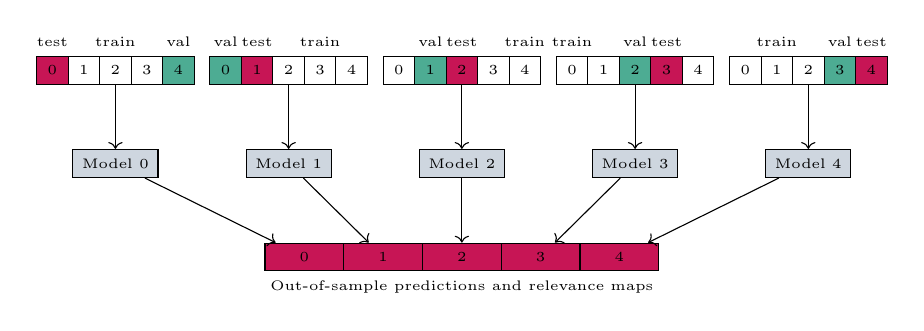
\begin{tikzpicture}
			\newcommand{\width}{0.4}
			\newcommand{\boxwidth}{0.4cm}
			\newcommand{\gap}{\width * 5.5}
			
			\node[
				draw=black,
				minimum width=\boxwidth,
				fill=cb-red-purple,
				label=\tiny{test}
			] at (0*\gap + 0*\width,0) {\tiny{0}};
			\node[
				draw=black,
				minimum width=\boxwidth
			] at (0*\gap + 1*\width,0) {\tiny{1}};
			\node[
				draw=black,
				minimum width=\boxwidth,
				label=\tiny{train}
			] (fold0) at (0*\gap + 2*\width,0) {\tiny{2}};			
			\node[
				draw=black,
				minimum width=\boxwidth
			] at (0*\gap + 3*\width,0) {\tiny{3}};			
			\node[
				draw=black,
				minimum width=\boxwidth,
				fill=cb-green,
				label=\tiny{val}
			] at (0*\gap + 4*\width,0) {\tiny{4}};
			
			\node[
				draw=black,
				minimum width=\boxwidth,
				fill=cb-green,
				label=\tiny{val}
			] at (1*\gap + 0*\width,0) {\tiny{0}};
			\node[
				draw=black,
				minimum width=\boxwidth,
				fill=cb-red-purple,
				label=\tiny{test}
			] at (1*\gap + 1*\width,0) {\tiny{1}};
			\node[
				draw=black,
				minimum width=\boxwidth
			] (fold1) at (1*\gap + 2*\width,0) {\tiny{2}};			
			\node[
				draw=black,
				minimum width=\boxwidth,
				label=\tiny{train}
			] at (1*\gap + 3*\width,0) {\tiny{3}};			
			\node[
				draw=black,
				minimum width=\boxwidth
			] at (1*\gap + 4*\width,0) {\tiny{4}};
			
			\node[
				draw=black,
				minimum width=\boxwidth
			] at (2*\gap + 0*\width,0) {\tiny{0}};
			\node[
				draw=black,
				minimum width=\boxwidth,
				fill=cb-green,
				label=\tiny{val}
			] at (2*\gap + 1*\width,0) {\tiny{1}};
			\node[
				draw=black,
				minimum width=\boxwidth,
				fill=cb-red-purple,
				label=\tiny{test}
			] (fold2) at (2*\gap + 2*\width,0) {\tiny{2}};			
			\node[
				draw=black,
				minimum width=\boxwidth
			] at (2*\gap + 3*\width,0) {\tiny{3}};			
			\node[
				draw=black,
				minimum width=\boxwidth,
				label=\tiny{train}
			] at (2*\gap + 4*\width,0) {\tiny{4}};
			
			\node[
				draw=black,
				minimum width=\boxwidth,
				label=\tiny{train}
			] at (3*\gap + 0*\width,0) {\tiny{0}};
			\node[
				draw=black,
				minimum width=\boxwidth
			] at (3*\gap + 1*\width,0) {\tiny{1}};
			\node[
				draw=black,
				minimum width=\boxwidth,
				fill=cb-green,
				label=\tiny{val}
			] (fold3) at (3*\gap + 2*\width,0) {\tiny{2}};			
			\node[
				draw=black,
				minimum width=\boxwidth,
				fill=cb-red-purple,
				label=\tiny{test}
			] at (3*\gap + 3*\width,0) {\tiny{3}};			
			\node[
				draw=black,
				minimum width=\boxwidth
			] at (3*\gap + 4*\width,0) {\tiny{4}};

			\node[
				draw=black,
				minimum width=\boxwidth
			] at (4*\gap + 0*\width,0) {\tiny{0}};
			\node[
				draw=black,
				minimum width=\boxwidth,
				label=\tiny{train}
			] at (4*\gap + 1*\width,0) {\tiny{1}};
			\node[
				draw=black,
				minimum width=\boxwidth
			] (fold4) at (4*\gap + 2*\width,0) {\tiny{2}};			
			\node[
				draw=black,
				minimum width=\boxwidth,
				fill=cb-green,
				label=\tiny{val}
			] at (4*\gap + 3*\width,0) {\tiny{3}};			
			\node[
				draw=black,
				minimum width=\boxwidth,
				fill=cb-red-purple,
				label=\tiny{test}
			] at (4*\gap + 4*\width,0) {\tiny{4}};
			
			\node[draw=black, fill=cb-gray!25] (model0) at ($ (fold0.south) - (0, 1) $) {\tiny{Model 0}};
			\node[draw=black, fill=cb-gray!25] (model1) at ($ (fold1.south) - (0, 1) $) {\tiny{Model 1}};
			\node[draw=black, fill=cb-gray!25] (model2) at ($ (fold2.south) - (0, 1) $) {\tiny{Model 2}};
			\node[draw=black, fill=cb-gray!25] (model3) at ($ (fold3.south) - (0, 1) $) {\tiny{Model 3}};
			\node[draw=black, fill=cb-gray!25] (model4) at ($ (fold4.south) - (0, 1) $) {\tiny{Model 4}};
			
			\node[draw=black, fill=cb-red-purple, minimum width=1cm, label=below:{\tiny{Out-of-sample predictions and relevance maps}}] (pred2) at ($ (model2.south) - (0, 1) $) {\tiny{2}};
			\node[draw=black, fill=cb-red-purple, minimum width=1cm] (pred1) at ($ (model2.south) - (1, 1) $) {\tiny{1}};
			\node[draw=black, fill=cb-red-purple, minimum width=1cm] (pred0) at ($ (model2.south) - (2, 1) $) {\tiny{0}};
			\node[draw=black, fill=cb-red-purple, minimum width=1cm] (pred3) at ($ (model2.south) - (-1, 1) $) {\tiny{3}};
			\node[draw=black, fill=cb-red-purple, minimum width=1cm] (pred4) at ($ (model2.south) - (-2, 1) $) {\tiny{4}};
			
			\draw[->] (fold0) -- (model0);
			\draw[->] (fold1) -- (model1);
			\draw[->] (fold2) -- (model2);
			\draw[->] (fold3) -- (model3);
			\draw[->] (fold4) -- (model4);
			
			\draw[->] (model0) -- (pred0);
			\draw[->] (model1) -- (pred1);
			\draw[->] (model2) -- (pred2);
			\draw[->] (model3) -- (pred3);
			\draw[->] (model4) -- (pred4);			
		\end{tikzpicture}
	\end{frame}	
	
	\begin{frame}{Dementia: Modelling} % Hyperparameter results
		\pgfplotsset{
			only if/.style args={entry of ####1 is ####2}{
				/pgfplots/boxplot/data filter/.code={
					\edef\tempa{\thisrow{####1}}
					\edef\tempb{####2}
					\ifx\tempa\tempb
					\else
						\def\pgfmathresult{}
					\fi
				}
			}
		}
		
		\centering
		\begin{tikzpicture}
			\begin{groupplot}[
  			    group style={
  				    group size=2 by 6,
  				    horizontal sep=0.25cm,
  				    vertical sep=0.6cm,
  			    },
  			    height=0.22\textwidth,
  			    width=0.37\textwidth,
				boxplot,
				boxplot/draw direction=y,
				boxplot/box extend=0.4,
				xtick style={draw=none},
				every x tick label/.append style={font=\tiny, text height=0.225em},
				every y tick label/.append style={font=\tiny}
			]
			
				\nextgroupplot[
					table/y=val_loss,
					ymin=0.38,
					ymax=0.82,
					xtick={1, 2, 3, 4, 5},
					xticklabels={0, 1, 2, 3, 4},
					ytick={0.4, 0.5, 0.6, 0.7, 0.8},
					ytick pos=left,
					ymajorgrids=true,
					ymajorticks=true,
					box plot width/.initial=2em,
					ylabel=\tiny{Loss},
				]
					\addplot[
						fill=cb-green,
						draw=black
					] table [
						col sep=comma,
						only if={entry of fold is 0}
					] {data/dementia_hyperparameters/summary.csv};
					\addplot[
						fill=cb-orange,
						draw=black
					] table [
						col sep=comma,
						only if={entry of fold is 1}
					] {data/dementia_hyperparameters/summary.csv};
					\addplot[
						fill=cb-blue,
						draw=black
					] table [
						col sep=comma,
						only if={entry of fold is 2}
					] {data/dementia_hyperparameters/summary.csv};
					\addplot[
						fill=cb-red-purple,
						draw=black
					] table [
						col sep=comma,
						only if={entry of fold is 3}
					] {data/dementia_hyperparameters/summary.csv};
					\addplot[
						fill=cb-pink,
						draw=black
					] table [
						col sep=comma,
						only if={entry of fold is 4}
					] {data/dementia_hyperparameters/summary.csv};

				\nextgroupplot[
					table/y=val_accuracy,
					xticklabels={,,},
					ymin=0.75,
					ymax=0.9,
					ytick={0.75, 0.8, 0.85, 0.9},
					yticklabels={{75\%}, {80\%}, {85\%}, {90\%}},
					ytick pos=right,
					ymajorgrids=true,
					ymajorticks=true,
					ylabel=\tiny{Accuracy}
				]
					\addplot[
						fill=cb-green,
						draw=black
					] table [
						col sep=comma,
						only if={entry of fold is 0}
					] {data/dementia_hyperparameters/summary.csv};
					\addplot[
						fill=cb-orange,
						draw=black
					] table [
						col sep=comma,
						only if={entry of fold is 1}
					] {data/dementia_hyperparameters/summary.csv};
					\addplot[
						fill=cb-blue,
						draw=black
					] table [
						col sep=comma,
						only if={entry of fold is 2}
					] {data/dementia_hyperparameters/summary.csv};
					\addplot[
						fill=cb-red-purple,
						draw=black
					] table [
						col sep=comma,
						only if={entry of fold is 3}
					] {data/dementia_hyperparameters/summary.csv};
					\addplot[
						fill=cb-pink,
						draw=black
					] table [
						col sep=comma,
						only if={entry of fold is 4}
					] {data/dementia_hyperparameters/summary.csv};

				\nextgroupplot[
					table/y=val_loss,
					xtick={1, 2},
					ymin=0.38,
					ymax=0.82,
					xticklabels={true, false},
					ymajorgrids=true,
					yticklabels={,,},
					ymajorticks=false
				]
					\addplot[
						fill=cb-green,
						draw=black
					] table [
						col sep=comma,
						only if={entry of pretrained is True}
					] {data/dementia_hyperparameters/summary.csv};
					\addplot[
						fill=cb-orange,
						draw=black
					] table [
						col sep=comma,
						only if={entry of pretrained is False}
					] {data/dementia_hyperparameters/summary.csv};
					
				\nextgroupplot[
					table/y=val_accuracy,
					ymin=0.75,
					ymax=0.9,
					xticklabels={,,},
					ymajorgrids=true,
					yticklabels={,,},
					ymajorticks=false
				]
					\addplot[
						fill=cb-green,
						draw=black
					] table [
						col sep=comma,
						only if={entry of pretrained is True}
					] {data/dementia_hyperparameters/summary.csv};
					\addplot[
						fill=cb-orange,
						draw=black
					] table [
						col sep=comma,
						only if={entry of pretrained is False}
					] {data/dementia_hyperparameters/summary.csv};
					
				\nextgroupplot[
					table/y=val_loss,
					xtick={1, 2, 3},
					ymin=0.38,
					ymax=0.82,
					xticklabels={stepwise, cycle, cyclical},
					ymajorgrids=true,
					yticklabels={,,},
					ymajorticks=false
				]
					\addplot[
						fill=cb-green,
						draw=black
					] table [
						col sep=comma,
						only if={entry of learning_rate is stepwise}
					] {data/dementia_hyperparameters/summary.csv};
					\addplot[
						fill=cb-orange,
						draw=black
					] table [
						col sep=comma,
						only if={entry of learning_rate is cycle}
					] {data/dementia_hyperparameters/summary.csv};
					\addplot[
						fill=cb-blue,
						draw=black
					] table [
						col sep=comma,
						only if={entry of learning_rate is cyclical}
					] {data/dementia_hyperparameters/summary.csv};
					
				\nextgroupplot[
					table/y=val_accuracy,
					ymin=0.75,
					ymax=0.9,
					xticklabels={,,},
					ymajorgrids=true,
					yticklabels={,,},
					ymajorticks=false
				]
					\addplot[
						fill=cb-green,
						draw=black
					] table [
						col sep=comma,
						only if={entry of learning_rate is stepwise}
					] {data/dementia_hyperparameters/summary.csv};
					\addplot[
						fill=cb-orange,
						draw=black
					] table [
						col sep=comma,
						only if={entry of learning_rate is cycle}
					] {data/dementia_hyperparameters/summary.csv};
					\addplot[
						fill=cb-blue,
						draw=black
					] table [
						col sep=comma,
						only if={entry of learning_rate is cyclical}
					] {data/dementia_hyperparameters/summary.csv};
					
				\nextgroupplot[
					table/y=val_loss,
					xtick={1, 2},
					ymin=0.38,
					ymax=0.82,
					xticklabels={light, heavy},
					ymajorgrids=true,
					yticklabels={,,},
					ymajorticks=false
				]
					\addplot[
						fill=cb-green,
						draw=black
					] table [
						col sep=comma,
						only if={entry of augmenter is baseline}
					] {data/dementia_hyperparameters/summary.csv};
					\addplot[
						fill=cb-orange,
						draw=black
					] table [
						col sep=comma,
						only if={entry of augmenter is heavy}
					] {data/dementia_hyperparameters/summary.csv};
					
				\nextgroupplot[
					table/y=val_accuracy,
					ymin=0.75,
					ymax=0.9,
					xticklabels={,,},
					ymajorgrids=true,
					yticklabels={,,},
					ymajorticks=false
				]
					\addplot[
						fill=cb-green,
						draw=black
					] table [
						col sep=comma,
						only if={entry of augmenter is baseline}
					] {data/dementia_hyperparameters/summary.csv};
					\addplot[
						fill=cb-orange,
						draw=black
					] table [
						col sep=comma,
						only if={entry of augmenter is heavy}
					] {data/dementia_hyperparameters/summary.csv};
					
				\nextgroupplot[
					table/y=val_loss,
					xtick={1, 2},
					ymin=0.38,
					ymax=0.82,
					xticklabels={0.25, 0.50},
					ymajorgrids=true,
					yticklabels={,,},
					ymajorticks=false
				]
					\addplot[
						fill=cb-green,
						draw=black
					] table [
						col sep=comma,
						only if={entry of dropout is 0.25}
					] {data/dementia_hyperparameters/summary.csv};
					\addplot[
						fill=cb-orange,
						draw=black
					] table [
						col sep=comma,
						only if={entry of dropout is 0.5}
					] {data/dementia_hyperparameters/summary.csv};

				\nextgroupplot[
					table/y=val_accuracy,
					ymin=0.75,
					ymax=0.9,
					xticklabels={,,},
					ymajorgrids=true,
					yticklabels={,,},
					ymajorticks=false
				]
					\addplot[
						fill=cb-green,
						draw=black
					] table [
						col sep=comma,
						only if={entry of dropout is 0.25}
					] {data/dementia_hyperparameters/summary.csv};
					\addplot[
						fill=cb-orange,
						draw=black
					] table [
						col sep=comma,
						only if={entry of dropout is 0.5}
					] {data/dementia_hyperparameters/summary.csv};
					
				\nextgroupplot[
					table/y=val_loss,
					xtick={1, 2},
					ymin=0.38,
					ymax=0.82,
					xticklabels={$10^{-2}$, $10^{-3}$},
					ymajorgrids=true,
					yticklabels={,,},
					ymajorticks=false
				]
					\addplot[
						fill=cb-green,
						draw=black
					] table [
						col sep=comma,
						only if={entry of weight_decay is 0.01}
					] {data/dementia_hyperparameters/summary.csv};
					\addplot[
						fill=cb-orange,
						draw=black
					] table [
						col sep=comma,
						only if={entry of weight_decay is 0.001}
					] {data/dementia_hyperparameters/summary.csv};
		
				\nextgroupplot[
					table/y=val_accuracy,
					ymin=0.75,
					ymax=0.9,
					xticklabels={,,},
					ymajorgrids=true,
					yticklabels={,,},
					ymajorticks=false
				]
					\addplot[
						fill=cb-green,
						draw=black
					] table [
						col sep=comma,
						only if={entry of weight_decay is 0.01}
					] {data/dementia_hyperparameters/summary.csv};
					\addplot[
						fill=cb-orange,
						draw=black
					] table [
						col sep=comma,
						only if={entry of weight_decay is 0.001}
					] {data/dementia_hyperparameters/summary.csv};
					
			\end{groupplot}
			\node[anchor=south, inner sep=0pt, text depth=0] at ($ (group c1r1.north)!0.5!(group c2r1.north) + (0,0.07) $) {\tiny{\textbf{Fold}}};
			\node[anchor=south, inner sep=0pt, text depth=0] at ($ (group c1r2.north)!0.5!(group c2r2.north) + (0,0.07) $) {\tiny{\textbf{Pretrained}}};
			\node[anchor=south, inner sep=0pt, text depth=0] at ($ (group c1r3.north)!0.5!(group c2r3.north) + (0,0.07) $) {\tiny{\textbf{Learning rate schedule}}};
			\node[anchor=south, inner sep=0pt, text depth=0] at ($ (group c1r4.north)!0.5!(group c2r4.north) + (0,0.07) $) {\tiny{\textbf{Augmenter}}};
			\node[anchor=south, inner sep=0pt, text depth=0] at ($ (group c1r5.north)!0.5!(group c2r5.north) + (0,0.07) $) {\tiny{\textbf{Dropout}}};
			\node[anchor=south, inner sep=0pt, text depth=0] at ($ (group c1r6.north)!0.5!(group c2r6.north) + (0,0.07) $) {\tiny{\textbf{Weight decay}}};
			
		\end{tikzpicture}
	\end{frame}
	
	\begin{frame}{Dementia: Predictive performance} % Overall
		\centering
		\pgfplotstableread[col sep=comma]{data/dementia_predictions/dementia_test_distributions.csv}\dementiadistributions
		\pgfplotstableread[col sep=comma]{data/dementia_predictions/dementia_test_predictions.csv}\dementiapredictions
		\pgfplotstableread[col sep=comma]{data/dementia_predictions/dementia_test_auc.csv}\dementiaauc
		
        \newcommand{\ymin}{-0.35}
        \newcommand{\ymax}{1.05}
        \begin{tikzpicture}
            \begin{axis}[
                name=distributions,
                height=0.4\textwidth,
                width=\textwidth,
                xtick pos=bottom,
                ymajorticks=false,
                xmin=0,
                xmax=1,
                ymin=\ymin,
                ymax=\ymax,
                xlabel=\scriptsize{Prediction},
                every tick label/.append style={font=\scriptsize}
            ]
                \addplot[name path=controls, draw=controls-default, very thick] table [x=prediction,y=controls]{\dementiadistributions};
                \addplot[name path=cases, draw=cases-default, very thick] table [x=prediction,y=cases]{\dementiadistributions};
                \addplot[name path=zero, draw=black] coordinates {(0,0) (1,0)};
                \addplot[fill=controls-default, opacity=0.2] fill between [of=zero and controls];
                \addplot[fill=cases-default, opacity=0.2] fill between [of=zero and cases];
                \addplot[
                    scatter/classes={
                        control={controls-default, draw=black, opacity=0.5}, 
                        case={cases-default, draw=black, opacity=0.5}
                    },
                    scatter, 
                    mark=*, 
                    only marks,
                    point meta=explicit symbolic
                ] table [
                    y expr=\thisrow{y} * -0.15 - 0.1, 
                    meta=class, 
                    each nth point=\N
                ] {\dementiapredictions};
                \addplot[dashed] coordinates {(0.5, \ymin) (0.5, \ymax)};
            \end{axis}
            \node[anchor=south west] at ($ (distributions.south east) + (0,0.28) $) {\tiny{Controls}};
            \node[anchor=south west] at ($ (distributions.south east) + (0,0.0) $) {\tiny{Cases}};
            \node[anchor=south,align=center] at (distributions.north) {\tiny{$t$}};
        \end{tikzpicture}
        
        \colorlet{roc-curve}{cb-blue-purple}
        \newcommand{\length}{0.8\textwidth}
        \newcommand{\tx}{0.130}
        \newcommand{\ty}{0.809}
        \begin{figure}
        \begin{subfigure}{0.49\textwidth}
        \centering
        \begin{tikzpicture}
            \begin{axis}[
                height=\length,
                width=\length,
                xtick pos=bottom,
                ytick pos=left,
                xtick={0.5, 1, \tx},
                ytick={0.5, 1, \ty},
                xmin=-0,
                xmax=1,
                ymin=0,
                ymax=1,
                xlabel=\scriptsize{FPR},
                ylabel=\scriptsize{TPR},
                every tick label/.append style={font=\scriptsize}
            ]
                \addplot[dotted] coordinates {(\tx, 0) (\tx, 1)};
                \addplot[dotted] coordinates {(0, \ty) (1, \ty)};
                \addplot[draw=roc-curve,very thick] table [x=fpr,y=tpr] {\dementiaauc};
                \addplot[] coordinates {(0,0) (1,1)};
                \node[anchor=south east, inner sep=5pt] at (axis cs: 1, 0) {\textbf{\scriptsize{AUC 0.899}}};
                \node[
                    name=threshold,
                    draw=black, 
                    fill=roc-curve,
                    star,
                    star points=5,
                    inner sep=0cm,
                    minimum height=0.1cm,
                    minimum width=0.2cm
                ] at (axis cs: \tx, \ty) {};
                \node[anchor=north west] at (threshold.east) {\tiny{$t=0.5$}};
            \end{axis}
        \end{tikzpicture}
        \end{subfigure}
        \begin{subfigure}{0.49\textwidth}
        \centering
        \begin{tabular}{c|c|c|c|}
            \multicolumn{2}{c}{} & \multicolumn{2}{c}{\scriptsize{Predicted}} \\
            \cline{3-4}
            \multicolumn{1}{l}{\parbox[t]{2mm}{\multirow{4}{*}{\rotatebox[origin=c]{90}{\scriptsize{Observed}}}}} & \multicolumn{1}{c|}{} & \scriptsize{\textbf{0}} & \scriptsize{\textbf{1}} \\
            \cline{2-4}
            &\scriptsize{\textbf{0}}&\scriptsize{626}&\scriptsize{94}\\
            \cline{2-4}
            &\scriptsize{\textbf{1}}&\scriptsize{138}&\scriptsize{582}\\
            \cline{2-4}
        \end{tabular}\\
        \vspace{0.3cm}
        \scriptsize{\textbf{Accuracy: 83.88\%}}
        \end{subfigure}
      	\end{figure}
	\end{frame}
	
	\begin{frame}{Dementia: Predictive performance} % Groups
		\centering
		\vfill
		\begin{tabular}{|c|c|c|c|}
			\hline
			\textbf{Site}&\textbf{Size}&\textbf{AUC}&\textbf{Accuracy}\\
			\hline
			\textcolor{red}{OASIS3 3.0T}&\textcolor{red}{430}&\textcolor{red}{0.841}&\textcolor{red}{76.9}\\
			\hline
			ADNI 1.5T&300&0.915&87.0\\
			\hline
			ADNI 3.0T&266&0.951&88.3\\
			\hline
			Oslo GE750&210&0.915&82.8\\
			\hline
			AIBL Site 1&90&0.920&87.7\\
			\hline
			ANM GE&72&0.853&81.9\\
			\hline
			MIRIAD&32&1.00&100\\
			\hline
			AIBL Site 2&22&0.892&86.3\\
			\hline
			ANM Picker&10&0.840&80.0\\
			\hline
			\textcolor{red}{OASIS3 1.5T}&\textcolor{red}{8}&\textcolor{red}{0.812}&\textcolor{red}{75.0}\\
			\hline
		\end{tabular}
		\vfill
	\end{frame}	
	
	\begin{frame}{Dementia: Relevance maps} % LRP Strategy
		\renewcommand{\arraystretch}{0.8}
		\centering
		\vfill
		\begin{tabular}{|c|c|}
	        \hline
	        \tiny{\textbf{Layer}}&\tiny{\textbf{LRP Strategy}}\\
	        \hline
	        \tiny{Input}&\tiny{-}\\
	        \hline
	        \tiny{Conv3D}&\tiny{\{flat: True\}}\\
	        \hline
	        \tiny{MaxPooling3D}&\tiny{-}\\
	        \hline
	        \tiny{Conv3D}&\tiny{\{flat: True\}}\\
	        \hline
	        \tiny{MaxPooling3D}&\tiny{-}\\
	        \hline
	        \tiny{Conv3D}&\tiny{\{$\alpha$: 1, $\beta$: 0\}}\\
	        \hline
	        \tiny{MaxPooling3D}&\tiny{-}\\
	        \hline
	        \tiny{Conv3D}&\tiny{\{$\alpha$: 1, $\beta$: 0\}}\\
	        \hline
	        \tiny{MaxPooling3D}&\tiny{-}\\
	        \hline
	        \tiny{Conv3D}&\tiny{\{$\alpha$: 1, $\beta$: 0\}}\\
	        \hline
	        \tiny{MaxPooling3D}&\tiny{-}\\
	        \hline
	        \tiny{Conv3D}&\tiny{\{$\alpha$: 1, $\beta$: 0\}}\\
	        \hline
	        \tiny{GlobalAveragePooling3D}&\tiny{-}\\
	        \hline
	        \tiny{Dropout}&\tiny{-}\\
	        \hline
	        \tiny{Dense}&\tiny{\{$\epsilon$: 0.25\}}\\
	        \hline
	    \end{tabular}
	    \vfill
	\end{frame}
	
	\begin{frame}{Dementia: Relevance maps} % Examples
		\vfill
		\centering
		\newcommand{\width}{3.5cm}
		\includegraphics[width=\width]{data/1398_1.png}
		\includegraphics[width=\width]{data/1504_1.png}
		\includegraphics[width=\width]{data/94405.png}
		\vfill
	\end{frame}

	\begin{frame}{Dementia: Relevance maps} % Summaries
		\centering
		\begin{tikzpicture}
			\node[] at (0,0) {\includegraphics[width=6cm]{data/dementia_summaries/test_average.png}};
		\end{tikzpicture}
	\end{frame}

	\begin{frame}{Dementia: Relevance maps} % Validation maps
		\centering
		\begin{tikzpicture}
			\node[label=below:{\tiny{Dementia model}}] at (0,0) {\includegraphics[width=2.75cm]{data/dementia_summaries/test_average.png}};
			\node[label=below:{\tiny{Dementia model with randomized images}}] at (4,0) {\includegraphics[width=2.75cm]{data/dementia_summaries/randomized_images_average.png}};
			\node[label=below:{\tiny{Sex model}}] at (0,-4) {\includegraphics[width=2.75cm]{data/dementia_summaries/sex_average.png}};
			\node[label=below:{\tiny{Model with randomized weights}}] at (4,-4) {\includegraphics[width=2.75cm]{data/dementia_summaries/randomized_weights_average.png}};
		\end{tikzpicture}
	\end{frame}

	{
    	\setbeamertemplate{footline}{\hspace{0.22cm} \hfill \textcolor{gray}{\tiny{\href{https://neuroquery.org/}{https://neuroquery.org/}}} \hfill \scriptsize{53} \hspace{0.24cm}\vspace{0.4cm}}
		\begin{frame}{Dementia: Relevance maps} % Neuroquery
			\vfill
			\centering
			\begin{tikzpicture}
				\node[label=below:Neuroquery] at (0, 0) {\includegraphics[width=5cm]{data/dementia_summaries/neuroquery.png}};
			\end{tikzpicture}
			\vfill
		\end{frame}
	}

	\begin{frame}{Dementia: Relevance maps} % Overlap 60th percentile
		\vfill
		\centering
		\begin{tikzpicture}
			\node[minimum width=4cm, minimum height=6.1cm, fill=black] (background) at (3.5, -2.05) {};
			\node[] at (2.5, 0) {
				\includegraphics[width=1cm, height=1cm]{data/dementia_overlap/dementia_overlap_test_60_saggital.png}
			};
			\node[] (dementia) at (3.5, 0) {
				\includegraphics[width=1cm, height=1cm]{data/dementia_overlap/dementia_overlap_test_60_coronal.png}
			};
			\node[] at (4.5, 0) {
				\includegraphics[width=1cm, height=1cm]{data/dementia_overlap/dementia_overlap_test_60_axial.png}
			};
			\node[] at (dementia.south) {\textcolor{white}{\tiny{dementia}}};
			
			
			\node[] at (2.5, -1.3) {
				\includegraphics[width=1cm, height=1cm]{data/dementia_overlap/dementia_overlap_sex_60_saggital.png}
			};
			\node[] (sex) at (3.5, -1.3) {
				\includegraphics[width=1cm, height=1cm]{data/dementia_overlap/dementia_overlap_sex_60_coronal.png}
			};
			\node[] at (4.5, -1.3) {
				\includegraphics[width=1cm, height=1cm]{data/dementia_overlap/dementia_overlap_sex_60_axial.png}
			};
			\node[] at (sex.south) {\textcolor{white}{\tiny{sex}}};
			
			\node[] at (2.5, -2.6) {
				\includegraphics[width=1cm, height=1cm]{data/dementia_overlap/dementia_overlap_randomized_weights_60_saggital.png}
			};
			\node[] (weights) at (3.5, -2.6) {
				\includegraphics[width=1cm, height=1cm]{data/dementia_overlap/dementia_overlap_randomized_weights_60_coronal.png}
			};
			\node[] at (4.5, -2.6) {
				\includegraphics[width=1cm, height=1cm]{data/dementia_overlap/dementia_overlap_randomized_weights_60_axial.png}
			};
			\node[] at (weights.south) {\textcolor{white}{\tiny{randomized weights}}};
			
			\node[] at (2.5, -3.9) {
				\includegraphics[width=1cm, height=1cm]{data/dementia_overlap/dementia_overlap_randomized_images_60_saggital.png}
			};
			\node[] (images) at (3.5, -3.9) {
				\includegraphics[width=1cm, height=1cm]{data/dementia_overlap/dementia_overlap_randomized_images_60_coronal.png}
			};
			\node[] at (4.5, -3.9) {
				\includegraphics[width=1cm, height=1cm]{data/dementia_overlap/dementia_overlap_randomized_images_60_axial.png}
			};
			\node[] at (images.south) {\textcolor{white}{\tiny{randomized images}}};
			
			\node[anchor=south, inner sep=0pt, text depth=0] (nq-text) at ($(background.south) + (0, 0.1) $) {\textcolor{white}{\tiny{NeuroQuery}}};
			\node[fill=red, anchor=east, inner sep=2pt] (nq-symbol) at ($ (nq-text.west) + (-0.1, 0) $) {};
			\node[anchor=east, inner sep=0pt, text depth=0] (rm-text) at ($ (nq-symbol.west) + (-0.3, 0) $) {\tiny{\textcolor{white}{LRP}}};
			\node[fill=green, anchor=east, inner sep=2pt] at ($ (rm-text.west) + (-0.1, 0) $) {};
			\node[fill=yellow, anchor=west, inner sep=2pt] (both-symbol) at ($ (nq-text.east) + (0.3, 0) $) {};
			\node[anchor=west, inner sep=0pt] at ($ (both-symbol.east) + (0.1, 0) $) {\textcolor{white}{\tiny{Overlap}}};
			
			\node[anchor=north] at (background.north) {\textcolor{white}{\scriptsize{60th percentile}}};
		\end{tikzpicture}
		\vfill
	\end{frame}	
	
	\begin{frame}{Dementia: Relevance maps} % Overlap 60th percentile
		\vfill
		\centering
		\begin{tikzpicture}
			\node[minimum width=4cm, minimum height=6.1cm, fill=black] (background) at (3.5, -2.05) {};
			\node[] at (2.5, 0) {
				\includegraphics[width=1cm, height=1cm]{data/dementia_overlap/dementia_overlap_test_60_saggital.png}
			};
			\node[] (dementia) at (3.5, 0) {
				\includegraphics[width=1cm, height=1cm]{data/dementia_overlap/dementia_overlap_test_60_coronal.png}
			};
			\node[] at (4.5, 0) {
				\includegraphics[width=1cm, height=1cm]{data/dementia_overlap/dementia_overlap_test_60_axial.png}
			};
			\node[] at (dementia.south) {\textcolor{white}{\tiny{dementia}}};
			
			
			\node[] at (2.5, -1.3) {
				\includegraphics[width=1cm, height=1cm]{data/dementia_overlap/dementia_overlap_sex_60_saggital.png}
			};
			\node[] (sex) at (3.5, -1.3) {
				\includegraphics[width=1cm, height=1cm]{data/dementia_overlap/dementia_overlap_sex_60_coronal.png}
			};
			\node[] at (4.5, -1.3) {
				\includegraphics[width=1cm, height=1cm]{data/dementia_overlap/dementia_overlap_sex_60_axial.png}
			};
			\node[] at (sex.south) {\textcolor{white}{\tiny{sex}}};
			
			\node[] at (2.5, -2.6) {
				\includegraphics[width=1cm, height=1cm]{data/dementia_overlap/dementia_overlap_randomized_weights_60_saggital.png}
			};
			\node[] (weights) at (3.5, -2.6) {
				\includegraphics[width=1cm, height=1cm]{data/dementia_overlap/dementia_overlap_randomized_weights_60_coronal.png}
			};
			\node[] at (4.5, -2.6) {
				\includegraphics[width=1cm, height=1cm]{data/dementia_overlap/dementia_overlap_randomized_weights_60_axial.png}
			};
			\node[] at (weights.south) {\textcolor{white}{\tiny{randomized weights}}};
			
			\node[] at (2.5, -3.9) {
				\includegraphics[width=1cm, height=1cm]{data/dementia_overlap/dementia_overlap_randomized_images_60_saggital.png}
			};
			\node[] (images) at (3.5, -3.9) {
				\includegraphics[width=1cm, height=1cm]{data/dementia_overlap/dementia_overlap_randomized_images_60_coronal.png}
			};
			\node[] at (4.5, -3.9) {
				\includegraphics[width=1cm, height=1cm]{data/dementia_overlap/dementia_overlap_randomized_images_60_axial.png}
			};
			\node[] at (images.south) {\textcolor{white}{\tiny{randomized images}}};
			
			\node[anchor=south, inner sep=0pt, text depth=0] (nq-text) at ($(background.south) + (0, 0.1) $) {\textcolor{white}{\tiny{NeuroQuery}}};
			\node[fill=red, anchor=east, inner sep=2pt] (nq-symbol) at ($ (nq-text.west) + (-0.1, 0) $) {};
			\node[anchor=east, inner sep=0pt, text depth=0] (rm-text) at ($ (nq-symbol.west) + (-0.3, 0) $) {\tiny{\textcolor{white}{LRP}}};
			\node[fill=green, anchor=east, inner sep=2pt] at ($ (rm-text.west) + (-0.1, 0) $) {};
			\node[fill=yellow, anchor=west, inner sep=2pt] (both-symbol) at ($ (nq-text.east) + (0.3, 0) $) {};
			\node[anchor=west, inner sep=0pt] at ($ (both-symbol.east) + (0.1, 0) $) {\textcolor{white}{\tiny{Overlap}}};
			
			\node[anchor=north] at (background.north) {\textcolor{white}{\scriptsize{60th percentile}}};
			
			\node[minimum width=3.5cm, minimum height=6.1cm, fill=black] (background) at (-0.15, -2.05) {};
			\node[inner sep=0pt] at (-1.25, 0) {
				\includegraphics[width=1cm, height=1cm]{data/dementia_overlap/dementia_overlap_test_30_saggital.png}
			};
			\node[inner sep=0pt] (dementia) at (-0.25, 0) {
				\includegraphics[width=1cm, height=1cm]{data/dementia_overlap/dementia_overlap_test_30_coronal.png}
			};
			\node[inner sep=0pt] at (0.75, 0) {
				\includegraphics[width=1cm, height=1cm]{data/dementia_overlap/dementia_overlap_test_30_axial.png}
			};
			
			
			\node[] at (-1.15, -1.3) {
				\includegraphics[width=1cm, height=1cm]{data/dementia_overlap/dementia_overlap_sex_30_saggital.png}
			};
			\node[] (sex) at (-0.15, -1.3) {
				\includegraphics[width=1cm, height=1cm]{data/dementia_overlap/dementia_overlap_sex_30_coronal.png}
			};
			\node[] at (0.85, -1.3) {
				\includegraphics[width=1cm, height=1cm]{data/dementia_overlap/dementia_overlap_sex_30_axial.png}
			};
			
			\node[] at (-1.15, -2.6) {
				\includegraphics[width=1cm, height=1cm]{data/dementia_overlap/dementia_overlap_randomized_weights_30_saggital.png}
			};
			\node[] (weights) at (-0.15, -2.6) {
				\includegraphics[width=1cm, height=1cm]{data/dementia_overlap/dementia_overlap_randomized_weights_30_coronal.png}
			};
			\node[] at (0.85, -2.6) {
				\includegraphics[width=1cm, height=1cm]{data/dementia_overlap/dementia_overlap_randomized_weights_30_axial.png}
			};
			
			\node[] at (-1.15, -3.9) {
				\includegraphics[width=1cm, height=1cm]{data/dementia_overlap/dementia_overlap_randomized_images_30_saggital.png}
			};
			\node[] (images) at (-0.15, -3.9) {
				\includegraphics[width=1cm, height=1cm]{data/dementia_overlap/dementia_overlap_randomized_images_30_coronal.png}
			};
			\node[] at (0.85, -3.9) {
				\includegraphics[width=1cm, height=1cm]{data/dementia_overlap/dementia_overlap_randomized_images_30_axial.png}
			};
			
			\node[anchor=north] at (background.north) {\textcolor{white}{\scriptsize{30th percentile}}};
			
			\node[minimum width=3.5cm, minimum height=6.1cm, fill=black] (background) at (7.15, -2.05) {};
			\node[inner sep=0pt] at (6.15, 0) {
				\includegraphics[width=1cm, height=1cm]{data/dementia_overlap/dementia_overlap_test_90_saggital.png}
			};
			\node[inner sep=0pt] (dementia) at (7.15, 0) {
				\includegraphics[width=1cm, height=1cm]{data/dementia_overlap/dementia_overlap_test_90_coronal.png}
			};
			\node[inner sep=0pt] at (8.15, 0) {
				\includegraphics[width=1cm, height=1cm]{data/dementia_overlap/dementia_overlap_test_90_axial.png}
			};
			
			
			\node[] at (6.15, -1.3) {
				\includegraphics[width=1cm, height=1cm]{data/dementia_overlap/dementia_overlap_sex_90_saggital.png}
			};
			\node[] (sex) at (7.15, -1.3) {
				\includegraphics[width=1cm, height=1cm]{data/dementia_overlap/dementia_overlap_sex_90_coronal.png}
			};
			\node[] at (8.15, -1.3) {
				\includegraphics[width=1cm, height=1cm]{data/dementia_overlap/dementia_overlap_sex_90_axial.png}
			};
			
			\node[] at (6.15, -2.6) {
				\includegraphics[width=1cm, height=1cm]{data/dementia_overlap/dementia_overlap_randomized_weights_90_saggital.png}
			};
			\node[] (weights) at (7.15, -2.6) {
				\includegraphics[width=1cm, height=1cm]{data/dementia_overlap/dementia_overlap_randomized_weights_90_coronal.png}
			};
			\node[] at (8.15, -2.6) {
				\includegraphics[width=1cm, height=1cm]{data/dementia_overlap/dementia_overlap_randomized_weights_90_axial.png}
			};
			
			\node[] at (6.15, -3.9) {
				\includegraphics[width=1cm, height=1cm]{data/dementia_overlap/dementia_overlap_randomized_images_90_saggital.png}
			};
			\node[] (images) at (7.15, -3.9) {
				\includegraphics[width=1cm, height=1cm]{data/dementia_overlap/dementia_overlap_randomized_images_90_coronal.png}
			};
			\node[] at (8.15, -3.9) {
				\includegraphics[width=1cm, height=1cm]{data/dementia_overlap/dementia_overlap_randomized_images_90_axial.png}
			};
			
			\node[anchor=north] at (background.north) {\textcolor{white}{\scriptsize{90th percentile}}};
		\end{tikzpicture}
		\vfill
	\end{frame}	

	\begin{frame}{Dementia: Relevance maps} % Dice coefficient
		\vfill
		\centering
		\begin{tikzpicture}
			\begin{axis}[
				height=0.6\textwidth,
				width=0.6\textwidth,
				xmin=0,
				xmax=1,
				tick label style={font=\footnotesize},
				xtick={0, 0.2, 0.4, 0.6, 0.8, 1},
				xticklabels={0, 20, 40, 60, 80, 100},
				xlabel=\footnotesize{Percentile},
				ylabel=\footnotesize{Dice coefficient},
				xtick style={draw=none},
				ytick style={draw=none},
				xmajorgrids=true,
				ymajorgrids=true
			]
				\addplot[very thick,draw=cb-blue-purple] table [col sep=comma, x=thresholds, y=test] {data/overlap_measures/dementia_dice.csv};\label{trace:dementia}
				\addplot[very thick,draw=cb-green] table [col sep=comma, x=thresholds, y=sex] {data/overlap_measures/dementia_dice.csv};\label{trace:sex}
				\addplot[very thick,draw=cb-gray] table [col sep=comma, x=thresholds, y=randomized_weights] {data/overlap_measures/dementia_dice.csv};\label{trace:weights}
				\addplot[very thick,draw=cb-orange] table [col sep=comma, x=thresholds, y=randomized_images] {data/overlap_measures/dementia_dice.csv};\label{trace:images}
				
				\coordinate (legend) at (axis cs: 1.02,0.29);
			\end{axis}
			
			\newcommand*{\DrawLine}[2][]{%
    			\tikz [baseline] \draw [####1] (0,0.5ex) -- ++(####2,0);%
			}
			\node[font=\scriptsize, anchor=west, align=left ] at (legend) {\DrawLine[draw=cb-blue-purple, very thick]{0.4cm} Dementia\\ \DrawLine[draw=cb-green, very thick]{0.4cm} Sex\\ \DrawLine[draw=cb-gray, very thick]{0.4cm} Random weights\\ \DrawLine[draw=cb-orange, very thick]{0.4cm} Random images};
		\end{tikzpicture}
		\vfill
	\end{frame}
	
	\begin{frame}{Dementia: Relevance maps} % Other measures
		\centering
		\newcommand{\measuresubplot}[4]{
			\nextgroupplot[
				title=\scriptsize{####1},
				tick label style={font=\tiny},
				ytick={0, 0.2, 0.4, 0.6, 0.8, 1},
				xticklabels=####2,
				xtick={0, 0.2, 0.4, 0.6, 0.8, 1},
				yticklabels=####3,
				xlabel=####4,
				xtick style={draw=none},
				ytick style={draw=none},
				xmajorgrids=true,
				ymajorgrids=true
			]
				\addplot[very thick,draw=cb-blue-purple] table [col sep=comma, x=thresholds, y=test] {data/overlap_measures/dementia_####1.csv};\label{trace:dementia}
				\addplot[very thick,draw=cb-green] table [col sep=comma, x=thresholds, y=sex] {data/overlap_measures/dementia_####1.csv};\label{trace:sex}
				\addplot[very thick,draw=cb-gray] table [col sep=comma, x=thresholds, y=randomized_weights] {data/overlap_measures/dementia_####1.csv};\label{trace:weights}
				\addplot[very thick,draw=cb-orange] table [col sep=comma, x=thresholds, y=randomized_images] {data/overlap_measures/dementia_####1.csv};\label{trace:images}
		}
		\begin{tikzpicture}
			\begin{groupplot}[
  			    group style={
  				    group size=2 by 1,
  				    horizontal sep=0.1cm
  			    },
  			    height=0.45\textwidth,
  			    width=0.45\textwidth,
				xmin=0,
				xmax=1,
				ymin=0,
				ymax=1
			]
				\measuresubplot{recall}{{0, 20, 40, 60, 80, 100}}{{0, 0.2, 0.4, 0.6, 0.8, 1}}{\tiny{Percentile}}
				\measuresubplot{precision}{{,,}}{{,,}}{}
			\end{groupplot}
			
			\newcommand*{\DrawLine}[2][]{%
    			\tikz [baseline] \draw [####1] (0,0.5ex) -- ++(####2,0);%
			}
			\node[font=\scriptsize] at ($ (group c1r1.south)!0.5!(group c2r1.south) + (0, -1.3) $) {\DrawLine[draw=cb-blue-purple, very thick]{0.3cm} Dementia\hspace{0.2cm}\DrawLine[draw=cb-green, very thick]{0.3cm} Sex\hspace{0.2cm}\DrawLine[draw=cb-gray, very thick]{0.3cm} Randomized weights\hspace{0.2cm}\DrawLine[draw=cb-orange, very thick]{0.3cm} Randomized images};
		\end{tikzpicture}
	\end{frame}
	
	\begin{frame}{Dementia: Relevance maps} % Region-wise single
		\vfill
		\centering
		\begin{tikzpicture}
			\node[label=Mean activation per region,draw=black,inner sep=0pt] at (0, 0) (test) {\includegraphics[width=8cm]{data/dementia_regions/test.png}};
			\node[rotate=90, anchor=south] at (test.west) {\footnotesize{NeuroQuery}};
			\node[anchor=north] at (test.south) {\footnotesize{LRP}};
		\end{tikzpicture}
		\vfill
	\end{frame}
	
	\begin{frame}{Dementia: Relevance maps} % Region-wise comparison
		\vfill
		\centering
		\begin{tikzpicture}
			\newcommand{\width}{5cm}
			\node[draw=black,inner sep=0pt] at (0, 0) (test) {\includegraphics[width=\width]{data/dementia_regions/test.png}};
			\node[anchor=south, inner sep=3pt] at (test.north) {\footnotesize{Dementia}};
			
			\node[draw=black,inner sep=0pt] at (5.5, 0) (test) {\includegraphics[width=\width]{data/dementia_regions/sex.png}};
			\node[anchor=south, inner sep=3pt] at (test.north) {\footnotesize{Sex}};
			
			\node[draw=black,inner sep=0pt] at (0, -3) (test) {\includegraphics[width=\width]{data/dementia_regions/randomized_weights.png}};
			\node[anchor=south, inner sep=3pt] at (test.north) {\footnotesize{Randomized weights}};
			
			\node[draw=black,inner sep=0pt] at (5.5, -3) (test) {\includegraphics[width=\width]{data/dementia_regions/randomized_images.png}};
			\node[anchor=south, inner sep=3pt] at (test.north) {\footnotesize{Randomized images}};
		\end{tikzpicture}
		\vfill	
	
	\end{frame}

	\begin{frame}{Dementia: Relevance maps} % Masking start
		\begin{tikzpicture}
			\node[inner sep=0pt] (image0) at (0, 0) {
				\includegraphics[width=1.5cm]{data/dementia_masks/validation_image_0.png}
			};
			
			\node[] at ($ (image0.north) + (0, 2.2) $) {\footnotesize{Iteration 0}};
			
			\node[draw=black,fill=cb-blue-purple!20, inner sep=10pt] (model) at (4.5, -3.2) {\scriptsize{Dementia model}};
			
			\node[] at (9.7,-4.8) {};
		\end{tikzpicture}
	\end{frame}

	\begin{frame}{Dementia: Relevance maps} % Masking prediction 0
		\begin{tikzpicture}
			\node[inner sep=0pt] (image0) at (0, 0) {
				\includegraphics[width=1.5cm]{data/dementia_masks/validation_image_0.png}
			};
			
			\node[draw=black,fill=cb-blue-purple!20, inner sep=10pt] (model) at (4.5, -3.2) {\scriptsize{Dementia model}};
			
			\node[] at ($ (image0.north) + (0, 2.2) $) {\footnotesize{Iteration 0}};
			
			\node[] (pred0) at ($ (image0.south) - (0, 4) $) {\footnotesize{0.93}};
			\node[] at (9.7,-4.8) {};
			
			\draw[->,dashed] (image0.south) to [out=270,in=180] (model.west);
			\draw[->,dashed] (model.south) to [out=270,in=0] (pred0.east);
			
		\end{tikzpicture}
	\end{frame}

	\begin{frame}{Dementia: Relevance maps} % Masking heatmap 0
		\begin{tikzpicture}
			\node[inner sep=0pt] (image0) at (0, 0) {
				\includegraphics[width=1.5cm]{data/dementia_masks/validation_image_0.png}
			};
			
			\node[inner sep=0pt, label=\tiny{Validation}] (heatmap0) at (2.5, 1.5) {
				\includegraphics[width=1.5cm]{data/dementia_masks/validation_heatmap_0.png}
			};
			
			\node[draw=black,fill=cb-blue-purple!20, inner sep=10pt] (model) at (4.5, -3.2) {\scriptsize{Dementia model}};
			
			\node[] at ($ (image0.north) + (0, 2.2) $) {\footnotesize{Iteration 0}};
			
			\node[] at ($ (image0.south) - (0, 4) $) {\footnotesize{0.93}};
			\node[] at (9.7,-4.8) {};
			
			\draw[->] (image0.east) to [out=0, in=180] (heatmap0.west);
			
		\end{tikzpicture}
	\end{frame}

	\begin{frame}{Dementia: Relevance maps} % Masking image 1
		\begin{tikzpicture}
			\node[inner sep=0pt] (image0) at (0, 0) {
				\includegraphics[width=1.5cm]{data/dementia_masks/validation_image_0.png}
			};
			
			\node[inner sep=0pt, label=\tiny{Validation}] (heatmap0) at (2.5, 1.5) {
				\includegraphics[width=1.5cm]{data/dementia_masks/validation_heatmap_0.png}
			};
			\node[draw=black, fill=cb-gray!20] (mask0) at (2.5, 0) {\scriptsize{Masking}};
			\node[inner sep=0pt] (image1) at (2.5, -1.5) {
				\includegraphics[width=1.5cm]{data/dementia_masks/validation_image_1.png}
			};
			
			\node[draw=black,fill=cb-blue-purple!20, inner sep=10pt] (model) at (4.5, -3.2) {\scriptsize{Dementia model}};
			
			\node[] at ($ (image0.north) + (0, 2.2) $) {\footnotesize{Iteration 0}};
			
			\node[] at ($ (image0.south) - (0, 4) $) {\footnotesize{0.93}};
			\node[] at (9.7,-4.8) {};
			
			\draw[->] (image0.east) to [out=0, in=180] (heatmap0.west);
			\draw[->] (heatmap0.south) -- (mask0.north);
			\draw[->] (mask0.south) -- (image1.north);
			
		\end{tikzpicture}
	\end{frame}

	\begin{frame}{Dementia: Relevance maps} % Masking prediction 1
		\begin{tikzpicture}
			\node[inner sep=0pt] (image0) at (0, 0) {
				\includegraphics[width=1.5cm]{data/dementia_masks/validation_image_0.png}
			};
			
			\node[inner sep=0pt, label=\tiny{Validation}] (heatmap0) at (2.5, 1.5) {
				\includegraphics[width=1.5cm]{data/dementia_masks/validation_heatmap_0.png}
			};
			\node[draw=black, fill=cb-gray!20] (mask0) at (2.5, 0) {\scriptsize{Masking}};
			\node[inner sep=0pt] (image1) at (2.5, -1.5) {
				\includegraphics[width=1.5cm]{data/dementia_masks/validation_image_1.png}
			};
			
			\node[draw=black,fill=cb-blue-purple!20, inner sep=10pt] (model) at (4.5, -3.2) {\scriptsize{Dementia model}};
			
			\node[] at ($ (image0.north) + (0, 2.2) $) {\footnotesize{Iteration 0}};
			\node[] at ($ (heatmap0.north) + (0, 0.7) $) {\footnotesize{Iteration 1}};
			
			\node[] at ($ (image0.south) - (0, 4) $) {\footnotesize{0.93}};
			\node[] (pred1) at ($ (image1.south) - (0, 2.5) $) {\footnotesize{0.87}};
			\node[] at (9.7,-4.8) {};
			
			\draw[->] (image0.east) to [out=0, in=180] (heatmap0.west);
			\draw[->] (heatmap0.south) -- (mask0.north);
			\draw[->] (mask0.south) -- (image1.north);
			\draw[->,dashed] (image1.south) to [out=270,in=180] (model.west);
			\draw[->,dashed] (model.south) to [out=270,in=90] (pred1);
			
		\end{tikzpicture}
	\end{frame}

	\begin{frame}{Dementia: Relevance maps} % Masking heatmap 2
		\begin{tikzpicture}
			\node[inner sep=0pt] (image0) at (0, 0) {
				\includegraphics[width=1.5cm]{data/dementia_masks/validation_image_0.png}
			};
			
			\node[inner sep=0pt, label=\tiny{Validation}] (heatmap0) at (2.5, 1.5) {
				\includegraphics[width=1.5cm]{data/dementia_masks/validation_heatmap_0.png}
			};
			\node[draw=black, fill=cb-gray!20] (mask0) at (2.5, 0) {\scriptsize{Masking}};
			\node[inner sep=0pt] (image1) at (2.5, -1.5) {
				\includegraphics[width=1.5cm]{data/dementia_masks/validation_image_1.png}
			};
			
			\node[inner sep=0pt] (heatmap1) at (5, 1.5) {
				\includegraphics[width=1.5cm]{data/dementia_masks/validation_heatmap_1.png}
			};
			\node[draw=black,fill=cb-blue-purple!20, inner sep=10pt] (model) at (4.5, -3.2) {\scriptsize{Dementia model}};
			
			\node[] at ($ (image0.north) + (0, 2.2) $) {\footnotesize{Iteration 0}};
			\node[] at ($ (heatmap0.north) + (0, 0.7) $) {\footnotesize{Iteration 1}};
			
			\node[] at ($ (image0.south) - (0, 4) $) {\footnotesize{0.93}};
			\node[] at ($ (image1.south) - (0, 2.5) $) {\footnotesize{0.87}};
			\node[] at (9.7,-4.8) {};
			
			\draw[->] (image0.east) to [out=0, in=180] (heatmap0.west);
			\draw[->] (heatmap0.south) -- (mask0.north);
			\draw[->] (mask0.south) -- (image1.north);
			\draw[->] (mask0.east) to [out=0, in=180] (heatmap1.west);
			
		\end{tikzpicture}
	\end{frame}

	\begin{frame}{Dementia: Relevance maps} % Masking 2
		\begin{tikzpicture}
			\node[inner sep=0pt] (image0) at (0, 0) {
				\includegraphics[width=1.5cm]{data/dementia_masks/validation_image_0.png}
			};
			
			\node[inner sep=0pt, label=\tiny{Validation}] (heatmap0) at (2.5, 1.5) {
				\includegraphics[width=1.5cm]{data/dementia_masks/validation_heatmap_0.png}
			};
			\node[draw=black, fill=cb-gray!20] (mask0) at (2.5, 0) {\scriptsize{Masking}};
			\node[inner sep=0pt] (image1) at (2.5, -1.5) {
				\includegraphics[width=1.5cm]{data/dementia_masks/validation_image_1.png}
			};
			
			\node[inner sep=0pt] (heatmap1) at (5, 1.5) {
				\includegraphics[width=1.5cm]{data/dementia_masks/validation_heatmap_1.png}
			};
			\node[draw=black, fill=cb-gray!20] (mask1) at (5, 0) {\scriptsize{Masking}};
			\node[inner sep=0pt] (image2) at (5, -1.5) {
				\includegraphics[width=1.5cm]{data/dementia_masks/validation_image_2.png}
			};
			
			\node[draw=black,fill=cb-blue-purple!20, inner sep=10pt] (model) at (4.5, -3.2) {\scriptsize{Dementia model}};
			
			\node[] at ($ (image0.north) + (0, 2.2) $) {\footnotesize{Iteration 0}};
			\node[] at ($ (heatmap0.north) + (0, 0.7) $) {\footnotesize{Iteration 1}};
			\node[] at ($ (heatmap1.north) + (0, 0.7) $) {\footnotesize{Iteration 2}};
			
			\node[] at ($ (image0.south) - (0, 4) $) {\footnotesize{0.93}};
			\node[] at ($ (image1.south) - (0, 2.5) $) {\footnotesize{0.87}};
			\node[] (pred2) at ($ (image2.south) - (0, 2.5) $) {\footnotesize{0.83}};
			\node[] at (9.7,-4.8) {};
			
			\draw[->] (image0.east) to [out=0, in=180] (heatmap0.west);
			\draw[->] (heatmap0.south) -- (mask0.north);
			\draw[->] (mask0.south) -- (image1.north);
			\draw[->] (mask0.east) to [out=0, in=180] (heatmap1.west);
			\draw[->] (heatmap1.south) -- (mask1.north);
			\draw[->] (mask1.south) -- (image2.north);
			\draw[->,dashed] (image2.south) to [out=270,in=90] (model);
			\draw[->,dashed] (model) to [out=270,in=90] (pred2);
			
		\end{tikzpicture}
	\end{frame}

	\begin{frame}{Dementia: Relevance maps} % Masking N
		\begin{tikzpicture}
			\node[inner sep=0pt] (image0) at (0, 0) {
				\includegraphics[width=1.5cm]{data/dementia_masks/validation_image_0.png}
			};
			
			\node[inner sep=0pt, label=\tiny{Validation}] (heatmap0) at (2.5, 1.5) {
				\includegraphics[width=1.5cm]{data/dementia_masks/validation_heatmap_0.png}
			};
			\node[draw=black, fill=cb-gray!20] (mask0) at (2.5, 0) {\scriptsize{Masking}};
			\node[inner sep=0pt] (image1) at (2.5, -1.5) {
				\includegraphics[width=1.5cm]{data/dementia_masks/validation_image_1.png}
			};
			
			\node[inner sep=0pt] (heatmap1) at (5, 1.5) {
				\includegraphics[width=1.5cm]{data/dementia_masks/validation_heatmap_1.png}
			};
			\node[draw=black, fill=cb-gray!20] (mask1) at (5, 0) {\scriptsize{Masking}};
			\node[inner sep=0pt] (image2) at (5, -1.5) {
				\includegraphics[width=1.5cm]{data/dementia_masks/validation_image_2.png}
			};
			
			\node[] (ellipsis) at (7, 0) {...};
			
			\node[inner sep=0pt] (heatmap8) at (9, 1.5) {
				\includegraphics[width=1.5cm]{data/dementia_masks/validation_heatmap_9.png}
			};
			\node[draw=black, fill=cb-gray!20] (mask8) at (9, 0) {\scriptsize{Masking}};
			\node[inner sep=0pt] (image9) at (9, -1.5) {
				\includegraphics[width=1.5cm]{data/dementia_masks/validation_image_9.png}
			};
			
			\node[draw=black,fill=cb-blue-purple!20, inner sep=10pt] (model) at (4.5, -3.2) {\scriptsize{Dementia model}};
			
			\node[] at ($ (image0.north) + (0, 2.2) $) {\footnotesize{Iteration 0}};
			\node[] at ($ (heatmap0.north) + (0, 0.7) $) {\footnotesize{Iteration 1}};
			\node[] at ($ (heatmap1.north) + (0, 0.7) $) {\footnotesize{Iteration 2}};
			\node[] at ($ (heatmap8.north) + (0, 0.7) $) {\footnotesize{Iteration n}};
			
			\node[] at ($ (image0.south) - (0, 4) $) {\footnotesize{0.93}};
			\node[] at ($ (image1.south) - (0, 2.5) $) {\footnotesize{0.87}};
			\node[] at ($ (image2.south) - (0, 2.5) $) {\footnotesize{0.83}};
			\node[] (pred9) at ($ (image9.south) - (0, 2.5) $) {\footnotesize{0.51}};
			\node[] at (9.7,-4.8) {};
			
			\draw[->] (image0.east) to [out=0, in=180] (heatmap0.west);
			\draw[->] (heatmap0.south) -- (mask0.north);
			\draw[->] (mask0.south) -- (image1.north);
			\draw[->] (mask0.east) to [out=0, in=180] (heatmap1.west);
			\draw[->] (heatmap1.south) -- (mask1.north);
			\draw[->] (mask1.south) -- (image2.north);
			\draw[-] (mask1.east) -- (ellipsis.west);
			\draw[->] (ellipsis.east) to [out=0, in=180] (heatmap8.west);
			\draw[->] (heatmap8.south) -- (mask8.north);
			\draw[->] (mask8.south) -- (image9.north);
			
			\draw[->,dashed] (image9.south) to [out=270,in=0] (model.east);
			\draw[->,dashed] (model.south) to [out=310,in=180] (pred9.west);
		\end{tikzpicture}
	\end{frame}
	
	\begin{frame}{Dementia: Relevance maps} % Masked predictiveness
		\vfill
		\centering
		\begin{tikzpicture}
			\begin{axis}[
				height=0.6\textwidth,
				width=0.6\textwidth,
				xmin=0,
				xmax=10,
				xlabel=\scriptsize{Iterations},
				ylabel=\scriptsize{Prediction},
				every tick label/.append style={font=\scriptsize}		
			]
				\addplot[cb-blue-purple, very thick, mark=*] table [col sep=comma, x=iteration,y=validation] {data/dementia_iterative_masking.csv};\label{trace:dementia}
				\addplot[cb-green, very thick, mark=*] table [col sep=comma, x=iteration,y=sex] {data/dementia_iterative_masking.csv};\label{trace:sex}
				\addplot[cb-gray, very thick, mark=*] table [col sep=comma, x=iteration,y=randomized_weights] {data/dementia_iterative_masking.csv};\label{trace:weights}
				\addplot[cb-orange, very thick, mark=*] table [col sep=comma, x=iteration,y=randomized_images] {data/dementia_iterative_masking.csv};\label{trace:images}
				\coordinate (legend) at (axis cs: 5, 0.56);
				\coordinate (title) at (axis cs: 5, 0.92);

			\end{axis}
			\node[font=\scriptsize] at (legend) {\ref{trace:dementia} Dementia\hspace{0.2cm}\ref{trace:sex} Sex\hspace{0.2cm} \ref{trace:weights} Randomized weights\hspace{0.2cm} \ref{trace:images} Randomized images};
			\node[] at (title) {\small{Prediction as a function of iterative masking}};
		\end{tikzpicture}
		\vfill
	\end{frame}

\end{document}
